% !TEX TS-program = latex
% gopal nataraj thesis proposal
%\documentclass[thesis]{../cls/thesis-umich}
\documentclass[draft]{../cls/thesis-umich}

% doc
\usepackage{subfiles} 				% partial compilation
\usepackage{xspace}						% good spacing
\usepackage[left]{showlabels}	% show labels

% math
\usepackage{IEEEtrantools} 		% IEEEeqnarray for nice multiline math

% media
\usepackage{tabu}							% nice tables
\usepackage{rotating}					% sideways figures and tables
\usepackage{multirow}					% multiple-row columns in tables

% diagrams
\usepackage{tikz}
\usepackage{varwidth}

% fig location
\graphicspath{
	{../fig/c,relax/},
	{../fig/c,scn-dsgn/},
	{../fig/c,krr/},
	{../fig/c,perk/},
	{../fig/c,mwf/}
}

% macros
% document prep macros

% color
\definecolor{forestgreen}{RGB}{0, 150, 0}
\definecolor{blue(munsell)}{rgb}{0.0, 0.5, 0.69}
\definecolor{gold}{rgb}{1.0, 0.84, 0.0}
\definecolor{darkorange}{rgb}{1.0, 0.55, 0.0}
\definecolor{darkred}{RGB}{196, 30, 58}

% revision
\newcommand{\edit}[1]{{\color{blue}#1}}
\newcommand{\todo}[1]{{\color{magenta}todo:\,#1}}

% name
\def \Erdogan{Erdo\u{g}an}
\def \Stocker{St\"{o}cker}
\def \Cramer{Cram\'{e}r}
\def \Francois{Fran\c{c}ois}
\def \Herve{Herv\'e}
\def \Akcakaya{Ak\c{c}akaya}
\def \Weingartner{Weing\"artner}
\def \Sebastien{S\'ebastien}

% latin
\def \ie{\emph{i.e.}\xspace}
\def \eg{\emph{e.g.}\xspace}
\def \cf{\emph{cf.}\xspace}
\def \invivo{\emph{in vivo}\xspace}
\def \invitro{\emph{in vitro}\xspace}
\def \insitu{\emph{in situ}\xspace}

% footnote
\let \oldfootnote \footnote
\def \footnote{\ifhmode\unskip\fi\oldfootnote}

% trademark
\def \regis{\textsuperscript{\textregistered}\xspace}
\def \tmark{\textsuperscript{\texttrademark}\xspace}
\def \matlab{MATLAB\regis}

% showlabel
\renewcommand{\showlabelfont}{\footnotesize\color{blue}}

% brain
\newcommand{\AR}{\textcolor{gold}{AR}\xspace}
\newcommand{\AL}{\textcolor{magenta}{AL}\xspace}
\newcommand{\PR}{\textcolor{forestgreen}{PR}\xspace}
\newcommand{\PL}{\textcolor{blue}{PL}\xspace}
\newcommand{\A}{\textcolor{cyan}{A}\xspace}

% variable width
\newcommand{\vwidth}[2]{\begin{varwidth}{#1}#2\end{varwidth}}

% wm/gm
\newcommand{\WM}{\textcolor{magenta}{WM}\xspace}
\newcommand{\GM}{\textcolor{cyan}{GM}\xspace}

% math macros

% restore normal spacing 
\let \originalleft \left
\let \originalright \right
\renewcommand{\left}{\mathopen{}\mathclose\bgroup\originalleft}
\renewcommand{\right}{\aftergroup\egroup\originalright}

% grouping
\newcommand{\brac}[1]{\left[#1\right]}
\newcommand{\set}[1]{\left\{#1\right\}}
\newcommand{\abs}[1]{\left\lvert #1 \right\rvert}
\newcommand{\paren}[1]{\left(#1\right)}
\newcommand{\norm}[1]{\left\|#1\right\|}

% opt
\newcommand{\argmin}[1]{\operatorname{arg}\,\min_{#1}\,}
\newcommand{\argmax}[1]{\operatorname{arg}\,\max_{#1}\,}
\newcommand{\where}{\,\, \mathrm{where}}

% complex
\newcommand{\re}[1]{\operatorname{Re}\paren{#1}}
\newcommand{\im}[1]{\operatorname{Im}\paren{#1}}

% deriv
\newcommand{\der}[1]{\,\operatorname{d}{#1}}
\newcommand{\dercubed}[1]{\,\operatorname{d}^3{#1}}
\newcommand{\del}{\partial}
\newcommand{\dela}[1]{\frac{\del}{\del#1}\xspace}
\newcommand{\grad}{\nabla}
\newcommand{\grada}[1]{\grad_{#1}}

% estimator
\newcommand{\est}[1]{\widehat{#1}}
\newcommand{\esta}[2]{\widehat{#1}\paren{#2}}
\newcommand{\estML}[1]{\est{#1}_\mathrm{ML}}
\newcommand{\estaML}[2]{\estML{#1}\paren{#2}}
\newcommand{\estRL}[1]{\est{#1}_\mathrm{RL}}
\newcommand{\estaRL}[2]{\estRL{#1}\paren{#2}}

% sets
\newcommand{\real}{\mathbb{R}}
\newcommand{\reals}[1]{\real^{#1}}
\newcommand{\complex}{\mathbb{C}}
\newcommand{\complexes}[1]{\complex^{#1}}
\newcommand{\hilb}{\mathbb{H}}
\newcommand{\integer}{\mathbb{Z}}
\newcommand{\integers}[1]{\integer^{#1}}

% distributions
\newcommand{\gauss}[2]{\mathcal{N}\paren{#1,#2}}
\newcommand{\cgauss}[2]{\mathbb{C}\gauss{#1}{#2}}
\newcommand{\unif}[1]{\operatorname{unif}\paren{#1}}

% linear algebra
\newcommand{\tpose}{^{\mathsf{T}}}
\newcommand{\ctpose}{^{\mathsf{H}}}
\newcommand{\oper}[1]{\mathcal{#1}}
\newcommand{\opera}[2]{\oper{#1}{\paren{#2}}}
\newcommand{\innprod}[2]{\langle #1,#2 \rangle}
\newcommand{\inv}[1]{\paren{#1}^{-1}}
\newcommand{\pinv}[1]{\paren{#1}^{\dagger}}
\newcommand{\eye}[1]{\mathbf{I}_{#1}}
\newcommand{\ones}[1]{\boldsymbol{1}_{#1}}
\newcommand{\zeros}[1]{\boldsymbol{0}_{#1}}
\newcommand{\diag}[1]{\operatorname{diag}\paren{#1}}
\newcommand{\trace}[1]{\operatorname{tr}\paren{#1}}
\newcommand{\eig}[1]{\operatorname{eig}\paren{#1}}
\newcommand{\mineig}[1]{\operatorname{min\,eig\paren{#1}}}
\newcommand{\vect}[1]{\operatorname{vec}\paren{#1}}

% theorem
\newtheorem{thm}{Theorem}

% probability
\newcommand{\expect}[2]{\mathsf{E}_{#1}\paren{#2}}
\newcommand{\rands}[1]{\mathcal{#1}}
\newcommand{\randv}[1]{\boldsymbol{\rands{#1}}}
\newcommand{\dist}[1]{\mathsf{p}_{#1}}
\newcommand{\dista}[1]{\dist{#1}\paren{#1}}
\newcommand{\cov}[1]{\operatorname{cov}\paren{#1}}

% complexity
\newcommand{\order}[1]{\mathcal{O}\paren{#1}}

% small number
\newcommand{\eps}{2.2 \times 10^{-16}}

% trig
\newcommand{\cosa}[1]{\cos{\paren{#1}}}
\newcommand{\sina}[1]{\sin{\paren{#1}}}
\newcommand{\degrees}[1]{#1^{\circ}}

% unit vector
\newcommand{\unit}[1]{\hat{#1}}

% exp
\newcommand{\expa}[1]{\exp{\paren{#1}}}

% projection
\newcommand{\proj}[1]{\mathsf{P}_{#1}}
\newcommand{\proja}[2]{\proj{#1}\paren{#2}}

% constant
\newcommand{\const}[1]{c_{#1}}
\newcommand{\Const}[1]{\mathbf{C}_{#1}}

% norm
\newcommand{\frob}[1]{\norm{#1}_\mathrm{F}}

% likelihood estimation
\newcommand{\Lf}[1]{\mathsf{L}\paren{#1}}
\newcommand{\Reg}{\mathsf{R}}
\newcommand{\Rega}[1]{\Reg\paren{#1}}

% snr
\newcommand{\snr}[1]{\mathsf{SNR}\paren{#1}}

% alg
\newcommand{\iter}[2]{{#1}^{\paren{#2}}}

% error
\newcommand{\mnstd}[2]{$#1\pm#2$}


% bloch
\newcommand{\To}{T_1}
\newcommand{\Tt}{T_2}
\newcommand{\mzero}{m_0}
\newcommand{\bmr}{\mathbf{r}}
\newcommand{\pr}{\paren{\bmr}}
\newcommand{\pt}{\paren{t}}
\newcommand{\prt}{\paren{\bmr,t}}
\newcommand{\mx}{m_x}
\newcommand{\my}{m_y}
\newcommand{\mxy}{m_{xy}}
\newcommand{\mz}{m_z}
\newcommand{\bx}{b_x}
\newcommand{\by}{b_y}
\newcommand{\bxy}{b_{xy}}
\newcommand{\bz}{b_z}
\newcommand{\gam}{\gamma}
\newcommand{\Bzero}{B_0}
\newcommand{\omzero}{\omega_0}
\newcommand{\mxp}{\mx'}
\newcommand{\myp}{\my'}
\newcommand{\mxyp}{\mxy'}
\newcommand{\mzp}{\mz'}
\newcommand{\bxp}{\bx'}
\newcommand{\byp}{\by'}
\newcommand{\bxyp}{\bxy'}
\newcommand{\bzp}{\bz'}
\newcommand{\bmb}{\mathbf{b}}
\newcommand{\bmbp}{\bmb'}
\newcommand{\bmm}{\mathbf{m}}
\newcommand{\bmmp}{\bmm'}
\newcommand{\stx}{s^{\mathrm{t}}}
\newcommand{\stxx}{s^{\mathrm{t}}_x}
\newcommand{\stxy}{s^{\mathrm{t}}_y}
\newcommand{\bone}{b_1}
\newcommand{\bonex}{b_{1,x}}
\newcommand{\boney}{b_{1,y}}
\newcommand{\bonep}{\bone'}
\newcommand{\bonexp}{\bonex'}
\newcommand{\boneyp}{\boney'}
\newcommand{\TP}{T_\mathrm{P}}
\newcommand{\flip}{\alpha}
\newcommand{\flipnom}{\flip_0}
\newcommand{\prtzt}[1]{\paren{\bmr,#1;t_0}}
\newcommand{\prtz}{\paren{\bmr,t_0}}
\newcommand{\fliprt}{\flip\prtzt{t}}
\newcommand{\bmRxp}[1]{\mathbf{R}_{x'}\paren{#1}}
\newcommand{\ph}{\phi}
\newcommand{\php}{\ph'}
\newcommand{\phprt}{\php\prtzt{t}}
\newcommand{\bmRzp}[1]{\mathbf{R}_{z'}\paren{#1}}
\newcommand{\bmE}{\mathbf{E}}
\newcommand{\bmmzero}{\mathbf{m}_0}

% steady-state
\newcommand{\TR}{T_\mathrm{R}}
\newcommand{\rep}{r}
\newcommand{\TE}{T_\mathrm{E}}
\newcommand{\bmS}{\mathbf{S}}
\newcommand{\omp}{\omega'}
\newcommand{\ompmed}{\bar{\omega}'}
\newcommand{\Rtp}{R_2'}
\newcommand{\spgr}{s_{\mathrm{S}}}
\newcommand{\setV}{\mathbb{V}}
\newcommand{\Tts}{T_2^*}
\newcommand{\TFP}{T_{\mathrm{F}}}
\newcommand{\Eo}{E_1}
\newcommand{\EoRP}{\Eo\paren{\bmr,\TFP}}
\newcommand{\Et}{E_2}
\newcommand{\EtRP}{\Et\paren{\bmr,\TFP}}
\newcommand{\EoR}{\Eo\paren{\bmr,\TR}}
\newcommand{\EtR}{\Et\paren{\bmr,\TR}}
\newcommand{\cyc}{n_\mathrm{cyc}}
\newcommand{\dess}{s_{\mathrm{D}}}

% optimization
\newcommand{\cost}{\Psi}
\newcommand{\costa}[1]{\Psi\paren{#1}}
\newcommand{\bmx}{\mathbf{x}}
\newcommand{\setX}{\mathbb{X}}
\newcommand{\bmxi}[1]{\bmx^{\paren{#1}}}
\newcommand{\bmPi}{\boldsymbol{\Pi}}
\newcommand{\setB}[1]{\mathbb{B}_{#1}}
\newcommand{\bmxt}{\tilde{\bmx}}
\newcommand{\bmy}{\mathbf{y}}
\newcommand{\bmf}{\mathbf{f}}
\newcommand{\bmfa}[1]{\bmf\paren{#1}}
\newcommand{\bmW}{\mathbf{W}}
\newcommand{\bmiota}{\boldsymbol{\iota}}
\newcommand{\bmA}{\mathbf{A}}
\newcommand{\bmAa}[1]{\bmA\paren{#1}}
\newcommand{\bmxn}{\bmx_\mathrm{N}}
\newcommand{\bmxl}{\bmx_\mathrm{L}}
\newcommand{\Ll}{L_\mathrm{L}}
\newcommand{\setXn}{\setX_\mathrm{N}}
\newcommand{\bmAt}{\tilde{\bmA}}
\newcommand{\bmAta}[1]{\bmAt\paren{#1}}

% estimation
\newcommand{\bmnu}{\boldsymbol{\nu}}
\newcommand{\bmk}{\mathbf{k}}
\newcommand{\bmp}{\mathbf{p}}
\newcommand{\bms}{\mathbf{s}}
\newcommand{\bmP}{\mathbf{P}}
\newcommand{\bmeps}{\boldsymbol{\epsilon}}
\newcommand{\bmSig}{\boldsymbol{\Sigma}}
\newcommand{\Ss}{S_{\mathrm{SPGR}}}
\newcommand{\Sd}{S_{\mathrm{DESS}}}
\newcommand{\bmY}{\mathbf{Y}}
\newcommand{\bmX}{\mathbf{X}}
\newcommand{\bmN}{\mathbf{N}}
\newcommand{\bmJ}{\mathbf{J}}

% scan design
\newcommand{\bmF}{\mathbf{F}}
\newcommand{\Fisher}[1]{\bmF\paren{#1}}
\newcommand{\bmPc}{\breve{\bmP}}
\newcommand{\setP}{\mathbb{P}}
\newcommand{\costwt}{\widetilde{\cost}^{\mathrm{t}}}
\newcommand{\costawt}[1]{\costwt\paren{#1}}
\newcommand{\setXt}{\setX^\mathrm{t}}
\newcommand{\setN}{\mathbb{N}}
\newcommand{\setNt}{\setN^\mathrm{t}}
\newcommand{\setPc}{\breve{\mathbb{P}}}
\newcommand{\bmPs}{\est{\bmP}}
\newcommand{\setXb}{\setX^\mathrm{b}}
\newcommand{\setNb}{\setN^\mathrm{b}}
\newcommand{\costwb}{\widetilde{\cost}^{\mathrm{b}}}
\newcommand{\costawb}[1]{\costwb\paren{#1}}
\newcommand{\setAs}{\mathbb{A}_{0,\mathrm{SPGR}}}
\newcommand{\setAd}{\mathbb{A}_{0,\mathrm{DESS}}}
\newcommand{\setTRs}{\mathbb{T}_{\mathrm{R,SPGR}}}
\newcommand{\setTRd}{\mathbb{T}_{\mathrm{R,DESS}}}
\newcommand{\bmTR}{\mathbf{T}_\mathrm{R}}
\newcommand{\Tmax}{T_\mathrm{max}}
\newcommand{\setTot}{\mathbb{T}_1^{\mathrm{t}}}
\newcommand{\setTtt}{\mathbb{T}_2^{\mathrm{t}}}
\newcommand{\setTob}{\mathbb{T}_1^{\mathrm{b}}}
\newcommand{\setTtb}{\mathbb{T}_2^{\mathrm{b}}}
\newcommand{\sigwot}{\widetilde{\sigma}_{\mathrm{T}_1}^\mathrm{t}}
\newcommand{\sigwtt}{\widetilde{\sigma}_{\mathrm{T}_2}^\mathrm{t}}
\newcommand{\sigwob}{\widetilde{\sigma}_{\mathrm{T}_1}^\mathrm{b}}
\newcommand{\sigwtb}{\widetilde{\sigma}_{\mathrm{T}_2}^\mathrm{b}}
\newcommand{\bmTo}{\mathbf{T}_1}
\newcommand{\bmTt}{\mathbf{T}_2}
\newcommand{\bmMz}{\mathbf{M}_0}
\newcommand{\bmTts}{\mathbf{T}_2^*}
\newcommand{\bmToest}{\widehat{\mathbf{T}}_1}
\newcommand{\bmTtest}{\widehat{\mathbf{T}}_2}
\newcommand{\ToML}{\widehat{T}_1^\mathrm{ML}}
\newcommand{\TtML}{\widehat{T}_2^\mathrm{ML}}
\newcommand{\ToRL}{\widehat{T}_1^\mathrm{RL}}
\newcommand{\TtRL}{\widehat{T}_2^\mathrm{RL}}
\newcommand{\bmflipnom}{\boldsymbol{\flip}_0}
\newcommand{\bmflipnomest}{\widehat{\boldsymbol{\flip}}_0}
\newcommand{\bmTRest}{\widehat{\mathbf{T}}_{\mathrm{R}}}
\newcommand{\TI}{T_\mathrm{I}}
\newcommand{\bmstx}{\mathbf{s}_\mathrm{t}}
\newcommand{\sigToML}{\widehat{\sigma}_{\ToML}}
\newcommand{\sigTtML}{\widehat{\sigma}_{\TtML}}

% kernel regression
\newcommand{\bmxha}[1]{\est{\bmx}\paren{#1}}
\newcommand{\bmh}{\mathbf{h}}
\newcommand{\bmhha}[1]{\est{\bmh}\paren{#1}}
\newcommand{\bmq}{\mathbf{q}}
\newcommand{\bma}{\mathbf{a}}
\newcommand{\bmM}{\mathbf{M}}
\newcommand{\bmK}{\mathbf{K}}
\newcommand{\bmxg}[1]{\boldsymbol{x}_{#1}}
\newcommand{\bmka}[1]{\bmk\paren{#1}}
\newcommand{\bmL}{\boldsymbol{\Lambda}}
\newcommand{\bmz}{\mathbf{z}}
\newcommand{\bmza}[1]{\mathbf{z}\paren{#1}}
\newcommand{\zt}{\tilde{z}}
\newcommand{\ztZ}{\zt_Z}
\newcommand{\zta}[1]{\zt\paren{#1}}
\newcommand{\ztZa}[1]{\ztZ\paren{#1}}
\newcommand{\bmzt}{\tilde{\bmz}}
\newcommand{\bmztZ}{\bmzt_Z}
\newcommand{\bmztZa}[1]{\bmztZ\paren{#1}}
\newcommand{\bmv}{\boldsymbol{v}}
\newcommand{\bmZt}{\tilde{\mathbf{Z}}_Z}
\newcommand{\bmmx}{\bmm_{\bmx}}
\newcommand{\bmmzt}{\bmm_{\bmzt}}
\newcommand{\bmC}{\mathbf{C}}
\newcommand{\Cxzt}{\bmC_{\bmx\bmzt}}
\newcommand{\Cztzt}{\bmC_{\bmzt\bmzt}}
\newcommand{\expx}{\expect{\bmx}{\bmx}}
\newcommand{\nubar}{\bar{\bmnu}}
\newcommand{\gradxs}{\brac{\grada{\bmx}{\bms\paren{\expx,\bmnu}}}}
\newcommand{\gradxvs}{\brac{\grada{\bmx}{\bms\paren{\expx,\nubar}}}}
\newcommand{\setQ}{\mathbb{Q}}
\newcommand{\setQD}{\setQ_\Delta}
\newcommand{\Cxx}{\bmC_{\bmx\bmx}}
\newcommand{\fast}{\mathrm{F}}
\newcommand{\slow}{\mathrm{S}}
\newcommand{\ff}{f_\fast}
\newcommand{\tf}[1]{T_{#1,\fast}}
\newcommand{\ts}[1]{T_{#1,\slow}}
\newcommand{\ffest}{$\est{f}_\fast$\xspace}
\newcommand{\bmD}{\mathbf{D}}

% multi-compartment model
\newcommand{\bmmpf}{\bmmp_\fast}
\newcommand{\bmmps}{\bmmp_\slow}
\newcommand{\mxpf}{m'_{x,\fast}}
\newcommand{\mxps}{m'_{x,\slow}}
\newcommand{\mypf}{m'_{y,\fast}}
\newcommand{\myps}{m'_{y,\slow}}
\newcommand{\mzpf}{m'_{z,\fast}}
\newcommand{\mzps}{m'_{z,\slow}}
\newcommand{\rfs}{r_{\fast\to\slow}}
\newcommand{\rsf}{r_{\slow\to\fast}}
\newcommand{\mxypf}{m'_{xy,\fast}}
\newcommand{\mxyps}{m'_{xy,\slow}}
\newcommand{\mzerof}{m_{0,\fast}}
\newcommand{\mzeros}{m_{0,\slow}}
\newcommand{\fs}{f_\slow}
\newcommand{\ompf}{\omp_\fast}
\newcommand{\omps}{\omp_\slow}
\newcommand{\bmc}{\mathbf{c}}
\newcommand{\bmAxy}{\bmA_{xy}}
\newcommand{\bmAz}{\bmA_z}
\newcommand{\bmRxpsix}[1]{\mathbf{R}_{x'}^{\otimes2}\paren{#1}}
\newcommand{\bmSsix}{\bmS^{\otimes2}}
\newcommand{\ompfmed}{\bar{\omega}_{\fast}'}
\newcommand{\Rtpf}{R_{2,\fast}'}
\newcommand{\ompsmed}{\bar{\omega}_{\slow}'}
\newcommand{\Rtps}{R_{2,\slow}'}
\newcommand{\phipf}{\phi'_{\fast}}
\newcommand{\phips}{\phi'_{\slow}}
\newcommand{\etaf}{\eta_\fast}
\newcommand{\etas}{\eta_\slow}
\newcommand{\xif}{\xi_\fast}
\newcommand{\xis}{\xi_\slow}
\newcommand{\expcost}{\bar{\cost}}

\usetikzlibrary{shapes}
\usetikzlibrary{arrows}
\usetikzlibrary{intersections}
\usepackage{tkz-euclide}
\usetkzobj{all}

\tikzstyle{input} = [
  draw=black,
  trapezium,
  trapezium left angle=75,
  trapezium right angle=105,
  fill=green!20,
  text centered,
  minimum height=2em
]

\tikzstyle{block} = [
  rectangle,
  draw=black,
  fill=blue!20,
  rounded corners,
  text centered,
  minimum height=2em
]

\tikzstyle{sum} = [
  circle,
  draw=black,
  radius=0.2
]

\tikzstyle{decision} = [
  diamond,
  draw=black,
  fill=yellow!20,
  text badly centered,
  text width=5em
]

\tikzstyle{output} = [
  draw=black,
  ellipse,
  fill=red!20,
  text centered,
  minimum height=2em
]

\tikzstyle{arrow} = [
  ->, 
  very thick
]

\tikzstyle{line} = [
  -,
  very thick
]



% title
\title{
	Advances in Quantitative MRI: \\
	Acquisition,
	Estimation,
	and 
	Application
}

% author
\author{Gopal Nataraj}

% dept
\department{Electrical Engineering and Computer Science}

% year
\year=2017

% front piece
%\frontispiece{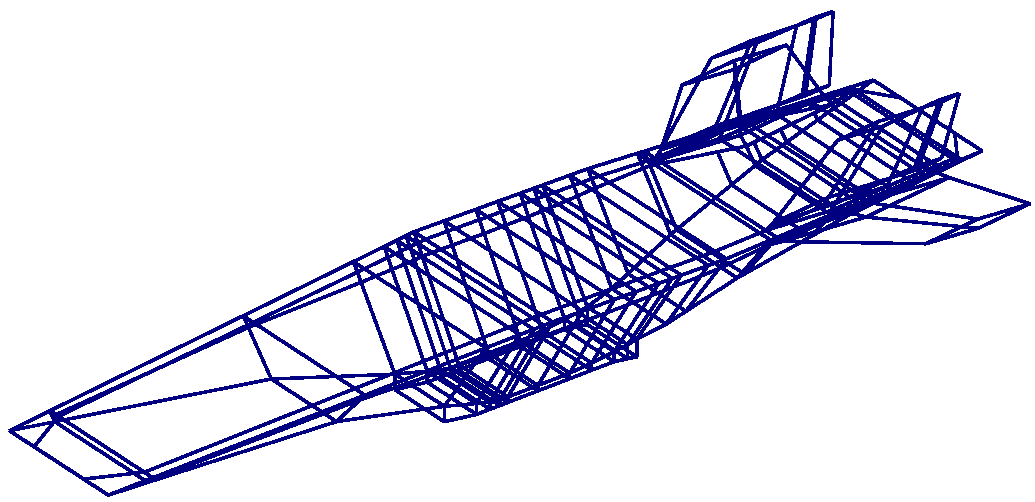
\includegraphics[width=4in]{./pics/frontispiece.pdf}}

% front page style
%\frontpagestyle{1}

% Dedication
%\dedication

% acknowledgments
% set width of acknowledgments as fraction of total \textwidth
%\acknowledgments[6]
%\acknowledgmentswidth{0.8}

% preface
%\preface[2]{ %
%}

% committee
\committee{%
	Professor Jeffrey A. Fessler, Co-Chair \\
	Assistant Research Scientist Jon-Fredrik Nielsen, Co-Chair \\
	Professor Douglas C. Noll \\
	Associate Professor Clayton Scott \\
	Associate Research Scientist Scott Swanson
}%

% chair entered separately for formatting
\cochair{%
	Jeffrey A. Fessler and Jon-Fredrik Nielsen
}%

% hide/show lists of figures, tables, etc.
\showlistoftables
\hidelistofprograms
\showlistofappendices
\hidelistofabbreviations
\hidelistofacronyms

% abbreviations
\begin{comment}
\abbreviations{%
 \acro{CFD}{Computational Fluid Dynamics}
 \acro{MSRSF}{Monotonic, Single-Root Scalar Function}
}%
\end{comment}

% abstract
\abstract{%
	todo
}%
\hideabstractpagenumber

% document
\begin{document}

% chapters
\chapter{Introduction}
\label{c,intro}
% introduction

Magnetic resonance imaging (MRI)
is a non-invasive tool
that has earned widespread clinical adoption
due (among other reasons) 
to its potential for excellent soft tissue contrast,
its absence of ionizing radiation,
and its flexibility to characterize 
a diversity of physical phenomena. 
Despite its numerous advantages,
MRI requires highly specialized hardware,
ongoing liquid-helium cooling
of its superconducting main magnet,
and long scan times.
For these reasons,
MRI is expensive relative
to other medical imaging modalities.
To better focus expenditures,
one broad initiative advocated by the MR community 
is to increase the \emph{value}
of MRI examinations.
One popular (and ambitious) measure of value
is an MRI acquisition's specificity
in distinguishing one disorder
from a collection of candidates.
The field of quantitative MRI (QMRI)
seeks to estimate MR \emph{biomarkers},
or measurable tissue properties
that may be indicative 
of specific disorders of interest.

QMRI has potential
to be more informative than conventional MRI.
Conventional MRI is qualitative:
it produces images comprised of voxels
(\ie, three-dimensional pixels)
that are informative only relative to each other,
not individually.
Conventional MRI voxels are qualitative
because they directly localize the MR signal,
a typically complex function
of not only biomarkers
but also two types of confounds:
\emph{nuisance markers}
that characterize undesired signal sources
and/or MRI system imperfections;
and \emph{acquisition parameters}
that characterize the MRI system's tunable ``knobs''. 
QMRI seeks to remove confound influence
by instead imaging the biomarkers directly.
Each QMR image voxel
is thus a measurement 
of a given biomarker
at a specific location.
QMRI can therefore provide localized biomarker measurements
(\eg, myelin water content)
related to a specific physiological process
(\eg, demyelination)
that can through longitudinal study
be used to monitor the onset and progression of disease
(\eg, multiple sclerosis).

QMRI poses several challenges
beyond those of conventional MRI 
that currently limit its feasibility 
for routine clinical use.
For example,
accurate biomarker quantification 
traditionally requires multiple MR scans
and thus long scan times.
Furthermore,
it has previously been unclear
how to tune acquisition parameters 
of these multiple scans
to ensure that biomarkers can be quantified precisely.
Finally, MR biomarker quantification
is a challenging estimation problem
for which efficient algorithms
have previously been unavailable.
Addressing these challenges is essential
for widespread clinical adoption of QMRI.

\section{Overview}
\label{s,intro,over}

This thesis seeks
to address the above challenges
by developing an automated workflow for QMRI.
We exploit tools
from optimization, statistics, and machine learning
to develop fast algorithms
for quantifying biomarkers
that characterize specific physiological processes. 
We apply this framework
to challenging QMRI problems 
of clinical interest.
Our goal is to introduce fast, automated tools
that will increase the clinical value of QMRI.

Our solutions to two distinct subproblems in QMRI
constitute two stages of our proposed QMRI workflow.
Questions in \emph{acquisition design}
(Chapters~\ref{c,scn-dsgn}, \ref{c,mwf})
ask how to assemble 
fast collections of scans
that yield data 
rich in information 
about physical processes of interest.
Questions in \emph{parameter estimation}
(Chapters~\ref{c,relax}, \ref{c,perk})
ask how to quickly and reliably quantify biomarkers 
associated with these relevant physical processes.
The overall workflow seeks to
first design fast and informative scans 
based on the application,
and to then accurately and precisely estimate 
clinically relevant biomarkers.
 
\section{Organization}
\label{s,intro,org}

The main body of this thesis is organized as follows.
\edit{%
	Within this main body,
	Chapters~\ref{c,scn-dsgn}-\ref{c,mwf}
	organize the key contributions to science
	of this thesis.
}%
\begin{itemize}
\setlength\itemsep{0.5em}
	\item{% 
		Chapter~\ref{c,bkgrd} reviews 
		relevant background material
		on MRI and optimization.
	}%
	\item{% 
		Chapter~\ref{c,relax} discusses methods 
		for QMRI parameter estimation 
		from likelihood models 
		and applies these methods 
		for model-based MR relaxometry,
		a simple and popular application.
		It partially derives content
		from conference papers 
		\cite{nataraj:14:rje,nataraj:14:mbe}.
	}%
	\item{%
		Chapter~\ref{c,scn-dsgn} introduces
		a minimax optimization problem
		to aid robust and application-specific 
		MR scan selection and optimization 
		for precise latent parameter estimation.
		It optimizes several practical acquisitions 
		and uses the likelihood-based estimation techniques 
		introduced in Chapter~\ref{c,relax}
		to assess the utility
		of scan optimization
		through simulations 
		as well as phantom and \invivo experiments.
		It mainly derives content
		from published journal paper
		\cite{nataraj:17:oms}
		that extends conference paper
		\cite{nataraj:15:amm}.
	}%
	\item{% 
		Chapter~\ref{c,perk} introduces
		a fast, general algorithm
		for dictionary-free QMRI parameter estimation
		via regression with kernels (PERK).
		It demonstrates orders-of-magnitude acceleration 
		over likelihood-based estimators
		through simulations
		as well as phantom and \invivo experiments.
		It also characterizes PERK performance
		through bias-covariance analysis 
		and several robustness studies.
		It mainly derives content 
		from accepted journal paper
		\cite{nataraj::dfm} 
		that extends two conference papers
		\cite{nataraj:17:dfm,nataraj:17:slw}.
	}%
	\item{%
		Chapter~\ref{c,mwf} introduces a new method 
		for imaging an MR biomarker of clinical interest. 
		It applies ideas 
		developed in earlier chapters
		to design a new fast QMRI workflow
		that may be specific to healthy myelin,
		whose degradation is associated
		with certain white matter disorders.
		It demonstrates this new method 
		of potentially myelin-specific imaging
		in simulations and \invivo experiments.
		It partially derives content 
		from in-preparation journal paper \cite{nataraj::fmw}
		that extends conference paper \cite{nataraj:17:mwf}.
	}%
	\item{% 
		Chapter~\ref{c,future} suggests 
		several future research directions.
	}%
\end{itemize}

\vspace{0.5em}
{\setlength{\parindent}{0ex}
The appendices contain unpublished, less mature work
and are organized as follows:}
\begin{itemize}
	\setlength\itemsep{0.5em}
	\item{%
		Appendix~\ref{a,cc-multi} proposes an algorithm
		for simultaneously coil-combining 
		a collection of MR coil image datasets
		without prior knowledge 
		of coil sensitivity maps.
		Several chapters in the main body 
		used this algorithm for coil data combination.
	}%
	\item{%
		Appendix~\ref{a,ss-rf} develops 
		from first principles a new model
		for the influence of RF pulses
		on the steady-state (SS) transverse magnetization
		and then proposes two algorithms
		for SS-informed RF pulse design.
	}%
%	\item{%
%		Appendix~\ref{a,dess-diff} presents an analysis
%		of model mismatch due to the presence of diffusion,
%		demonstrates that neglecting diffusive effects
%		during $\Tt$ estimation 
%		can cause significant bias,
%		and suggests acquisition modifications
%		for mitigating this bias.
%	}%
\end{itemize}


\chapter{Background}
\label{c,bkgrd}
% background

This chapter focuses
only on background information 
pertinent to multiple subsequent chapters.
We present further topic-specific information 
at the beginnings 
of corresponding chapters.
Section~\ref{s,bkgrd,mri} places emphasis
on reviewing necessary MR fundamentals,
and Section~\ref{s,bkgrd,opt}
proceeds to a shorter discussion
regarding optimization
as it pertains to QMRI.

\section{Relevant MR Physics}
\label{s,bkgrd,mri}

This section begins
with the fundamental Bloch equations
and derives the signal models
associated with 
two MR pulse sequences
used extensively in this thesis.
Our coverage of MRI
is far from comprehensive, 
and omits fundamental but tangential topics
such as signal localization.
We refer the interested reader
to books such as 
\cite{macovski:83,haacke:99,nishimura:96:pom}.

\subsection{Bloch Equations}
\label{ss,bkgrd,mri,bloch}

The Bloch equations
\cite{bloch:1946:ni-paper}
describe the magnetization dynamics
of \emph{spins}, 
or (loosely) atomic nuclei with nonzero 
angular momentum
and thus nonzero magnetic moment,
\eg $^1$H.
If the dominant source
of magnetic flux 
arises 
(as is typical in MRI)
from a main magnetic field
that is oriented along the $z$-axis,
the equations read
\begin{align}
	\dela{t} \mxy\prt &= i\gam\paren{\mz\prt \bxy\prt - \mxy\prt \bz\prt} -
		\frac{\mxy\prt}{\Tt\pr} ;
		\label{eq:bloch-mxy} \\
	\dela{t} \mz\prt &= \gam\paren{\mx\prt \by\prt - \my\prt \bx\prt} - 
		\frac{\mz\prt - \mzero\pr}{\To\pr}.
		\label{eq:bloch-mz}
\end{align}
Here, 
$\mxy\prt := \mx\prt + i\my\prt \in \complex$
and
$\mz\prt \in \real$
are the transverse and longitudinal components 
of the magnetization vector
at position $\bmr := [x, y, z]\tpose \in \reals{3}$ 
and time $t\geq0$;
$\bxy\prt := \bx\prt + i\by\prt \in \complex$
and 
$\bz\prt \in \real$
are the transverse and longitudinal components 
(in an inertial reference frame)
of the applied magnetic field;
$\To\pr$ and $\Tt\pr$
are spin-lattice and spin-spin relaxation time constants;
$\mzero\pr$ 
is the equilibrium magnetization
and is proportional to the density
of spins per unit volume
as well as the main field strength;
$\gam$
is the gyromagnetic ratio;
and $i := \sqrt{-1}$.
As written,
equations \eqref{eq:bloch-mxy}-\eqref{eq:bloch-mz}
only model dominant temporal dynamics;
later chapters consider second-order effects
such as multiple magnetization compartments
(Chapter~\ref{c,mwf})
and diffusion
(Appendix~\ref{a,dess-diff}).

It is often convenient 
to study Bloch dynamics in a non-inertial reference frame
rotating clockwise about the $z$-axis 
at Larmor frequency 
$\omzero := \gam \Bzero$,
where 
$\Bzero \unit{k}$
is the (nearly uniform) main magnetic field.
In these coordinates,
the apparent transverse magnetic field 
$\bxyp\prt = \bxp\prt + i\byp\prt := \bxy\prt e^{i\omzero t}$
transforms only in phase,
but the apparent longitudinal magnetic field
$\bzp\prt := \bz\prt - \Bzero$
is greatly reduced in magnitude.
The magnetization components transform more simply as
$\mxyp\prt = \mxp\prt + i\myp\prt := \mxy\prt e^{i\omzero t}$
and 
$\mzp\prt := \mz\prt$.
Remarkably, inserting these coordinate transformations 
into \eqref{eq:bloch-mxy}-\eqref{eq:bloch-mz} 
does not change the form
of the dynamical equations:
\begin{align}
	\dela{t} \mxyp\prt &= i\gam\paren{\mzp\prt \bxyp\prt - \mxyp\prt \bzp\prt} -
		\frac{\mxyp\prt}{\Tt\pr} ;
		\label{eq:bloch-mxyp} \\
	\dela{t} \mzp\prt &= \gam\paren{\mxp\prt \byp\prt - \myp\prt \bxp\prt} - 
		\frac{\mzp\prt - \mzero\pr}{\To\pr}.
		\label{eq:bloch-mzp}
\end{align}
It thus suffices to consider 
how perturbations $\bmbp\prt$
to main field $\Bzero \unit{k}$ 
influence rotating-frame magnetization $\bmmp\prt$
via Eqs.~\eqref{eq:bloch-mxyp}-\eqref{eq:bloch-mzp}.
The inertial-frame magnetization $\bmm\prt$ 
is then easily constructed via
$\mxy\prt = \mxyp\prt e^{-i\omzero t}$ 
and $\mz\prt = \mzp\prt$.

It is challenging
to explicitly solve Eqs.~\eqref{eq:bloch-mxyp}-\eqref{eq:bloch-mzp}
for arbitrary field perturbations $\bmbp\prt$. 
We discuss relevant special cases 
in the following.

\subsubsection{Non-Selective Excitation}
\label{sss,bkgrd,mri,bloch,ex}

Here,
we derive solutions 
to Eqs.~\eqref{eq:bloch-mxyp}-\eqref{eq:bloch-mzp}
in the case of short, spatially non-selective excitations.
We take the following common assumptions:
\begin{itemize}
	\item 
		We assume negligible spatial variation
		in the longitudinal magnetic field, 
		so $\bzp\prt \approx 0$. 
		This lack of spatial variation is reason
		for non-selective excitation.
	\item 
		We assume the transverse field
		separates in position and time;
		oscillates at the Larmor frequency
		(commonly in the radiofrequency (RF) range);
		and aligns at initial time $t \gets t_0$ 
		with the $x$-axis.
		Together,
		these assumptions restrict
		the so-called RF excitation to take form
		$\bxyp\prt \approx \stx\pr \bonexp\pt \unit{i} + 0\unit{j}$,
		where $\stx\pr \in \real$ is the RF transmit coil spatial variation
		and $\bonexp\pt \in \real$ is the RF excitation envelope.
	\item
		We assume that 
		the duration $\TP$
		of RF excitation
		(often $\TP\sim$1ms)
		is much shorter than relaxation time constants
		(typically $\To\sim$1000ms and $\Tt\sim$50ms
		in brain tissue)
		and thus neglect relaxation effects
		during excitation.
\end{itemize}
Under these assumptions, 
Eqs.~\eqref{eq:bloch-mxyp}-\eqref{eq:bloch-mzp}
reduce to the linear system
\begin{align}
	\dela{t}
	\begin{bmatrix}
		\mxp\prt \\
		\myp\prt \\
		\mzp\prt
	\end{bmatrix}
	=
	\begin{bmatrix}
		0 & 0 & 0 \\
		0 & 0 & \gam \stx\pr \bonexp\pt \\
		0 & -\gam \stx\pr \bonexp\pt & 0
	\end{bmatrix}
	\begin{bmatrix}
		\mxp\prt \\
		\myp\prt \\
		\mzp\prt
	\end{bmatrix}.
	\label{eq:bloch-rot}
\end{align}
Eq.~\eqref{eq:bloch-rot} admits the simple solution
(for $t\geq t_0$)
\begin{align}
	\begin{bmatrix}
		\mxp\prt \\
		\myp\prt \\
		\mzp\prt
	\end{bmatrix}
	= 
	\begin{bmatrix}
		1 & 0 & 0 \\
		0 & \cosa{\fliprt} & \sina{\fliprt} \\
		0 & -\sina{\fliprt} & \cosa{\fliprt} 
	\end{bmatrix}
	\begin{bmatrix}
		\mxp\prtz \\
		\myp\prtz \\
		\mzp\prtz
	\end{bmatrix},
	\label{eq:rot-sol}
\end{align}
where 
$\bmmp\prtz := \brac{\mxp\prtz,\myp\prtz,\mzp\prtz}\tpose$ 
is the initial magnetization and
\begin{align}
	\fliprt := \gam \stx\pr \int_{t_0}^t \bonexp\paren{\tau} \der{\tau} 
	\label{eq:flip-def}
\end{align}
is the nutation (or ``flip'') angle at time $t$.
Eq.~\eqref{eq:rot-sol} reveals 
that on-resonance RF excitation
causes the magnetization vector
to rotate clockwise
about an axis parallel to
the direction of excitation.
The nutation angle
accumulated over an RF pulse 
of duration $\TP$
is often decomposed as
$\flip\prtzt{t_0+\TP} =: \flipnom \stx\pr$,
where $\flipnom$
is a prescribed nominal flip angle.

For deriving signal models
in later sections,
it is convenient and intuitive
to define matrix operators
that summarize relevant dynamics.
Here, we rewrite Eq.~\eqref{eq:rot-sol} as 
\begin{align}
	\bmmp\prt = \bmRxp{\fliprt} \bmmp\prtz,
	\label{eq:mtx-ex}
\end{align}
where $\bmRxp{\fliprt}$ denotes a clockwise rotation
of angle $\fliprt$ 
about the $x'$-axis.

\subsubsection{Free Precession and Relaxation}
\label{sss,bkgrd,mri,bloch,pr}

Next,
we derive solutions
to the rotating-frame Bloch equations
when no RF excitation is present,
\ie $\bxyp\prt \approx 0$.
In this case,
Eqs.~\eqref{eq:bloch-mxyp}-\eqref{eq:bloch-mzp} decouple,
yielding separate dynamical equations
for the transverse and longitudinal magnetization components:
\begin{align}
	\dela{t} \mxyp\prt &= -i\gam \mxyp\prt \bzp\prt - \frac{\mxyp\prt}{\Tt\pr} ;
		\label{eq:bloch-free-mxyp} \\
	\dela{t} \mzp\prt &= -\frac{\mzp\prt - \mzero\pr}{\To\pr}.
		\label{eq:bloch-free-mzp}
\end{align}
Eqs.~\eqref{eq:bloch-free-mxyp}-\eqref{eq:bloch-free-mzp}
admit simple solutions
with no further assumptions: 
\begin{align}
	\mxyp\prt &= \mxyp\prtz e^{-(t-t_0)/\Tt\pr} e^{-i \phprt}; 
		\label{eq:mxy-fp} \\
	\mzp\prt &= \mzp\prtz e^{-(t-t_0)/\To\pr} + \mzero\pr \paren{1-e^{-(t-t_0)/\To\pr}},
		\label{eq:mz-fp}
\end{align}
where $\mxyp\prtz$ and $\mzp\prtz$ 
are the initial magnetization components and
\begin{align}
	\phprt := \gam \int_{t_0}^t \bzp\paren{\bmr,\tau} \der{\tau}
	\label{eq:ph-def}
\end{align}
denotes the phase accumulation
due to main field inhomogeneity
(often called off-resonance effects).
Eq.~\eqref{eq:mxy-fp} reveals that without RF excitations,
the transverse magnetization $\mxyp\prt$
relaxes to zero exponentially fast 
with time constant $\Tt\pr$,
while accruing phase due to off-resonance effects.
Eq.~\eqref{eq:mz-fp} similarly reveals
that without RF excitations,
longitudinal magnetization $\mzp\prt$
recovers to $\mzero\pr$ exponentially fast 
with time constant $\To\pr$.

As in Section~\ref{sss,bkgrd,mri,bloch,pr},
we rewrite Eqs.~\eqref{eq:mxy-fp}-\eqref{eq:mz-fp}
for $t\geq t_0$
using matrix operators:
\begin{align}
	\bmmp\prt = \bmRzp{\phprt} \bmE\prtzt{t} \bmmp\prtz 
		+ \bmmzero\prtzt{t} 
		\label{eq:mtx-pr}
\end{align}
where
$\bmmzero\prtzt{t} := \mzero\pr \paren{1-e^{-(t-t_0)/\To\pr}} \unit{k}$; 
\begin{align}
	\bmRzp{\phprt} :=
	\begin{bmatrix}
		\cosa{\phprt} & \sina{\phprt} & 0 \\
		-\sina{\phprt} & \cosa{\phprt} & 0 \\
		0 & 0 & 1
	\end{bmatrix}
	\label{eq:op-rotz}
\end{align}
denotes a clockwise rotation of angle $\phprt$ about the $z'$-axis; 
and
\begin{align}
	\bmE{\prtzt{t}} := 
	\begin{bmatrix}
		e^{-(t-t_0)/\Tt\pr} & 0 & 0 \\
		0 & e^{-(t-t_0)/\Tt\pr} & 0 \\
		0 & 0 & e^{-(t-t_0)/\To\pr} 
	\end{bmatrix}
	\label{eq:op-relax}
\end{align}
is an exponential relaxation operator.
Section~\ref{ss,bkgrd,mri,ss}
(and later chapters) 
use matrix dynamical representations
\eqref{eq:mtx-ex} and \eqref{eq:mtx-pr}
to succinctly describe pulse sequence
signal models.

\subsection{Steady-State Sequences}
\label{ss,bkgrd,mri,ss}

MRI experiments
typically involve 
repeated cycles of (pulsed) RF excitation;
signal localization (not discussed here);
and transverse $\Tt$ relaxation and free precession, 
alongside (relatively slow) longitudinal $\To$ recovery.
We can build models 
of the received MR signal
by considering the magnetization dynamics
induced by specific pulse sequences.

Classical pulse sequences
use relatively long cycle repetition times $\TR$
to ensure near-complete $\To$ recovery
of the magnetization vector
back to equilibrium state $\mzero\pr \unit{k}$
prior to the start of each RF cycle.
For such long-$\TR$ sequences,
it suffices 
to approximate the magnetization
as fully recovered 
(\ie, $\bmmp\paren{\bmr,t_0 + \rep\TR} \approx \mzero\pr \unit{k}, 
\forall \rep\in\set{0,1,2,\dots}$)
just prior to each RF excitation.
This approximation
yields a sequence of initial conditions
and allows computation of the magnetization
at corresponding times of data acquisition
via direct application of Bloch dynamics
\eqref{eq:mtx-ex} and \eqref{eq:mtx-pr}.
Resulting signal models
are typically simple expressions
of relaxation parameters $\To\pr$ and $\Tt\pr$;
however, model accuracy often depends strongly
on the long-$\TR$ assumption,
which requires long acquisitions.

Steady-state (SS) sequences
\cite{hinshaw:76:ifb}
utilize short $\TR$,
and can thus achieve much faster scan times.
Due to short repetition times,
SS sequences achieve only partial $\To$ recovery
in between RF excitations;
thus, their magnetization responses
do not obey the simple classical initial conditions
(for the second RF cycle onwards).
Although their transient magnetization dynamics
can be complicated,
SS sequences produce
(under certain assumptions \cite{scheffler:99:apd})
long-time magnetization responses
that eventually
\footnote{The progression to steady state takes 
	on the order of 
	$5\Tt/\TR$ RF cycles \cite{scheffler:99:apd},
	typically a small but not insignificant period 
	during which data acquisition is often foregone. 
	This transition can
	(in some cases) be accelerated 
	by prepending SS sequences
	with tailored ``magnetization-catalyzing'' modules
	\cite{hargreaves:01:car}.
}
achieve a
steady-state condition:
\begin{align}
	\lim_{t_0 \to \infty} \bmmp\paren{\bmr,t_0+\rep\TR} = \bmmp\paren{\bmr,t_0},
	\label{eq:ss-cond}
\end{align}
where repetition count 
$\rep \in \set{1,2,\dots}$
for fixed RF excitations
and off-resonance induced phase increments
(as is assumed in the following).
Subsections~\ref{sss,bkgrd,mri,ss,spgr}
and \ref{sss,bkgrd,mri,ss,dess}
use SS condition \eqref{eq:ss-cond}
and Bloch equation matrix operators
introduced in
\eqref{eq:mtx-ex} and \eqref{eq:mtx-pr}
to derive long-time signal models
for Spoiled Gradient-Recalled Echo (SPGR)
and Dual-Echo Steady-State (DESS),
two SS pulse sequences
useful for quantitative MRI.

\subsubsection{Spoiled Gradient-Recalled Echo (SPGR) Sequence}
\label{sss,bkgrd,mri,ss,spgr}

SPGR \cite{zur:91:sot}
is a fast pulse sequence
that repeats cycles of 
fixed RF excitation
(such that $\bonexp\paren{t+\rep\TR} = \bonexp\pt,
\forall t\in\brac{t_0,t_0+\TP}, r\in\set{1,2,\dots}$);
data acquisition;
relaxation and recovery;
and residual transverse magnetization ``spoiling''
(discussed later).
Here we develop
a simple and popular steady-state SPGR signal model.

Let $\bmmp\prtz$ denote the magnetization
at an initial time $t_0$ 
selected well into the steady-state
and just prior to excitation.
The SPGR sequence first applies
an RF excitation, 
which rotates the initial magnetization
as per \eqref{eq:mtx-ex}:
\begin{align}
	\bmmp\paren{\bmr,t_0+\TP} = \bmRxp{\flip\prtzt{t_0+\TP}} \bmmp\prtz.
	\label{eq:spgr-ex}
\end{align}
The excited magnetization 
then precesses and relaxes
as per \eqref{eq:mtx-pr}
until data acquisition,
defined to occur at
``echo time'' $\TE \in \brac{\TP,\TR}$
after the (midpoint of) RF excitation:
\begin{align}
	\bmmp\paren{\bmr,t_0+\frac{\TP}{2}+\TE} &=
	\bmRzp{\php\paren{\bmr,\frac{\TP}{2}+\TE;\TP}} 
	\bmE\paren{\bmr,\frac{\TP}{2}+\TE;\TP} \bmmp\paren{\bmr,t_0+\TP} \nonumber \\
	&+ \bmmzero\paren{\bmr,\frac{\TP}{2}+\TE;\TP}.
	\label{eq:spgr-daq}
\end{align}
Following signal reception,
the remaining transverse magnetization 
is spoiled 
\footnote{Transverse signal spoiling 
is often (nearly) achieved in practice
using strong induced field inhomogeneities 
(which cause rapid transverse signal dephasing)
in tandem with RF excitations
that additionally impart nonlinear
(often quadratically increasing)
transverse magnetization phase
\cite{zur:91:sot}.
Though the nonlinear RF phase
used in so-called ``RF-spoiling'' 
prevents any one spin
from reaching a true steady-state,
the signal integrated
over a typically-sized voxel
achieves SS-like behavior
\cite{denolin:05:nii}.
}
while the longitudinal component
is unaffected. 
We model an ideal spoiling operation as
\begin{align}
	\bmS \bmmp\paren{\bmr,\frac{\TP}{2}+\TE}, \where \qquad
	\bmS := 
	\begin{bmatrix}
		0 & 0 & 0 \\
		0 & 0 & 0 \\
		0 & 0 & 1
	\end{bmatrix}.
	\label{eq:spgr-spoil}
\end{align}
After spoiling, 
the longitudinal magnetization 
(partially) recovers
until $t \gets t_0+\TR$:
\begin{align}
	\bmmp\paren{\bmr,t_0+\TR} &= 
	\bmRzp{\php\paren{\bmr,\TR;\frac{\TP}{2}+\TE}} 
	\bmE\paren{\bmr,\TR;\frac{\TP}{2}+\TE} \bmS 
	\bmmp\paren{\bmr,t_0+\frac{\TP}{2}+\TE} \nonumber \\
	&+ \bmmzero\paren{\bmr,\TR;\frac{\TP}{2}+\TE}.
	\label{eq:spgr-pr}
\end{align}
In steady-state, 
one cycle of excitation, acquisition, spoiling, and recovery 
returns the magnetization back to its initial state.
We enforce this through the steady-state condition
\begin{align}
	\bmmp\paren{\bmr,t_0+\TP} = \bmRxp{\flip\prtzt{t_0+\TP}} \bmmp\paren{\bmr,t_0+\TR}
	\label{eq:spgr-ss}
\end{align}
which yields an algebraic
system of equations.
When it exists,
the solution is
\begin{align}
	\bmmp\paren{\bmr,t_0+\TP} = 
	\frac{1}{1-e^{-\paren{\TR-\TP}/\To\pr}\cosa{\alpha\pr}}
	\begin{bmatrix}
		0 \\
		\mzero\pr \sina{\flip\pr} \paren{1-e^{-\paren{\TR-\TP}/\To\pr}}\\
		\mzero\pr \cosa{\flip\pr} \paren{1-e^{-\paren{\TR-\TP}/\To\pr}}
	\end{bmatrix},
	\label{eq:spgr-bmmp-t0}
\end{align}
where $\flip\pr := \flip\prtzt{t_0+\TP}$ 
is a slight abuse of notation.
Remarkably, 
the SPGR steady-state magnetization
immediately after excitation
is approximately independent
of both off-resonance effects
and $\Tt\pr$.
Researchers more often cite the expression
\begin{align}
	\mxyp\paren{\bmr,t_0+\TP}
	&= \mxp\paren{\bmr,t_0+\TP} + i\myp\paren{\bmr,t_0+\TP} \nonumber \\
	&= \frac{i\mzero\pr \sina{\flip\pr} \paren{1-e^{-\TR/\To\pr}}}
	{1-e^{-\TR/\To\pr}\cosa{\alpha\pr}}
	\label{eq:spgr-mxyp-t0}
\end{align}
for the complex transverse magnetization
as it modifies \eqref{eq:spgr-bmmp-t0}
to include a simple first-order correction
for unaccounted $\To$ recovery during the RF pulse.
Substituting \eqref{eq:spgr-mxyp-t0} 
into \eqref{eq:spgr-daq} 
yields an expression 
for the transverse magnetization
at the echo time:
\begin{align}
	\mxyp\paren{\bmr,t_0+\frac{\TP}{2}+\TE} 
	&=
	\mxyp\paren{\bmr,t_0+\TP} 
	e^{-(\TE-\TP/2)/\Tt\pr} 
	e^{-i\php\paren{\bmr,t_0+\frac{\TP}{2}+\TE;t_0+\TP}} \nonumber \\
	&\approx
	\mxyp\paren{\bmr,t_0+\TP} 
	e^{-\TE/\Tt\pr} 
	e^{-i\php\paren{\bmr,t_0+\frac{\TP}{2}+\TE;t_0+\frac{\TP}{2}}},
	\label{eq:spgr-mxyp-te}
\end{align}
where the approximation
again keeps in line 
with literature expressions.

The received signal
is approximately proportional 
to the integrated transverse magnetization
over a volume $\setV$.
To derive expressions,
we take a few more usual assumptions:
\begin{itemize}
	\item We assume that
	the signal is localized
	to a scale over which
	there is off-resonance phase variation,
	but minimal variation
	of $\mzero\pr$, $\To\pr$, $\Tt\pr$, and $\flip\pr$.
	This assumption is reasonable
	\footnote{Model mismatch due
		to within-voxel spatial variation 
		of relaxation parameters
		can be significant,
		especially for large voxels.
		Chapter~\ref{c,mwf} studies 
		so-called partial volume effects
		and uses them for QMRI.
	} 
	when describing the signal 
	arising from a typical voxel.
	\item We assume that
	(free-precession) off-resonance phase 
	grows linearly with time,
	\ie $\php\paren{\bmr,t_0+\frac{\TP}{2}+\TE;t_0+\frac{\TP}{2}} \approx \omp\pr \TE$.
	We further assume
	that off-resonance frequency $\omp\pr$
	is distributed over the localized voxel
	as $\dist{\omp} \gets \operatorname{Cauchy}\paren{\ompmed,\Rtp}$,
	where $\ompmed\pr$ is the median off-resonance frequency
	and $\Rtp\pr$ is the broadening bandwidth.
\end{itemize}
With these additional assumptions,
the received steady-state SPGR (noiseless) signal model
for a typically sized voxel
centered at position $\bmr$ is (to within constants):
\begin{align}
	\spgr\paren{\bmr,t_0+\frac{\TP}{2}+\TE} 
	&\propto \int_{\setV\pr} \mxyp\paren{\bmr,t_0+\frac{\TP}{2}+\TE} \dercubed{\bmr} 
		\label{eq:spgr-int} \\
	&\approx \mxy\paren{\bmr,t_0+\TP} e^{-\TE/\Tt\pr} \int_\real e^{-i\omp \TE} 
		\dist{\omp}\paren{\omp} \der{\omp} \nonumber \\
	&= \mxy\paren{\bmr,t_0+\TP} e^{-\TE/\Tt\pr} e^{-\Rtp\pr\TE - i\ompmed\pr\TE} \nonumber \\
	&= \frac{i\mzero\pr \sina{\flip\pr} \paren{1-e^{-\TR/\To\pr}}}
	{1-e^{-\TR/\To\pr}\cosa{\alpha\pr}} e^{-\TE/\Tts\pr} e^{-i\ompmed\pr \TE},
		\label{eq:spgr-model}
\end{align}
where $\Tts\pr := \inv{\frac{1}{\Tt} + \Rtp}$
is a modified spin-spin relaxation time
that accounts for additional transverse magnetization decay
due to off-resonance effects.

\subsubsection{Dual-Echo Steady-State (DESS) Sequence}
\label{sss,bkgrd,mri,ss,dess}

DESS \cite{redpath:88:fan,bruder:88:ans}
is a fast pulse sequence 
that interlaces fixed, constant-phase RF excitations
with fixed dephasing ``gradients''
(\ie, induced main field inhomogeneities 
that vary nearly linearly with space)
to produce two distinct signals
per RF excitation.
Here we develop simple 
steady-state DESS signal models.

As in Subsection~\ref{sss,bkgrd,mri,ss,spgr},
let $\bmmp\prtz$ denote the magnetization
at an initial time $t_0$ 
selected well into the steady-state
and just prior to excitation.
The DESS sequence first applies
a fixed RF rotation
$\flip\pr := \flip\paren{\bmr,t_0+\rep\TR+\TP;t_0+\rep\TR},
\forall r \in \set{0,1,2,\dots}$:
\begin{align}
	\bmmp\paren{\bmr,t_0+\TP} = \bmRxp{\flip{\pr}} \bmmp\prtz.
	\label{eq:dess-ex}
\end{align}
The excited transverse magnetization
contributes to a first acquired signal;
dephases (but does not spoil completely) 
due to gradient dephasing
\footnote{It is worth distinguishing 
gradient dephasing
(commonly 
but somewhat misleadingly 
referred to as gradient spoiling)
from RF spoiling.
Gradient dephasing
(used in DESS)
primarily affects magnetization phase
and is modeled simply as precession.
RF spoiling
(used in SPGR)
combines gradient dephasing 
with nonlinear RF phase cycling
and suppresses magnetization magnitude 
in steady-state.
}
and contributes again to a second 
(smaller, but nonzero) acquired signal.
Since (with proper selection) 
dephasing gradients mainly contribute 
to off-resonance phase accrual,
the net effect
after data acquisition
and gradient spoiling
is well described 
simply by precession and relaxation:
\begin{align}
	\bmmp\paren{\bmr,t_0+\TR} &= 
	\bmRzp{\php\paren{\bmr}} \bmE\paren{\bmr,\TR;\TP} \bmmp\paren{\bmr,t_0+\TP} +
	\bmmzero\paren{\bmr,\TR;\TP},
	\label{eq:dess-pr}
\end{align}
where the abbreviation
$\php\pr := \php\paren{\bmr,t_0+\paren{\rep+1}\TR;t_0+\rep\TR+\TP},
\forall \rep \in \set{0,1,2,\dots}$
implies fixed phase accrual 
(due to gradient dephasing, 
field inhomogeneity, 
and other unaccounted effects)
over each repetition cycle.

In steady-state,
one cycle of excitation,
first acquisition, 
gradient spoiling,
second acquisition,
and (partial) recovery
returns the magnetization
back to its initial state.
We enforce this
through the steady-state condition
\begin{align}
	\bmmp\prtz = \bmmp\paren{\bmr,t_0+\TR}
	\label{eq:dess-ss}
\end{align}	
which yields an algebraic system of equations.
When it exists, 
the solution gives 
the steady-state magnetization
just prior to RF excitation:
\begin{align}
	\bmmp\prtz =
	\begin{bmatrix}
		\EtRP \sin{\flip\pr} \sin{\php\pr} \\
		-\EtRP \sin{\flip\pr} \paren{\EtRP-\cos{\php\pr}} \\
		1-\EtRP\cos{\php\pr} + \EtRP \cos{\flip\pr} \paren{\EtRP-\cos{\php\pr}}
	\end{bmatrix}
	q\paren{\bmr,\TFP},
	\label{eq:dess-bmmp-t0}
\end{align}
where 
$\TFP := \TR-\TP$ 
is the free precession interval;
$\Eo\paren{\bmr,t} := e^{-t/\To\pr}$ and 
$\Et\paren{\bmr,t} := e^{-t/\Tt\pr}$
are relaxation operators;
and 
$q\paren{\bmr,t} := $
$$
\frac{\mzero\pr \paren{1-\Eo\prt}
}{\paren{1-\Eo\prt\cos\flip\pr} \paren{1-\Et\prt\cos\php\pr} -
\Et\prt \paren{\Eo\prt - \cos\flip\pr} \paren{\Et\prt - \cos\php\pr}}.
$$
Substituting \eqref{eq:dess-bmmp-t0} 
into \eqref{eq:dess-ex}
produces a similar expression 
for the steady-state magnetization
immediately following RF excitation:
\begin{align}
	\bmmp\paren{\bmr,t_0+\TP} =
	\begin{bmatrix}
		\EtRP \sin{\flip\pr} \sin{\php\pr} \\
		\sin{\flip\pr} \paren{1 - \EtRP \cos{\php\pr}} \\
		\cos{\flip\pr} \paren{1 - \EtRP \cos{\php\pr}} + \EtRP \paren{\EtRP - \cos{\php\pr}}
	\end{bmatrix}
	q\paren{\bmr,\TFP}.
	\label{eq:dess-bmmp-tp}
\end{align}
The transverse magnetizations
before and after RF excitation are then
\begin{align}
	\mxyp\prtz &= 
		-i\sin{\flip\pr} \EtR \paren{\EtR-e^{-i\php\pr}} q\paren{\bmr,\TR}
		\label{eq:dess-mxyp-t0}; \\
	\mxyp\paren{\bmr,t_0+\TP} &=
		+i\sin{\flip\pr} \paren{1-\EtR e^{i\php\pr}} q\paren{\bmr,\TR},
		\label{eq:dess-mxyp-tp}
\end{align}
where \eqref{eq:dess-mxyp-t0}-\eqref{eq:dess-mxyp-tp}
include simple first-order corrections
for yet-unaccounted relaxation and recovery
during excitation.
Frequently, 
the DESS signals are acquired 
at symmetric echo times $\TE$
before and after the center of each RF pulse.
Substituting \eqref{eq:dess-mxyp-tp} 
into \eqref{eq:bloch-free-mxyp}
gives the magnetization
at the data acquisition time
after RF excitation:
\begin{align}
	\mxyp\paren{\bmr,t_0+\frac{\TP}{2}+\TE} 
		&= \mxyp\paren{\bmr,t_0+\TP} e^{-\paren{\TE-\TP/2}/\Tt\pr} 
			e^{-i\php\paren{\bmr,t_0+\frac{\TP}{2}+\TE;t_0+\TP}} \nonumber \\
		&\approx \mxyp\paren{\bmr,t_0+\TP} e^{-\TE/\Tt\pr} 
			e^{-i\php\paren{\bmr,t_0+\frac{\TP}{2}+\TE;t_0+\frac{\TP}{2}}}
			\label{eq:dess-mxyp-te1-ph} \\
		&\approx \mxyp\paren{\bmr,t_0+\TP} e^{-\TE/\Tt\pr} e^{-i\omp\pr\TE},	
			\label{eq:dess-mxyp-te1}
\end{align}
where in \eqref{eq:dess-mxyp-te1-ph}
we again approximately correct
for relaxation during excitation
and in \eqref{eq:dess-mxyp-te1}
we assume linear off-resonance phase accrual 
during free precession.
To compute the magnetization
at the acquisition time 
before excitation,
we consider the free precession and relaxation
that occurs between 
\footnote{Observe that we do not attempt
to express the magnetization 
prior to (the next) RF excitation
by simply operating on the magnetization after (the current) RF excitation
with further precession and relaxation.
The reason is due to the intermediate dephasing gradient,
which causes phase accrual
in excess of off-resonance effects
and thus forbids an approximation akin to \eqref{eq:dess-mxyp-te1}.
}
signal reception and excitation:
\begin{align}
	\mxyp\paren{\bmr,t_0} =
		\mxyp\paren{\bmr,t_0-\paren{\TE-\frac{\TP}{2}}} e^{-\paren{\TE-\TP/2}/\Tt\pr} e^{-i\php\paren{\bmr,t_0;t_0-\paren{\TE-\frac{\TP}{2}}}}.
		\label{eq:dess-mxyp-pr-te2}
\end{align}
Rearranging \eqref{eq:dess-mxyp-pr-te2} 
and applying approximations
similar to those of 
\eqref{eq:dess-mxyp-te1-ph}-\eqref{eq:dess-mxyp-te1},
\begin{align}
	\mxyp\paren{\bmr,t_0+\frac{\TP}{2}-\TE} 
		&= \mxyp\paren{\bmr,t_0} e^{+\paren{\TE-\TP/2}/\Tt\pr} 
			e^{+i\php\paren{\bmr,t_0;t_0-\paren{\TE-\frac{\TP}{2}}}} \nonumber \\
		&\approx \mxyp\paren{\bmr,t_0} e^{+\TE/\Tt\pr} 
			e^{+i\php\paren{\bmr,t_0+\frac{\TP}{2};t_0+\frac{\TP}{2}-\TE}}
			\label{eq:dess-mxyp-te2-ph} \\
		&\approx \mxyp\paren{\bmr,t_0} e^{+\TE/\Tt\pr} e^{+i\omp\pr\TE}.	
			\label{eq:dess-mxyp-te2}
\end{align}

The received signal is approximately proportional
to the integrated transverse magnetization 
over a volume $\setV$.
To derive expressions,
we retake assumptions used
in Subsection~\ref{sss,bkgrd,mri,ss,spgr}
and append an additional assumption
on the full-repetition phase accrual $\php\pr$:
\begin{itemize}
	\item We assume that
		the signal is localized
		to a scale over which
		there is off-resonance phase variation,
		but minimal variation
		of $\mzero\pr$, $\To\pr$, $\Tt\pr$, and $\flip\pr$.
		This assumption is reasonable
		\footnote{Model mismatch due
			to within-voxel spatial variation 
			of relaxation parameters
			can be significant,
			especially for large voxels.
			Chapter~\ref{c,mwf} studies 
			so-called partial volume effects
			and uses them for QMRI.
		} 
		when describing the signal 
		arising from a typical voxel.
	\item We assume that
		free precession off resonance frequency $\omp\pr$
		is distributed over the localized voxel
		as $\dist{\omp} \gets \operatorname{Cauchy}\paren{\ompmed,\Rtp}$,
		where $\ompmed\pr$ is the median off-resonance frequency
		and $\Rtp\pr$ is the broadening bandwidth.
	\item We assume that 
		the dephasing gradient imparts 
		an integral number $\cyc$ of across-voxel phase cycles
		\footnote{In theory,
			it suffices to design dephasing gradients
			to impart as few as one complete cycle
			of net phase variation across a voxel.
			In practice,
			field inhomogeneities will induce
			spurious through-voxel field gradients 
			that modify the effective dephasing gradient moment
			and thereby create partial phase cycles
			that distort the nominally uniform phase distribution.
			To reduce model mismatch 
			due to such ``partial spoiling'' effects,
			dephasing gradients are usually designed
			to nominally impart multiple complete cycles
			of across-voxel phase variation.
			However, 
			larger dephasing gradients
			cause greater DESS model mismatch
			due to diffusive signal loss.
			Appendix~\ref{a,dess-diff} 
			studies diffusion in DESS
			and discusses regimes of dephasing gradient moments
			which balance partial-spoiling versus diffusive
			sources of model mismatch.
		}
		such that full-repetition phase accrual $\php\pr$ 
		is distributed essentially uniformly
		as $\dist{\php} \gets \operatorname{uniform}\paren{0,2\pi\cyc},
		\cyc\in\set{1,2,3,\dots}$.  
\end{itemize}
With these assumptions, 
the received steady-state DESS (noiseless) signal models
for a typically sized voxel centered at position $\bmr$ are
(to within constants):
\begin{align}
	\dess\paren{\bmr,t_0+\frac{\TP}{2}+\TE} 
		&\propto \int_{\setV\paren{\bmr}} 
			\mxyp\paren{\bmr,t_0+\frac{\TP}{2}+\TE} \dercubed{\bmr}
			\label{eq:dess-def-int} \\
		&\approx \int_\real \int_\real \mxyp\paren{\bmr,t_0+\frac{\TP}{2}+\TE} 
			\dist{\php}\paren{\php} \dist{\omp}\paren{\omp} \der{\php} \der{\omp}
			\nonumber \\
		&\approx e^{-\TE/\Tt\pr}
			\int_\real \mxyp\paren{\bmr,t_0+\TP} \dist{\php}\paren{\php} \der{\php} 
			\int_\real e^{-i\omp\TE} \dist{\omp}\paren{\omp} \der{\omp}
			\nonumber \\
		&= +i\mzero\pr \Et\paren{\bmr,\TE} e^{-\paren{\Rtp\pr-i\ompmed\pr}\TE}
			\tan\frac{\alpha\pr}{2} 
			\brac{1 - \frac{\eta\paren{\bmr,\TR}}{\xi\paren{\bmr,\TR}}};
			\label{eq:dess-def-model} \\
	\dess\paren{\bmr,t_0+\frac{\TP}{2}-\TE}
		&\propto \int_{\setV\paren{\bmr}}
			\mxyp\paren{\bmr,t_0+\frac{\TP}{2}-\TE} \dercubed{\bmr}
			\label{eq:dess-ref-int} \\
		&\approx \int_\real \int_\real \mxyp\paren{\bmr,t_0+\frac{\TP}{2}-\TE} 
			\dist{\php}\paren{\php} \dist{\omp}\paren{\omp} \der{\php} \der{\omp}
			\nonumber \\
		&\approx e^{+\TE/\Tt\pr}
			\int_\real \mxyp\paren{\bmr,t_0} \dist{\php}\paren{\php} \der{\php} 
			\int_\real e^{+i\omp\TE} \dist{\omp}\paren{\omp} \der{\omp} 
			\nonumber \\
		&= -i\mzero\pr \Et^{-1}\paren{\bmr,\TE} e^{-\paren{\Rtp\pr+i\ompmed\pr}\TE}
			\tan\frac{\alpha\pr}{2}
			\brac{1 - \eta\paren{\bmr,\TR}},
			\label{eq:dess-ref-model}
\end{align}	
where \eqref{eq:dess-def-model} and \eqref{eq:dess-ref-model}
introduce intermediate variables
\begin{align}
	\eta\prt &:=
		\sqrt{\frac{1-\Et^2\prt}{1-\Et^2\prt/\xi^2\prt}};
		\nonumber \\
	\xi\prt &:=
		\frac{1-\Eo\prt \cos{\flip\pr}}{\Eo\prt - \cos{\flip\pr}}.
		\nonumber
\end{align}
In steady-state, 
the DESS signal is typically greatest 
immediately following excitation 
and defocuses with rate $\frac{1}{\Tt}+\Rtp$
until what we hereafter denote
the \emph{defocusing} echo time.
After a low-signal period between RF pulses,
the DESS signal then refocuses
with rate $\frac{1}{\Tt}-\Rtp$
from what we hereafter denote
the \emph{refocusing} echo time
until just prior the next excitation.
Fortuitously,
the defocusing \eqref{eq:dess-def-model}
and refocusing \eqref{eq:dess-ref-model}
DESS signal models
have significantly different dependence 
on relaxation parameters (especially $\Tt$)
and thus together are quite useful
for relaxation parameter estimation.

\section{Optimization in QMRI}
\label{s,bkgrd,opt}

This section overviews 
how optimization methods are leveraged 
in a substantial portion of this thesis 
to solve practical QMRI problems.
For such problems,
the central idea is to construct
a suitable scalar cost function $\cost$
of some design variables $\bmx$,
whose output $\costa{\bmx} \in \real$ 
is designed to provide a measure
of the undesirability of $\bmx$.
We then employ 
tailored optimization algorithms
to find an $\bmx$
that minimizes $\cost$
over a set $\setX$,
written as
\begin{align}
	\bmx^* \in \set{\argmin{\bmx\in\setX} \costa{\bmx}}.
	\label{eq:opt-global}
\end{align}
In either optimization-based 
parameter estimation (Chapter~\ref{c,relax})
or acquisition design (Chapter~\ref{c,scn-dsgn}),
we have reason to design $\cost$
to depend on corresponding design variables $\bmx$ 
through MR signal models.
Because these models are often 
(strongly) nonlinear functions
of design variables,
corresponding cost functions
are usually non-convex in $\bmx$
(though the search space $\setX$ 
is almost always assumed convex
in this thesis).
Thus,
most QMRI problems
in the form of \eqref{eq:opt-global}
are non-convex optimization problems.

In general, 
solving \eqref{eq:opt-global}
is more challenging when 
$\Psi$ is non-convex in $\bmx$
than otherwise,
due in part to the possible presence
of local extrema and/or saddle points.
In the following, 
we discuss two strategies 
used in this thesis 
to cope with non-convex optimization.
Subsection~\ref{ss,bkgrd,opt,loc}
relaxes \eqref{eq:opt-global}
to instead seek a local minimizer
via iterative methods.
Subsection~\ref{ss,bkgrd,opt,vpm}
restricts attention 
to signal models 
that are linear in a portion of $\bmx$
and discusses a specific problem
for which \eqref{eq:opt-global} simplifies 
for such partially linear structures.

\subsection{Iterative Local Optimization with Constraints}
\label{ss,bkgrd,opt,loc}

This subsection overviews
a method for finding a local minimizer $\est{\bmx}$
of possibly non-convex cost function $\cost$
over convex constraint set $\setX$.
Such $\est{\bmx} \in \setX$ must satisfy
for some $\delta>0$
\begin{align}
	\costa{\est{\bmx}} \leq \costa{\bmx} \qquad
		\forall \bmx \in \setX : \norm{\est{\bmx}-\bmx}_2 < \delta.
		\label{eq:opt-local}
\end{align}	
Observe that
a global optimizer $\bmx^*$ 
satisfies \eqref{eq:opt-local}
for arbitrarily large $\delta$;
thus, any global minimizer 
is a local minimizer
(but the converse is not necessarily true
unless $\cost$ is convex).

As even locally optimal minimizers
are often challenging to compute analytically,
many algorithms construct $\est{\bmx}$ 
by iteratively updating
an initial guess $\bmxi{0}$
until some convergence criterion is satisfied.
For a differentiable cost
and convex constraints, 
the gradient projection method
\cite{rosen:60:tgp}
is one such iterative algorithm
and repeats the following simple update:
\begin{align}
	\bmxi{i} \gets \proja{\setX}{\bmxi{i-1}-\bmPi \grada{\bmx}\costa{\bmxi{i-1}}},
	\label{eq:gpm}
\end{align}
where $\proj{\setX}$ denotes 
projection onto $\setX$
and $\bmPi$ is a diagonal preconditioning matrix
that permits elements of $\bmx$
to take scale-informed step sizes
along the negative gradient direction.

If $\cost$ is convex and sufficiently smooth,
iterates produced via \eqref{eq:gpm} 
converge to a limit point \cite{byrne:04:aut}
that is a constrained global minimum
(for appropriately selected $\bmPi$).
If instead $\cost$ is non-convex 
(but $\setX$ is still convex),
statements regarding convergence
\footnote{For example, 
it suffices to assume
that $\bmxi{0}$ lies
in the \emph{attraction basin} $\setB{\bmxt}$
of a given unconstrained local minimum $\bmxt$, 
where attraction basin 
is defined here as the largest convex set
containing $\bmxt$ 
over which $\cost$ is convex.
If $\setB{\bmxt} \cap \setX$ is nonempty 
and step sizes within $\bmPi$ are small enough 
to contain iterates
within $\setB{\bmxt}$,
then iterates converge
to the limit point $\proja{\setX}{\bmxt}$.
}
to a particular constrained local minimizer
require additional (strong) assumptions
regarding initialization
and in general 
are still much weaker 
than in the convex case.

Since non-convex cost functions
can have many local extrema
(whose associated costs can vary dramatically),
the utility of a locally optimal solution
depends strongly on initialization quality.
Accordingly,
this thesis uses iterative local optimization
for non-convex QMRI problems
where a reasonable initialization is available
and global optimization (to within quantization error) 
via exhaustive grid search
is intractable.

\subsection{Partially Linear Models and the Variable Projection Method}
\label{ss,bkgrd,opt,vpm}

(Constrained, weighted) nonlinear least-squares
is a specific non-convex optimization problem 
that is useful for many parameter estimation problems:
\begin{align}
	\bmx^* \in \set{\argmin{\bmx\in\setX} \norm{\bmy - \bmfa{\bmx}}^2_{\bmW}},
	\label{eq:nonlin-ls}
\end{align}
where $\bmf : \setX \mapsto \complexes{D}$ is 
a nonlinear forward model
that (barring noise) 
relates parameters 
$\bmx \in \setX \subseteq \complexes{L}$ 
to data $\bmy \in \complexes{D}$;
weighted 2-norm
$\norm{\bmiota}_\bmW := \sqrt{\bmiota\ctpose\bmW\bmiota}$
for a symmetric, positive-semidefinite weighting matrix
$\bmW \in \reals{D\times D}$ 
and arbitrary vector $\bmiota \in \complexes{D}$;
and $\paren{\cdot}\ctpose$ denotes conjugate transpose.
The variable projection method 
\cite{golub:03:snl}
reduces the complexity of \eqref{eq:nonlin-ls}
when the forward model takes
the partially linear structure
$\bmfa{\bmx} \equiv \bmAa{\bmxn}\bmxl$
and the feasible set takes 
the partially unconstrained form 
$\setX \equiv \complexes{\Ll} \times \setXn$,
where $\bmxl \in \complexes{\Ll}$; $\bmxn \in \setXn$;
and $\bmA : \setXn \mapsto \complexes{D\times\Ll}$ 
is a matrix function.
These restrictions on \eqref{eq:nonlin-ls} 
define a so-called separable least-squares problem:
\begin{align}
	\paren{\bmxl^*,\bmxn^*} \in 
		\set{\argmin{\substack{\bmxl \in \complexes{\Ll} \\ \bmxn \in \setXn}} 
		\norm{\bmy - \bmAa{\bmxn}\bmxl}^2_{\bmW}}.
	\label{eq:sep-ls}
\end{align}
The variable projection method simplifies \eqref{eq:sep-ls}
by exploiting the partially linear structure of $\bmf$ 
to explicitly express the optimal $\bmxl^*$ as a function 
of any fixed $\bmxn \in \setXn$:
\begin{align}
	\bmxl^*\paren{\bmxn} 
		&= \argmin{\bmxl \in \complexes{\Ll}} 
		\norm{\bmy - \bmAa{\bmxn}\bmxl}^2_{\bmW} 
		\nonumber \\
		&= \pinv{\bmW^{1/2}\bmAa{\bmxn}} \bmW^{1/2} \bmy
		\label{eq:sep-ls-lin} \\
		&= \inv{\bmA\ctpose\paren{\bmxn} \bmW \bmAa{\bmxn}} 
		\bmA\ctpose\paren{\bmxn} \bmW \bmy,
		\label{eq:sep-ls-fullrnk}
\end{align}
where $\pinv{\cdot}$ denotes pseudoinverse;
$\bmW^{1/2}$ denotes principle (matrix) square root;
and \eqref{eq:sep-ls-fullrnk} holds
if the matrix inversion within exists.
Substituting \eqref{eq:sep-ls-fullrnk}
into \eqref{eq:sep-ls} 
yields a new non-convex optimization problem
that contains $\Ll$ fewer unknowns than before:
\begin{align}
	\bmxn^* &\in \set{\argmin{\bmxn\in\setXn} 
	\norm{\bmy - \bmAa{\bmxn}\inv{\bmA\ctpose\paren{\bmxn} \bmW \bmAa{\bmxn}}
		\bmA\ctpose\paren{\bmxn} \bmW \bmy}^2_{\bmW^{1/2}}} 
		\nonumber \\
	&\equiv \set{\argmax{\bmxn\in\setXn}
		\bmy\ctpose \bmW \bmAa{\bmxn}
		\inv{\bmA\ctpose\paren{\bmxn} \bmW \bmAa{\bmxn}}
		\bmA\ctpose\paren{\bmxn} \bmW \bmy}, 
		\label{eq:sep-ls-nonlin}
\end{align}
where the equivalence leading to \eqref{eq:sep-ls-nonlin}
omits terms independent of $\bmxn$.

In low-dimensional
QMRI applications 
(\eg, those discussed in Chapter~\ref{c,relax}), 
reduced problem \eqref{eq:sep-ls-nonlin}
may be tractable via exhaustive grid search,
in which case a global optimum 
$\paren{\bmxl^*\paren{\bmxn^*},\bmxn^*}$
is achievable to within quantization error.
However, larger estimation problems 
involving more nonlinear parameters
might still be tractable 
only via iterative optimization
(see Subsection~\ref{ss,bkgrd,opt,loc})
towards a local solution 
$\paren{\est{\bmx}_\mathrm{L}\paren{\est{\bmx}_\mathrm{N}},\est{\bmx}_\mathrm{N}}$.
For such higher-dimensional applications,
Chapters~\ref{c,krr}-\ref{c,mwf} introduce novel methods 
that tackle problems similar to \eqref{eq:nonlin-ls},
while circumventing initialization-dependent local optimization.


\chapter{QMRI~Parameter~Estimation using~Likelihood~Models}
\label{c,relax}
% relaxometry

\section{Introduction}
\label{s,relax,intro}

\todo{connect with ss,bkgrd,opt,vpm; 
more motivation; 
see jfn 2017-01-18}

This chapter introduces methods
for QMRI parameter estimation
from statistical likelihood models
and applies these methods
to simple problems 
in $\To$ and $\Tt$ relaxometry,
which are of interest
for monitoring the progression
of various disorders \cite{cheng:12:pma}.
Section~\ref{s,relax,meth}
introduces the notion of a QMRI scan profile,
describes a signal model for parameter estimation,
formulates several likelihood-based estimators
using this model,
and discuss practical implementation issues.
Section~\ref{s,relax,exp}
demonstrates the utility
of likelihood-based parameter estimation
over conventional methods
through simulation, phantom, and \invivo experiments.
Section~\ref{s,relax,summ}
provides brief concluding remarks
and suggests future directions.

\section{Likelihood-Based Estimation in QMRI}
\label{s,relax,meth}
% signal model and construction of scan profile

\subsection{The QMRI Scan Profile}
\label{ss,relax,meth,prof}

After image reconstruction,
many MRI pulse sequences
useful for parameter estimation
produce at each voxel 
centered at position $\bmr$
a set of noisy voxel values 
$\set{y_1\pr,\dots,y_D\pr}$, 
each of which can be described
with the following general model:
\begin{align}
	y_d\pr = s_d\paren{\bmx\pr; \bmnu\pr, \bmp_d} + \epsilon_d\pr,
	\label{eq:relax,mod-scalar}
\end{align}
where 
$d \in \set{1,\dots,D}$. 
Here,
$\bmx\pr \in \complexes{L}$ 
collects $L$ \emph{latent} object parameters at $\bmr$;
$\bmnu\pr \in \complexes{K}$ 
collects $K$ \emph{known} object parameters at $\bmr$;
$s_d : \complexes{L} \times \complexes{K} \times \reals{A} \mapsto \complex$
is a (pulse-sequence dependent) function
that models the noiseless signal 
obtained from the $d$th dataset
using \emph{acquisition} parameter $\bmp_d \in \reals{A}$;
and $\epsilon_d \sim \cgauss{0}{\sigma_d^2}$ 
is assumed for simplicity 
\footnote{Though the noise distribution 
of $\bmk$-space raw data 
is usually well-modeled
as complex white Gaussian, 
the noise distribution 
of the $d$th reconstructed image $y_d$ depends both
on the acquisition and reconstruction.
If single receive channel $\bmk$-space data
is fully-sampled
on a Cartesian grid,
each dataset $y_d$ is recoverable
via separate Fourier transform,
and is thus complex Gaussian
and independent across datasets.
However if $\bmk$-space data
is multi-channel, undersampled, and/or Cartesian,
it may be preferable
that $y_d$ be estimated by more sophisticated techniques,
\eg \cite{fessler:03:nff, muckley:15:fpm}.
In such cases,
reconstructed image noise is unlikely
to be Gaussian-distributed.
}
to be (circularly-symmetric) complex Gaussian noise
\cite{macovski:96:nim, lei:07:som}
with zero mean and variance $\sigma_d^2$.
Colon positions 
in signal model \eqref{eq:relax,mod-scalar} 
and similar expressions throughout this thesis 
distinguish unknown and known parameters.
Concrete examples follow shortly.

For accurate, well-conditioned QMRI parameter estimation,
it is typically necessary 
to acquire a collection of datasets,
which we refer to hereafter as a \emph{scan profile}.
A scan profile consists 
of $D$ datasets
from up to $D$ pulse sequences
(some sequences yield more than one dataset, \eg DESS).
Let 
$\bmy\pr := \brac{y_1\pr, \dots, y_D\pr}\tpose \in \complexes{D}$
collect noisy voxel values centered at $\bmr$
from a given scan profile.
Then the vector signal model
\begin{align}
	\bmy\pr = \bms\paren{\bmx\pr; \bmnu\pr, \bmP} + \bmeps\pr
	\label{eq:relax,mod-vec}
\end{align}
helps define the noiseless signal 
$\bms := \brac{s_1, \dots, s_D}\tpose
: \complexes{L} \times \complexes{K} \times \reals{A \times D} \mapsto \complexes{D}$
and acquisition parameter
$\bmP := \brac{\bmp_1,\dots,\bmp_D} \in \reals{A \times D}$
associated with that scan profile.
Here, noise
$\bmeps\pr := \brac{\epsilon_1\pr, \dots, \epsilon_D\pr}\tpose \in \complexes{D}$
typically has diagonal covariance structure
$\bmSig := \diag{\brac{\sigma_1,\dots,\sigma_D}\tpose}$
due to independence across datasets,
where $\diag{\cdot}$ assigns its argument 
to the diagonal entries 
of an otherwise zero (square) matrix.

The following subsections
describe two concrete scan profiles
whose signals can be modeled 
via \eqref{eq:relax,mod-vec} 
and that we study through experiments
later in this chapter.

\subsubsection{Example: An SPGR Scan Profile for $\To$ estimation}
\label{sss,relax,meth,sig,t1}

We first consider the problem
of $\To\pr$ estimation at $\bmr$ 
from as few SPGR scans as possible,
given a prior estimate
of transmit field variation $\stx\pr$
(see \eqref{eq:flip-def}).
Examining SPGR model \eqref{eq:spgr-model}
makes clear that 
by fixing echo time $\TE$ across scans, 
SPGR signal dependence is reduced 
to just two spatially varying latent parameters:
desired parameter $\To\pr \in \real$ and 
nuisance parameter 
$\const{1}\pr := i\mzero\pr e^{-\TE/\Tts\pr} e^{-i\ompmed\pr \TE} \in \complex$.
We assign $\bmx \gets \brac{\To, \const{1}}\tpose$ and $\bmnu \gets \stx$
for $L \gets 2$ latent 
and $K \gets 1$ known parameters, respectively.

With $\TE$ fixed, 
prescribed flip angles $\flipnom$ 
and repetition times $\TR$ 
are the only remaining $A \gets 2$ 
acquisition parameters
available to choose
that appear explicitly in \eqref{eq:spgr-model}.
Thus, an SPGR scan profile 
useful for $\To$ estimation 
must vary 
$\bmp_d \gets \brac{\flipnom, \TR}\tpose
\forall d \in \set{1,\dots,D}$
over $\Ss$ scan repetitions
to produce $D \geq L \gets 2$ datasets
for well-conditioned estimation.

\subsubsection{Example: A DESS Scan Profile for $\Tt$ estimation}
\label{sss,relax,meth,sig,t2}

We next consider 
the problem of $\Tt\pr$ estimation at $\bmr$
from as few DESS scans as possible.
Examining DESS models 
\eqref{eq:dess-def-model} and \eqref{eq:dess-ref-model}
makes clear that even with fixed $\TE$
over possibly several acquisitions, 
there is signal dependence 
on five distinct object parameters:
$\stx\pr \in \real$,
$\To\pr \in \real$, 
$\ompmed\pr \in \real$,
$\const{2}\pr := \mzero\pr e^{-\TE/\Tts\pr} \in \complex$, 
and $\Tt\pr \in \real$.
In this chapter,
we take $\stx\pr \in \real$ and $\To\pr \in \real$
as known for simplicity.
To avoid (separate or joint) $\ompmed\pr$ estimation,
we choose to use magnitude DESS data,
at the expense of slight model mismatch
\footnote{The assumption of complex Gaussian noise 
in noisy MRI images
implies that corresponding magnitude MRI images
are Rician-distributed.
However,
the statistical estimators
we will develop
in Subsection~\ref{ss,relax,meth,est}
are based on Gaussian data.
Fortunately,
this source of model mismatch
is negligible (less than $1\%$)
for signal-to-noise ratio (SNR)
in excess of 10 \cite{gudbjartsson:95:trd},
and the acquisitions we examine here
are capable of producing SNR in tissue 
of at minimum $100$ and usually more. 
}
due to Rician noise.
These choices assign 
$\bmnu \gets \brac{\stx, \To}\tpose$ 
as $K \gets 2$
known parameters
and leave $L \gets 2$
latent parameters  
$\bmx \gets \brac{\Tt, \const{2}}\tpose$
to be estimated.

With $\TE$ again fixed, 
$\bmp_d \gets \brac{\flipnom, \TR}\tpose
\forall d \in \set{1,\dots,D}$
collects the remaining $A \gets 2$ 
tunable scan parameters
that appear explicitly in
\eqref{eq:dess-def-model} and \eqref{eq:dess-ref-model}.
As in Example~\ref{sss,relax,meth,sig,t1},
$D \geq L \gets 2$ datasets are necessary
for well-conditioned estimation.
Unlike before however,
a minimum $D \gets 2$ datasets 
need not require scan repetition,
since $\Sd$ DESS scan repetitions
produce $D \gets 2\Sd$ datasets.

%\subsection{Signal Model for MRI Parameter Estimation}
%\label{ss,relax,meth,sig}
\subsection{Latent Object Parameter Estimation}
\label{ss,relax,meth,est}

\subsubsection{Signal Model and Problem Statement}
\label{sss,relax,meth,est,sig}

A scan profile's reconstructed images
can be modeled 
to discretize the bulk MR signal 
into $V$ localized voxels
centered at positions $\bmr_1,\dots,\bmr_V$:
\begin{align}
	\bmY = \bmS\paren{\bmX; \bmN, \bmP} + \bmE.
	\label{eq:relax,mod-mtx}
\end{align}
Here, signal model
$\bmS : \complexes{L\times V} \times \complexes{K\times V}
\times \reals{A \times D} \mapsto \complexes{D \times V}$ 
is a matrix function
that maps latent 
$\bmX := \brac{\bmx\paren{\bmr_1},\dots,\bmx\paren{\bmr_V}} 
\in \complexes{L\times V}$
and known 
$\bmN := \brac{\bmnu\paren{\bmr_1},\dots,\bmnu\paren{\bmr_V}} 
\in \complexes{L\times V}$
parameter images 
(with fixed acquisition parameter $\bmP$)
to reconstructed image data
$\bmY := \brac{\bmy\paren{\bmr_1},\dots,\bmy\paren{\bmr_V}} 
\in \complexes{D\times V}$,
save for noise image
$\bmE := \brac{\bmeps\paren{\bmr_1},\dots,\bmeps\paren{\bmr_V}} 
\in \complexes{D\times V}$. 
The goal in QMRI parameter estimation
is to estimate latent parameter images $\bmX$ 
from MR image data $\bmY$,
for a fixed scan profile defined by $\bmS$ and $\bmP$
and given (separately acquired, estimated, and here assumed)
known parameter images $\bmN$.

\subsubsection{Maximum Likelihood Methods}
\label{sss,relax,meth,est,ml}
% from likelihood function to...
% ml cost

In maximum likelihood (ML) estimation,
one seeks to find model parameters
that maximize the likelihood
of observing output data.
We apply ML estimation to QMRI
by first constructing 
a \emph{likelihood function}
that describes the probability 
of observing image data $\bmY$
given latent parameters $\bmX$.
We then formulate 
ML latent parameter estimate $\estaML{\bmX}{\bmY; \bmN, \bmP}$ 
by finding an $\bmX$
that maximizes this likelihood function. 

We first construct the likelihood function
for the $v$th voxel's data $\bmy\paren{\bmr_v}$ 
and latent parameter $\bmx\paren{\bmr_v}$.
For complex Gaussian noise,
the likelihood function is
\begin{align}
	\Lf{\bmx\paren{\bmr_v}} \propto
	\expa{-\norm{\bmy\paren{\bmr_v}-
	\bms\paren{\bmx\paren{\bmr_v}; \bmnu\paren{\bmr_v}, \bmP}}^2_{\bmSig^{-1}}},
	\label{eq:relax,lf-vec}
\end{align}
where \eqref{eq:relax,lf-vec} omits constants
that are independent of $\bmx\paren{\bmr_v}$
and are therefore irrelevant.
Assuming noise independence 
across image voxels,
we can next build 
a simple and practical likelihood function
of the full image data as
\begin{align}
	\Lf{\bmX} &= \prod_{v=1}^V \Lf{\bmx\paren{\bmr_v}}.
	\label{eq:relax,lf-mtx}
\end{align}
We form an ML parameter estimate
by finding $\bmX$  
that maximizes this likelihood function:
\begin{align}
	\estaML{\bmX}{\bmY; \bmN, \bmP} &\in \set{\argmax{\bmX \in \setX^V} \Lf{\bmX}} 
	\nonumber \\
	&\equiv \set{\argmin{\bmX \in \setX^V} -\log{\Lf{\bmX}}}
	\label{eq:relax,ml-log-lf} \\
	&= \set{\argmin{\bmX \in \setX^V} 
	\sum_{v=1}^V \norm{\bmy\paren{\bmr_v} -
	\bms\paren{\bmx\paren{\bmr_v}; \bmnu\paren{\bmr_v}, \bmP}}^2_{\bmSig^{-1}}}
	\nonumber \\
	&= \set{\argmin{\bmX \in \setX^V} 
	\frob{\bmSig^{-1/2} \paren{\bmY - \bmS\paren{\bmX; \bmN, \bmP}}}^2},
	\label{eq:relax,ml-est}
\end{align}
where $\setX$ is a (typically convex) latent parameter search space;
the set equivalence in \eqref{eq:relax,ml-log-lf} 
uses the monotonicity of the $\log$ function;
and $\frob{\cdot}$ denotes the Frobenius matrix norm.

Typically, 
QMR image model $\bmS$ is nonlinear in $\bmX$
and so ML estimation problem \eqref{eq:relax,ml-est}
involves non-convex optimization,
which is challenging in general
(see Section~\ref{s,bkgrd,opt}).
Two properties 
of \eqref{eq:relax,ml-est}
guide our solution strategies.
First, 
\eqref{eq:relax,ml-est} is separable across voxels,
so problem non-convexity is addressable 
on a voxel-by-voxel basis.
Second,
MR signal models are usually partially linear,
in which case we may employ the variable projection method 
(described in Section~\ref{ss,bkgrd,opt,vpm})
to further reduce problem complexity.
For applications studied
in this chapter,
these properties allow for \eqref{eq:relax,ml-est}
to be solved via simple grid search.
 
\subsubsection{Regularized Likelihood Methods}
\label{sss,relax,meth,est,rls}
% rls cost 
% regularizers one might use

In regularized likelihood (RL) estimation,
we modify ML estimation problem \eqref{eq:relax,ml-log-lf}
to include additional information
in the form of \emph{regularization}:
\begin{align}
	\estaRL{\bmX}{\bmY; \bmN, \bmP} &\in
	\set{\argmin{\bmX \in \setX^V} -\log{\Lf{\bmX}} + \Rega{\bmX}}.
	\label{eq:relax,rl-est}
\end{align}
Here,
we have freedom to design regularizer 
$\Reg : \complexes{L \times V} \mapsto \real$ 
to encourage desirable structure
in estimates of $\bmX$. 
We observe
that it is usually reasonable
to assume that each latent object parameter map
is \emph{piecewise smooth} as a function of space:
that is, 
each parameter is likely 
to vary smoothly in space,
except for sharp discontinuities 
at tissue boundaries.
To encourage piecewise-smoothness 
in parameter estimates,
we use the regularizer 
\begin{align}
	\Rega{\bmX} &:= \sum_{l=1}^L \beta_l \sum_{j=1}^J
	\phi_l\paren{\brac{\bmJ\bmX\tpose}_{jl}}, \where
	\label{eq:relax,reg} \\
	\phi_l\paren{\cdot} &:= 
	\gamma_l^2 \paren{\sqrt{1 + \abs{\cdot/\gamma_l}^2} - 1}
\end{align}
is a differentiable approximation
%(with shape parameter $\gamma_l$)
of the absolute value function;
$\bmJ \in \reals{J\times V}$ 
evaluates $J$ (multi-dimensional) finite-differencing operations;
$\brac{\cdot}_{jl}$ extracts the $\paren{j,l}$th matrix element;
and $\beta_l$ is a regularization parameter
that controls the relative importance
of smoothing the $l$th latent object parameter image.
Conceptually,
this regularizer penalizes inconsistencies 
in adjacent latent parameter image voxels,
but with a severity that depends
on the degree of inconsistency. 
``Small'' voxel-to-voxel differences 
are likely due to image data noise
within a single tissue type
and are penalized near-quadratically, 
while ``large'' differences
are likely due to tissue boundaries
and are penalized near-linearly.
Useful notions 
of small versus large differences
are governed by shape parameters 
$\gamma_l\, \forall l\in\set{1,\dots,L}$,
and vary for different latent parameter maps
based on their units and relative scale.

In general, 
QMRI image signal model $\bmS$ is nonlinear in $\bmX$
and so RL estimation problem \eqref{eq:relax,rl-est}
requries non-convex optimization.
Unlike in ML estimation,
\eqref{eq:relax,rl-est} is not separable across voxels
due to regularization, 
precluding global optimization
(via grid search or other methods).
We instead take the corresponding ML estimate
as initialization
and solve \eqref{eq:relax,rl-est} 
via iterative constrained local optimization
(detailed in Section~\ref{ss,bkgrd,opt,loc}).

%\subsection{Practical Considerations}
%\label{ss,relax,meth,pract}
% preconditioner design

\section{Experimentation}
\label{s,relax,exp}
% experiments and results
% t1 estimation from spgr
% t2 estimation from dess

\section{Summary}
\label{s,relax,summ}


\chapter{QMRI~Acquisition~Design via Min-Max~Optimization}
\label{c,scn-dsgn}
% optimized scan design

%%%%%%%%%%%%%%%%%%%%%%%%%%%%%%%%%%%%%%%%%%%%%%%%%%%
\section{Introduction}
\label{s,scn-dsgn,intro}
%%%%%%%%%%%%%%%%%%%%%%%%%%%%%%%%%%%%%%%%%%%%%%%%%%%

Fast, accurate \emph{relaxometry}, 
or quantification
of spin-lattice and spin-spin relaxation parameters $\To$ and $\Tt$ 
has been of longstanding interest in MRI. 
Many researchers have suggested 
that $\To, \Tt$ ``maps''
(\ie, estimated parameter images)
may serve as biomarkers 
for monitoring the progression 
of various disorders \cite{cheng:12:pma}. 
Neurological applications include: 
lesion classification in multiple sclerosis 
\cite{larsson:88:ivd}; 
tumor characterization 
\cite{kurki:96:tco, englund:86:rti}; 
and symptom onset prediction in stroke 
\cite{siemonsen:09:qtv, dewitt:87:nnc}. 
In addition, 
$\To, \Tt$ have shown promise 
for detecting hip and knee cartilage degeneration 
\cite{matzat:13:qmt, mosher:04:cmt} 
and for assessing cardiac dysfunction 
due to iron overload \cite{guo:09:mtq} 
or edema \cite{giri:09:tqf}. 
Motivated by this broad interest 
in $\To, \Tt$ mapping, 
this chapter describes a systematic method 
to guide QMRI scan design.

Classical pulse sequences 
such as inversion/saturation recovery (IR/SR) 
or (single) spin echo (SE) 
yield relatively simple methods 
for $\To$ or $\Tt$ estimation, respectively; 
however, these methods require several scans, 
each with long repetition time $\TR$, 
leading to undesirably long acquisitions. 
Numerous modifications 
such as the Look-Locker method \cite{look:70:tsi}, 
multi-SE trains \cite{carr:54:eod}, 
or fast $\mathbf{k}$-space trajectories 
\cite{stehling:91:epi, ahn:86:hss, meyer:92:fsc} 
have been proposed to accelerate $\To$ 
\cite{kay:91:pia, gowland:92:faa, messroghli:04:mll, stehling:90:ire} 
and $\Tt$ 
\cite{bonny:96:tml, kumar:12:bau, beneliezer:15:raa, nguyen:12:ttd} 
relaxometry 
with these classical sequences.
These techniques are more sensitive 
to model non-idealities 
\cite{majumdar:86:eit-1, majumdar:86:eit-2, farzaneh:90:aot}, 
and are still speed-limited 
by the long $\TR$ required 
for (near)-complete $\To$ recovery.

Steady-state (SS) pulse sequences 
\cite{hinshaw:76:ifb, scheffler:99:apd} 
permit short $\TR$, 
and are thus inherently much faster 
than classical counterparts.
SS techniques are well-suited for relaxometry 
because the signals produced are highly sensitive 
to $\To$ and $\Tt$ variation. 
However, short $\TR$ times also cause SS signals 
to be complex functions 
of both desired and undesired (\emph{nuisance}) parameters, 
complicating quantification. 
Furthermore, some such methods 
\cite{deoni:03:rct, chang:08:lls} 
still require scan repetition, 
though individual scans are now considerably shorter. 
Despite these difficulties, 
the potential for rapid scanning 
with high $\To, \Tt$ sensitivity 
has motivated numerous SS relaxometry studies 
\cite{fram:87:rco, deoni:03:rct, chang:08:lls, wang:12:srt, deoni:04:rte, deoni:09:trt, welsch:09:reo, heule:14:reo, stocker:14:mpq, heule:14:tes-mrm}.

The dual-echo steady-state (DESS) sequence \cite{bruder:88:ans} 
was recently proposed as a promising SS imaging technique 
for $\Tt$ estimation \cite{welsch:09:reo}. 
Because it produces two distinct signals per excitation, 
the DESS sequence can reduce scan repetition requirements 
by recording twice as much data per scan. 
As with other SS methods, 
the resulting signals 
\cite{gyngell:89:tss, hanicke:03:aas} 
are complicated functions 
of $\To$, $\Tt$, and other parameters
(see Section~\ref{sss,bkgrd,mri,ss,dess}
for derivations). 
Prior works have isolated $\Tt$ dependencies 
using either algebraic manipulations 
of the first- and second-echo signals 
\cite{welsch:09:reo, heule:14:reo} 
or separate scans to first estimate nuisance parameters 
\cite{nataraj:14:mbe}. 
Although DESS concurrently encodes rich $\To$ and $\Tt$ information, 
these methods have shied away from using DESS 
for $\To$ estimation, 
either through bias-inducing approximations, 
or noise-propagating sequential estimation, 
respectively. 

Whether it be with DESS, other sequences, or even combinations thereof, 
it is generally unclear how to best assemble a \emph{scan profile} 
(\emph{i.e.}, a collection of scans) 
for a fixed amount of scan time. 
Furthermore, for a given scan profile, 
it is typically not obvious how 
to best select acquisition parameters 
(\emph{e.g.}, flip angles, repetition times, etc.) 
for relaxometry. 
In this and subsequent chapters, 
the term \emph{scan design} refers 
to the related problems 
of scan profile selection 
and acquisition parameter optimization.

Historically, scan design for relaxometry
has mainly been explored 
using figures of merit related to estimator precision. 
In particular, several studies have used the \Cramer-Rao Bound (CRB), 
a statistical tool that bounds the minimum variance of an unbiased estimator.
Earlier works have used the CRB and variations 
to select inversion times for recovery experiments 
\cite{weiss:80:tco, zhang:98:dos}, 
flip angles for spoiled gradient-recalled echo (SPGR) sequences \cite{wang:87:otp}, 
and echo times for SE experiments \cite{jones:96:oss}. 
More recent studies have considered additional scan design challenges, 
including scan time constraints \cite{imran:99:tpm}, 
multiple latent parameters \cite{deoni:04:doo}, 
multiple scan parameter types \cite{fleysher:07:otp}, 
and latent parameter spatial variation \cite{akcakaya:15:ots, lewis:16:ddo}. 

The aforementioned studies consider scan parameter optimization 
for profiles consisting of \emph{only one} pulse sequence.
In contrast, this chapter introduces a general framework 
for robust, application-specific scan design 
for parameter estimation from \emph{combinations} of pulse sequences.
The framework first finds multiple sets of scan parameters 
that achieve precise estimation 
within a tight, \emph{application-specific} range 
of object parameters (\emph{e.g.}, $\To, \Tt$, etc.).
The framework then chooses the one scan parameter set 
most \emph{robust} to estimator precision degradation 
over a broader range of object parameters.
As a detailed example, 
we optimize three combinations of SPGR and DESS sequences 
for $\To, \Tt$ mapping. 
For a fixed total scan time, 
we find that well-chosen DESS scans alone 
can be used to estimate both $\To$ and $\Tt$ 
with precision and robustness comparable 
to combinations of SPGR and DESS. 
This example illustrates that, 
with careful scan profile design, 
well-established pulse sequences 
can find use in new estimation problems.

This chapter is organized as follows. 
Section~\ref{s,scn-dsgn,crb} describes 
a CRB-inspired min-max optimization problem 
for robust, application-specific scan optimization. 
Section~\ref{s,scn-dsgn,opt} optimizes 
three practical DESS/SPGR combinations 
to show that, 
even in the presence of radiofrequency (RF) field inhomogeneity, 
DESS is a promising option for $\To, \Tt$ relaxometry.  
Section~\ref{s,scn-dsgn,exp} describes 
simulation, phantom, and \invivo experiments 
and discusses corresponding results.
Section~\ref{s,scn-dsgn,disc} discusses practical challenges 
and suggests future directions.
Section~\ref{s,scn-dsgn,conc} summarizes key contributions.

%%%%%%%%%%%%%%%%%%%%%%%%%%%%%%%%%%%%%%%%%%%%%%%%%%%
\section{A CRB-Inspired Scan Selection Method}
\label{s,scn-dsgn,crb}
%%%%%%%%%%%%%%%%%%%%%%%%%%%%%%%%%%%%%%%%%%%%%%%%%%%

%%%%%%%%%%%%%%%%%%%%%%%%%%%%%%%%%%%%%%%%%%%%%%%%%%%
\subsection{The CRB and its Relevance to QMRI}
\label{ss,scn-dsgn,crb,sig}

Recall from Section~\ref{ss,relax,meth,prof}
that after image reconstruction,
we can model the single-voxel MR image domain data
associated with a particular scan profile as 
\begin{align}
	\bmy = \bms\paren{\bmx; \bmnu, \bmP} + \bmeps,
	\label{eq:scn-dsgn,mod-vec-abbrev}
\end{align}
where signal model
$\bms := \brac{s_1, \dots, s_D}\tpose
: \complexes{L} \times \complexes{K} \times \reals{A \times D} \mapsto \complexes{D}$
relates latent $\bmx \in \complexes{L}$,
known $\bmnu \in \complexes{K}$,
and acquisition $\bmP \in \reals{A \times D}$ parameters
to noisy scan profile image data $\bmy \in \complexes{D}$, 
barring noise $\bmeps \in \complexes{D}$.
Assuming (as in Section~\ref{ss,relax,meth,prof})
complex Gaussian noise $\bmeps \sim \cgauss{\mathbf{0}}{\bmSig}$,
the likelihood function \eqref{eq:relax,lf-vec} is
(to within constants independent of $\bmx$)
\begin{align}
	\Lf{\bmx|\bmy} \propto
		\expa{-\norm{\bmy - \bms\paren{\bmx; \bmnu, \bmP}}^2_{\bmSig^{-1}}}.
	\label{eq:scn-dsgn,lf-vec}
\end{align}
Under suitable regularity conditions
\footnote{In particular,
$\bms$ must be analytic in complex components
of $\bmx$.},
the Fisher information matrix 
$\Fisher{\bmx; \bmnu, \bmP} \in \complexes{L \times L}$
\cite{fisher:1925:tos}
characterizes the imprecision 
of unbiased estimates 
of $\bmx$ from $\bmy$, 
given $\bmnu$ and $\bmP$:
\begin{align}
	\Fisher{\bmx; \bmnu, \bmP} 
		&:= 
		\expect{\bmy}{\paren{\grada{\bmx} \log{\Lf{\bmx|\bmy}}}\ctpose
		\grada{\bmx} \log{\Lf{\bmx|\bmy}}} 
		\nonumber \\
		&= 
		\paren{\grada{\bmx} \bms\paren{\bmx; \bmnu, \bmP}}\ctpose
		\bmSig^{-1} \grada{\bmx} \bms\paren{\bmx; \bmnu, \bmP}
		\label{eq:scn-dsgn,fisher},
\end{align}
where $\expect{\bmy}{\cdot}$ denotes element-wise expectation
with respect to $\bmy$.
In particular,
the matrix CRB \cite{cramer:46} ensures
that any unbiased estimator $\est{\bmx}$ satisfies
\begin{align}
	\cov{\est{\bmx}; \bmnu, \bmP} \succeq
		\bmF^{-1}\paren{\bmx; \bmnu, \bmP},
		\label{eq:scn-dsgn,crb}
\end{align}
where for arbitrary, equally-sized $\Const{1}$ and $\Const{2}$,
matrix inequality $\Const{1} \succeq \Const{2}$ 
means $\Const{1}-\Const{2}$ is positive semi-definite.
In the following,
we design an optimization problem 
based on the CRB
to guide QMRI scan design 
for relaxometry.

%%%%%%%%%%%%%%%%%%%%%%%%%%%%%%%%%%%%%%%%%%%%%%%%%%%
\subsection{Min-max Optimization Problem for Scan Design}
\label{ss,scn-dsgn,crb,minmax}

Following \cite{chernoff:53:lod}, 
we focus on minimizing a weighted average 
of the variances 
in each of the $L$ latent object parameter estimates. 
A reasonable objective function 
for overall estimator precision 
is therefore given by
\begin{align}
	\costa{\bmx; \bmnu, \bmP} =
		\trace{\bmW \bmF^{-1}\paren{\bmx; \bmnu, \bmP} \bmW\tpose}, 
		\label{eq:scn-dsgn,cost}
\end{align}
where $\bmW \in \reals{L \times L}$ 
is a diagonal, application-specific  matrix of weights, 
preselected to control the relative importance 
of precisely estimating the $L$ latent object parameters. 
For scan design, 
we would like to minimize \eqref{eq:scn-dsgn,cost} 
with respect to scan parameters $\bmP$.
 
The CRB depends not only on $\bmP$ 
but also on the spatially varying object parameters 
$\bmx$ and $\bmnu$. 
Thus, one cannot perform scan design 
by ``simply'' minimizing $\cost$ 
with respect to scan parameters $\bmP$. 
Instead, we pose a 
\emph{min-max} optimization problem 
for scan design: 
we seek candidate scan parameters $\bmPc$ 
over a search space $\setP$ 
that \emph{minimize} the worst-case 
(\emph{i.e.}, \emph{maximum}) 
cost $\costwt$, 
as viewed over ``tight'' object parameter ranges 
$\setXt$ and $\setNt$:
\begin{align}
	\breve{\bmP} &\in 
		\set{\argmin{\bmP \in \setP} \costawt{\bmP}}, \where 
		\label{eq:scn-dsgn,P-cand} \\
	\costawt{\bmP} &:=
		\max_{\substack{\bmx \in \setXt \\ \bmnu \in \setNt}}
		\costa{\bmx; \bmnu, \bmP}.
		\label{eq:scn-dsgn,cost-tight}
\end{align}
Here, 
we select \emph{latent} parameter set $\setXt$ 
based on the application 
and \emph{known} parameter set $\setNt$ 
based on the spatial variation typically observed 
in the known parameters $\bmnu$. 
Min-max approach \eqref{eq:scn-dsgn,P-star} 
should ensure good estimation precision 
over a range of parameter values.

Since $\Psi$ is in general non-convex 
with respect to $\bmP$, 
it may have multiple global minimizers 
as well as other scan parameters 
that are nearly global minimizers. 
To improve robustness 
to object parameter variations, 
we form an expanded set of candidate scan parameters 
by also including scan parameters 
that yield costs to within a tolerance $\delta \ll 1$ 
of the optimum. 
Mathematically, 
we define this expanded set 
of candidate scan parameter combinations 
(for a given scan profile) as 
\begin{align}
	\setPc &:= 
		\set{\bmP : \costawt{\bmP} - \costawt{\bmPc} \le \delta \costawt{\bmPc}}.
		\label{eq:scn-dsgn,set}
\end{align}
To select amongst these candidate scan parameters, 
we employ a robustness criterion: 
we select the single scan parameter $\bmPs$ 
that degrades the least 
when the worst-case cost is viewed 
over widened object parameter sets 
$\setXb \supseteq \setXt$ and $\setNb \supseteq \setNt$:
\begin{align}
	\bmPs &= 
		\argmin{\bmP \in \setPc} \costawb{\bmP}, \where
		\label{eq:scn-dsgn,P-star} \\
	\costawb{\bmP} &:=
		\max_{\substack{\bmx \in \setXb \\ \bmnu \in \setNb}}
		\costa{\bmx; \bmnu, \bmP}.
		\label{eq:scn-dsgn,cost-broad}
\end{align}
To compare different scan profiles, 
we select corresponding search spaces $\setP$ 
to satisfy acquisition constraints 
(\emph{e.g.}, total scan time), 
but otherwise hold optimization parameters 
$\bmW$, $\delta$, $\setXt$, $\setXb$, $\setNt$, $\setNb$ fixed.
Since $\Psi$ is data-independent, 
we can solve \eqref{eq:scn-dsgn,P-cand} and \eqref{eq:scn-dsgn,P-star} offline 
for each scan profile. 
The result of each profile's min-max optimization process \eqref{eq:scn-dsgn,P-star} 
is a corresponding optimized scan parameter matrix $\bmPs$ 
that is suitable for the range 
of latent $\bmx$ and known $\bmnu$ object parameters specified 
in $\setXt$ and $\setNt$, 
and is robust to variations in those parameters 
over broader sets $\setXb$ and $\setNb$, 
respectively.

%%%%%%%%%%%%%%%%%%%%%%%%%%%%%%%%%%%%%%%%%%%%%%%%%%%
\section{Optimizing SS Sequences for Relaxometry in the Brain}
\label{s,scn-dsgn,opt}
%%%%%%%%%%%%%%%%%%%%%%%%%%%%%%%%%%%%%%%%%%%%%%%%%%%

This section applies the methods 
of Section~\ref{ss,scn-dsgn,crb,minmax} 
to the problem of scan design 
for joint $\To,\Tt$ estimation 
from combinations of SS sequences. 
Section~\ref{ss,scn-dsgn,opt,design} details 
how we use optimization problems
\eqref{eq:scn-dsgn,P-cand} and \eqref{eq:scn-dsgn,P-star} 
to tailor three SPGR and DESS scan combinations
for precise $\To,\Tt$ estimation 
in white matter (WM) and grey matter (GM) regions 
of the brain. 
Section~\ref{ss,scn-dsgn,opt,compare} compares the predicted performance 
of the three optimized scan profiles.

%%%%%%%%%%%%%%%%%%%%%%%%%%%%%%%%%%%%%%%%%%%%%%%%%%%
\subsection{Scan Design Details}
\label{ss,scn-dsgn,opt,design}

There are numerous candidate scan profiles
involving DESS and/or other pulse sequences
that may be useful
for fast, accurate $\To,\Tt$ mapping.
In this chapter,
we consider combinations
of magnitude SPGR and DESS scans
for estimating the $L\gets3$ latent parameters
$\To,\Tt$, and proportionality constant $\const{2}$
(defined in Example~\ref{sss,relax,meth,sig,t2}),
given knowledge 
of transmit field inhomogeneity $\stx$
as $K \gets 1$ known parameter.
With proper RF phase cycling
and gradient spoiling,
the SPGR signal $\spgr$
(as expressed in \eqref{eq:spgr-model})
contains no explicit $\Tt$ dependence.
SPGR's reduced dependence
on spatially varying unknowns
is reason for its use in $\To$ mapping
\cite{fram:87:rco, chang:08:lls, wang:12:srt}
and subsequent $\Tt$ mapping
from other sequences
\cite{deoni:03:rct, nataraj:14:mbe}.
In a similar spirit, 
we examine scan profiles containing SPGR 
over other SS sequences because we predict 
that the SPGR sequence's $\Tt$-independence 
may help estimators disentangle $\Tt$ 
from other unknown sources of DESS signal contrast.

As respectively discussed
in Examples~\ref{sss,relax,meth,sig,t1}-\ref{sss,relax,meth,sig,t2},
each SPGR and DESS scan leaves 
$\bmp \gets [\flipnom, \TR]\tpose$
as $A \gets 2$ acquisition parameters
available to optimize.
A given scan profile consisting 
of $\Ss$ SPGR and $\Sd$ DESS scans 
yields $D \gets \Ss + 2\Sd$ datasets. 
We optimize such a scan profile 
by solving \eqref{eq:scn-dsgn,P-star} 
over a dimension-$AD \gets 2(\Ss + 2\Sd)$ space 
of scan parameters.

We select constraints 
on search space $\setP$ based 
on hardware limitations 
and desired scan profile properties. 
Since each pair of DESS signals 
must share the same $\bmp$, 
the search space $\setP$ is reduced to 
$\setAs^{\Ss} \times \setAd^{\Sd} \times \setTRs^{\Ss} \times \setTRd^{\Sd}$ 
(superscripts denote Cartesian powers). 
We assign flip angle ranges 
$\setAs \gets \brac{5, 90}^\circ$ 
and $\setAd \gets \brac{5, 90}^\circ$
to restrict RF energy deposition. 
We set feasible $\TR$ solution sets 
$\setTRs \gets [12.2, +\infty)$ms 
and $\setTRd \gets [17.5, +\infty)$ms 
based on pulse sequence designs 
that control for other scan parameters. 
These control parameters are described 
in further detail in Section~\ref{s,scn-dsgn,exp}, 
and are held fixed 
in all subsequent SPGR and DESS experiments. 
To equitably compare optima 
from different scan profiles, 
we require 
$$\bmTR := [T_{\mathrm{R},1}, \dots, T_{\mathrm{R},{\Ss}}, 
T_{\mathrm{R},{\Ss}+1}, \dots, T_{\mathrm{R},{\Ss + \Sd}}]\tpose$$ 
to satisfy a total time constraint, 
$\norm{\bmTR}_1 \le \Tmax$. 
For a scan profile consisting 
of $\Ss$ SPGR and $\Sd$ DESS scans, 
these constraints collectively reduce the search space dimension 
from $AD$ to $2(\Ss + \Sd) -1$. 

Prior works have considered $\To$ or $\Tt$ estimation 
from as few as 2 SPGR 
\cite{wang:87:otp, deoni:03:rct} 
or 1 DESS \cite{welsch:09:reo} scan(s), 
respectively. 
We likewise elect to optimize 
the $(\Ss, \Sd) \gets (2,1)$ scan profile 
as a benchmark. 
We choose $\Tmax \gets 2(12.2) + 1(17.5) = 41.9$ms 
and select other scan profiles capable 
of meeting this time constraint. 
Requiring that candidate profiles contain $\Sd \ge 1$ DESS scans 
for $\Tt$ contrast and satisfy $D \ge L (=3)$ 
for well-conditioned estimation, 
we note that $(1,1)$ and $(0,2)$ 
are the only other eligible profiles. 

In the ensuing experiments, 
we focus on precise $\To,\Tt$ estimation in the brain.
Noting that $\To\sim10\Tt$, 
we choose $\mathbf{W} \gets \mathrm{diag}\paren{0.1, 1, 0}$ 
to place approximately equal importance 
on precise $\To$ versus $\Tt$ estimation
and zero weight
on proportionality constant $\const{2}$ estimation
(obviating the need
for complex differentiation
in \eqref{eq:scn-dsgn,fisher}).
Since $\cost$ then depends 
on $\const{2}$ through only a scale factor,
it suffices to fix $\const{2} \gets 1$
and design the latent object parameter range
as $\setXt \gets \setTot \times \setTtt \times 1$.
Here, 
$\setTot \gets [800, 1400]$ms
and $\setTtt \gets [50, 120]$ms
correspond with WM and GM regions of interest (ROIs)
at 3T \cite{wansapura:99:nrt, stanisz:05:ttr}.
We take $\setNt \gets \brac{0.9, 1.1}$ 
to account for 10\% transmit field spatial variation. 
Broadened ranges 
$\setXb \gets [400, 2000]\text{ms} \times [40, 200]\text{ms} \times 1$ 
and $\setNb \gets [0.5, 2]$ are constructed 
to encourage solutions robust 
to a realistically wide range of object parameters. 
We assume constant noise variance 
$\sigma_1^2 = \dots = \sigma_D^2 := \sigma^2$, 
where $\sigma^2 \gets 1.49 \times 10^{-7}$ is selected 
to reflect measurements from normalized phantom datasets 
(\emph{cf.} Section~\ref{sss,scn-dsgn,exp,phant,roi}  
for acquisition details).
Lastly, we set $\delta \gets 0.01$ 
to select a robust scan parameter $\bmPs$ 
with associated worst-case cost $\costawt{\bmPs}$ 
within 1\% of global optimum $\costawt{\bmPc}$.

%%%%%%%%%%%%%%%%%%%%%%%%%%%%%%%%%%%%%%%%%%%%%%%%%%%
\subsection{Scan Profile Comparisons}
\label{ss,scn-dsgn,opt,compare} 

We solve \eqref{eq:scn-dsgn,P-cand} and \eqref{eq:scn-dsgn,P-star} 
via grid search 
to allow illustration 
of $\costwt(\bmP)$ 
as well as worst-case $\To,\Tt$ standard deviations 
$\sigwot(\bmP)$ and $\sigwtt(\bmP)$, 
each defined as
\begin{align}
	\sigwot(\bmP) &:= 
		\max_{\substack{\bmx \in \setXt \\ \bmnu \in \setNt}} 
		\sigma_{\To}(\bmx; \bmnu, \bmP); 
		\label{eq:scn-dsgn,sigwot} \\
	\sigwtt(\bmP) &:= 
		\max_{\substack{\bmx \in \setXt \\ \bmnu \in \setNt}} 
		\sigma_{\Tt}(\bmx; \bmnu, \bmP), 
		\label{eq:scn-dsgn,sigwtt} 
\end{align}
where $\sigma_{\To}(\bmx; \bmnu, \bmP)$ 
and $\sigma_{\Tt}(\bmx; \bmnu, \bmP)$ 
are corresponding diagonal elements 
of inverse Fisher matrix $\bmF^{-1}(\bmx; \bmnu, \bmP)$. 
Grid searches for the $(2,1)$, $(1,1)$, and $(0,2)$ profiles 
each took about 4, 43, and 28 minutes, respectively.
All experiments described hereafter were carried out 
using MATLAB\regis R2013a 
on a 3.5GHz desktop with 32GB RAM. 

\begin{table*} [!tb]
	\centering
	{\tabulinesep = 0.5mm
	\begin{tabu} {r | c c c}
		\hline \hline 
		Scan & $(2,1)$ & $(1,1)$ & $(0,2)$ \\
		\hline
		$\widehat{\alpha}^{\mathrm{spgr}}_0$ & (15,5)$^\circ$ & 15$^\circ$ & -- \\
		$\widehat{\alpha}^{\mathrm{dess}}_0$ & 30$^\circ$ & 10$^\circ$ & (35,10)$^\circ$ \\
		$\widehat{T}_{R}^\mathrm{spgr}$ & (12.2, 12.2) & 13.9 & -- \\
		$\widehat{T}_{R}^\mathrm{dess}$ & 17.5 & 28.0 & (24.4, 17.5) \\
		\hline
		$\sigwot(\bmPs)$ & 28 & 27 & \textbf{21} \\
		$\sigwob(\bmPs)$ & 154 & 169 & \textbf{113} \\
		\hline
		$\sigwtt(\bmPs)$ & \textbf{1.3} & 2.8 & 1.5 \\
		$\sigwtb(\bmPs)$ & 9.1 & 8.8 & \textbf{6.0} \\
		\hline
		$\costwt(\bmPs)$ & 4.0 & 4.9 & \textbf{3.5} \\
		$\costwb(\bmPs)$ & 17.7 & 17.9 & \textbf{12.2} \\
		\hline \hline
	\end{tabu}}
	\vspace{1mm}
	\caption{Performance summary of different scan profiles, 
		optimized by solving \eqref{eq:scn-dsgn,P-star} subject 
		to scan time constraint $\Tmax = 41.9$ms. 
		The first row defines each profile. 
		The next four rows describe $\bmPs$. 
		The latter three pairs of rows 
		show how worst-case values degrade 
		from tight to broad ranges. 
		Flip angles are in degrees; 
		all other values are in milliseconds.
	}
	\label{table:profile}
\end{table*}

Table~\ref{table:profile} compares optimized scan parameters 
for profiles consisting 
of $(2,1)$, $(1,1)$, and $(0,2)$ SPGR and DESS scans, 
respectively. 
In addition to $\sigwot(\bmPs)$ and $\sigwtt(\bmPs)$, 
Table~\ref{table:profile} presents 
analogous worst-case standard deviations 
$\sigwob(\bmPs)$ and $\sigwtb(\bmPs)$ 
over $\setXb \times \setNb$ 
to show how each estimator degrades 
over the broadened object parameter range. 
When viewed over tight range 
$\setXt \times \setNt$, 
the $(0,2)$ profile provides a 11.5\% reduction 
in worst-case cost over the other choices. 
Extending to broadened range $\setXb \times \setNb$, 
this reduction grows dramatically to 31.4\%. 
We thus observe that while the different optimized profiles 
afford similar estimator precision 
over a narrow range of interest, 
the $(0,2)$ profile may be preferable 
due to its robustness to a wide range of object parameters. 

\begin{sidewaysfigure} [!tbp]
	\centering
	\fbox{ 
		\begin {minipage} [b] [12.5cm] [b] {0.54\textwidth}
			\subfigure [$\sigwot$ vs. $(\alpha_1^\mathrm{spgr}, \alpha_2^\mathrm{spgr})$] {
				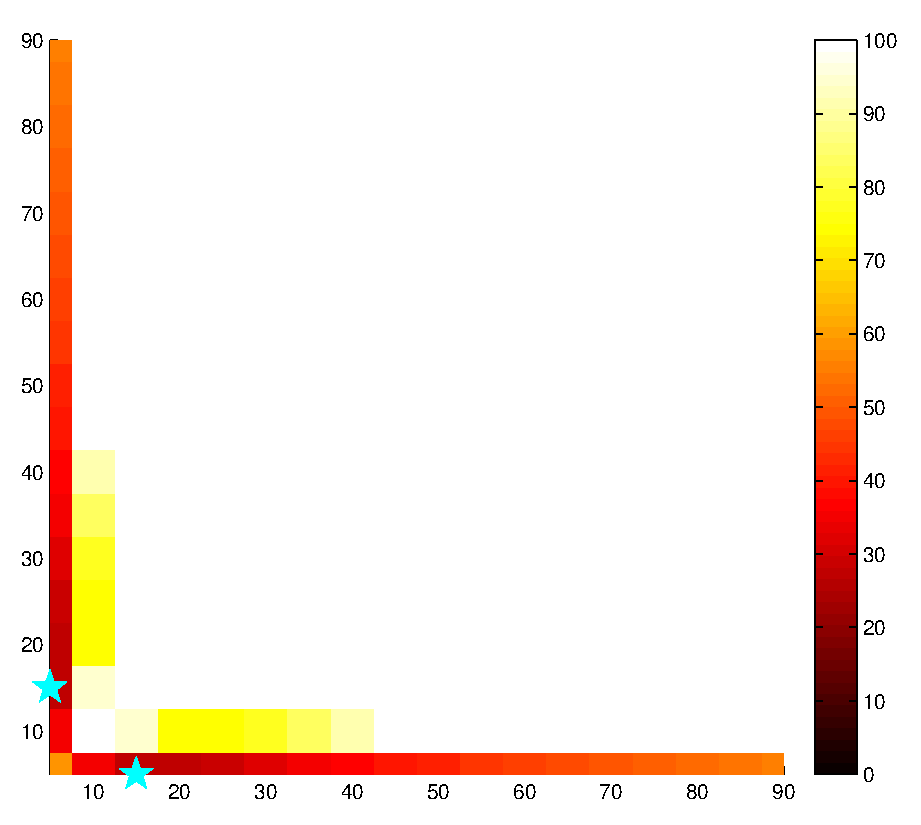
\includegraphics [height=3.41cm] {sigw_t1_vs_s1s2_21_41p90ms_0p1_1.eps}
				\label{fig:sigw,t1,s1s2,21}
			}
			\subfigure [$\sigwot$ vs. $(\alpha_1^\mathrm{spgr}, \alpha^\mathrm{dess})$] {
				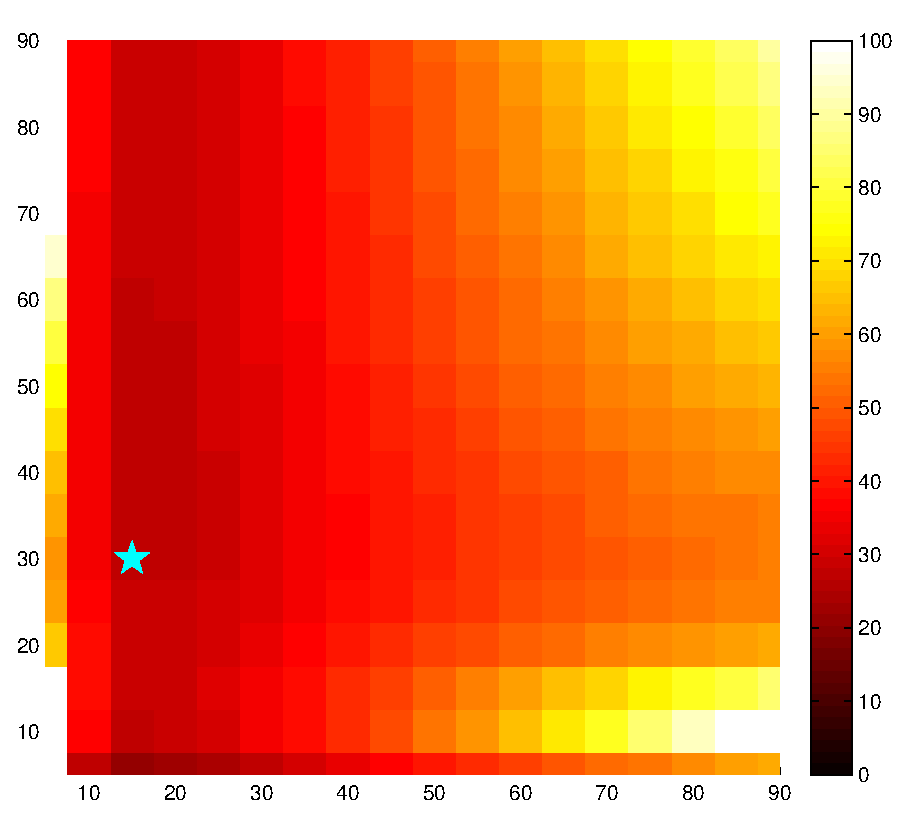
\includegraphics [height=3.41cm] {sigw_t1_vs_s1d1_21_41p90ms_0p1_1.eps}
				\label{fig:sigw,t1,s1d1,21}
			}
			\subfigure [$\sigwot$ vs. $(\alpha_2^\mathrm{spgr}, \alpha^\mathrm{dess})$] {
				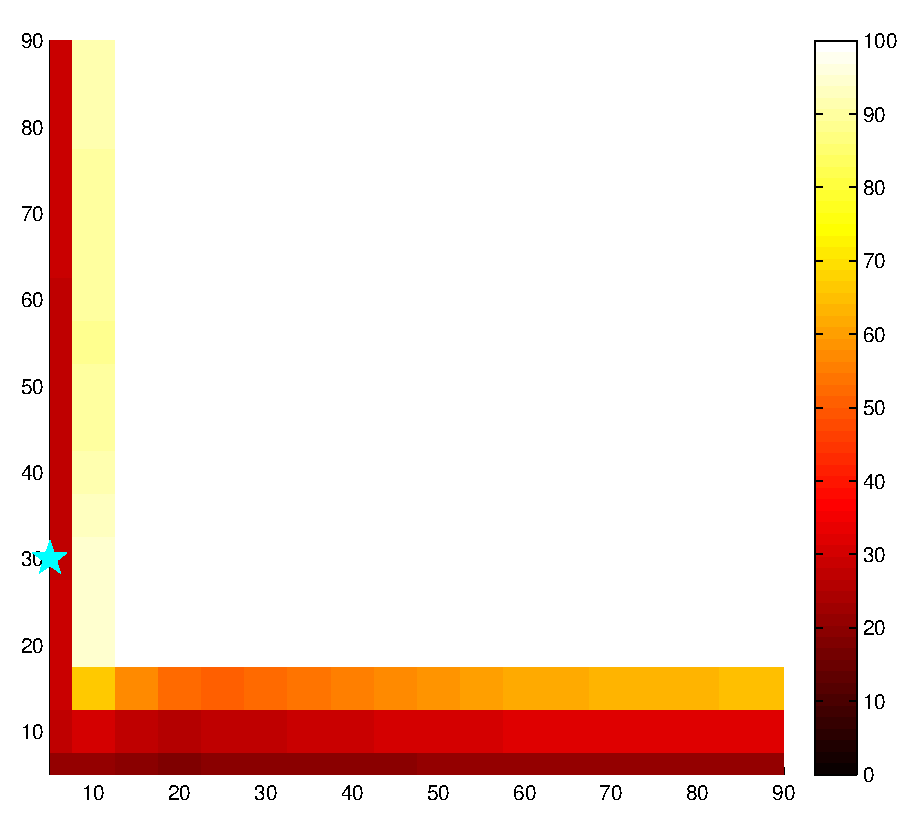
\includegraphics [height=3.41cm] {sigw_t1_vs_s2d1_21_41p90ms_0p1_1.eps}
				\label{fig:sigw,t1,s2d1,21}
			}
			
			\subfigure [$\sigwtt$ vs. $(\alpha_1^\mathrm{spgr}, \alpha_2^\mathrm{spgr})$] {
				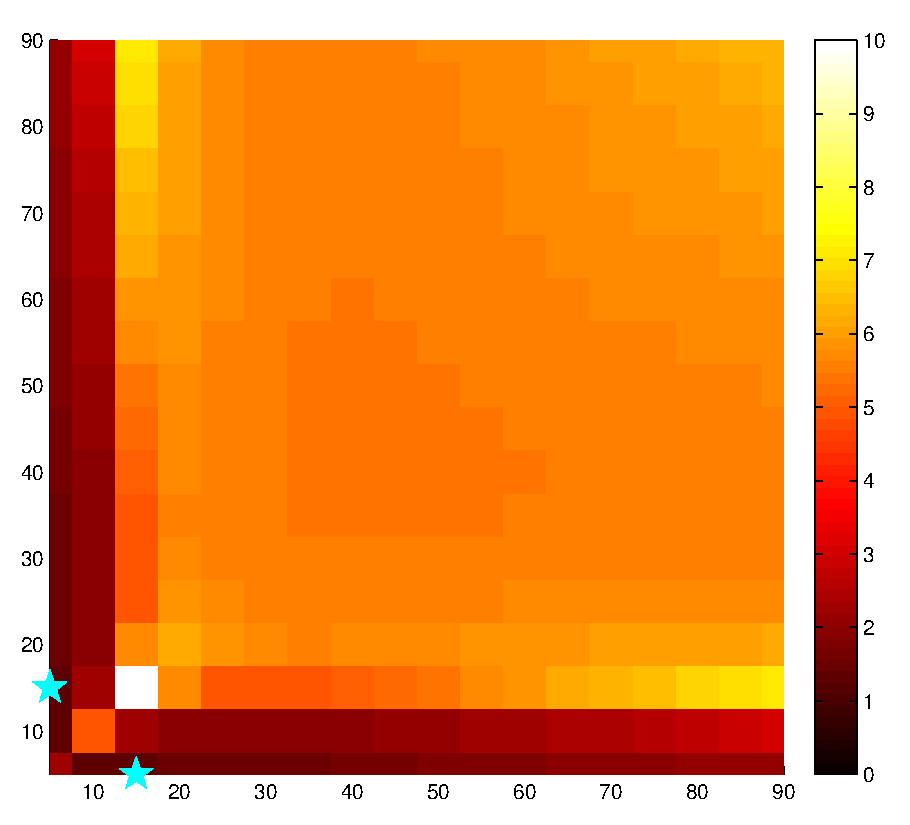
\includegraphics [height=3.41cm] {sigw_t2_vs_s1s2_21_41p90ms_0p1_1.eps}
				\label{fig:sigw,t2,s1s2,21}
			}
			\subfigure [$\sigwtt$ vs. $(\alpha_1^\mathrm{spgr}, \alpha^\mathrm{dess})$] {
				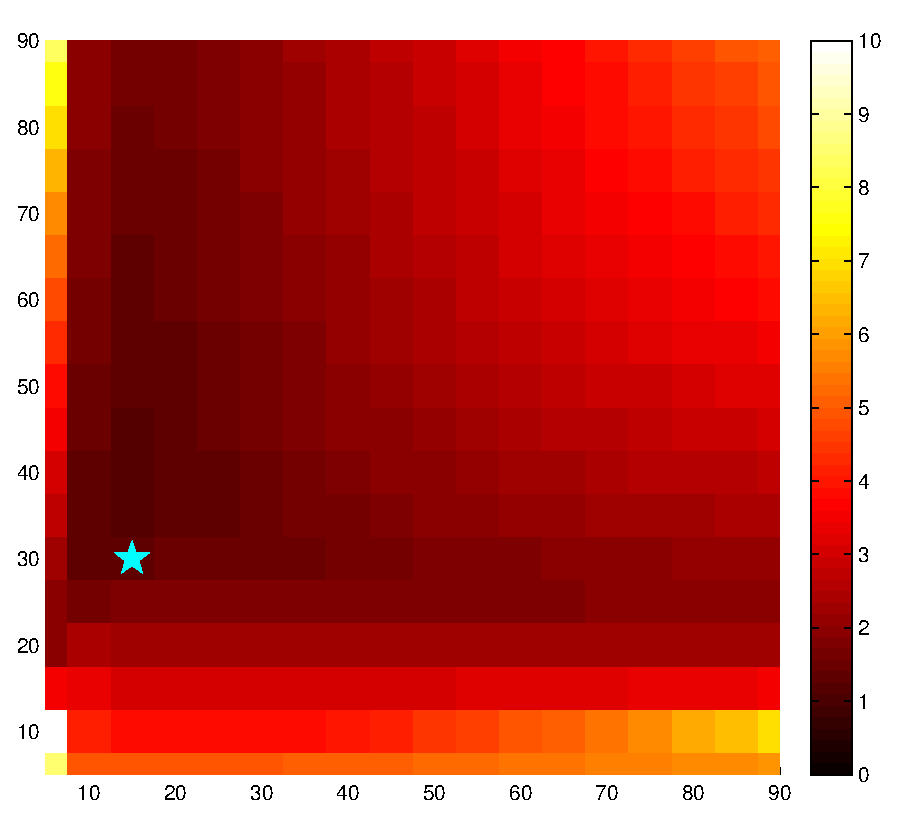
\includegraphics [height=3.41cm] {sigw_t2_vs_s1d1_21_41p90ms_0p1_1.eps}
				\label{fig:sigw,t2,s1d1,21}
			}
			\subfigure [$\sigwtt$ vs. $(\alpha_2^\mathrm{spgr}, \alpha^\mathrm{dess})$] {
				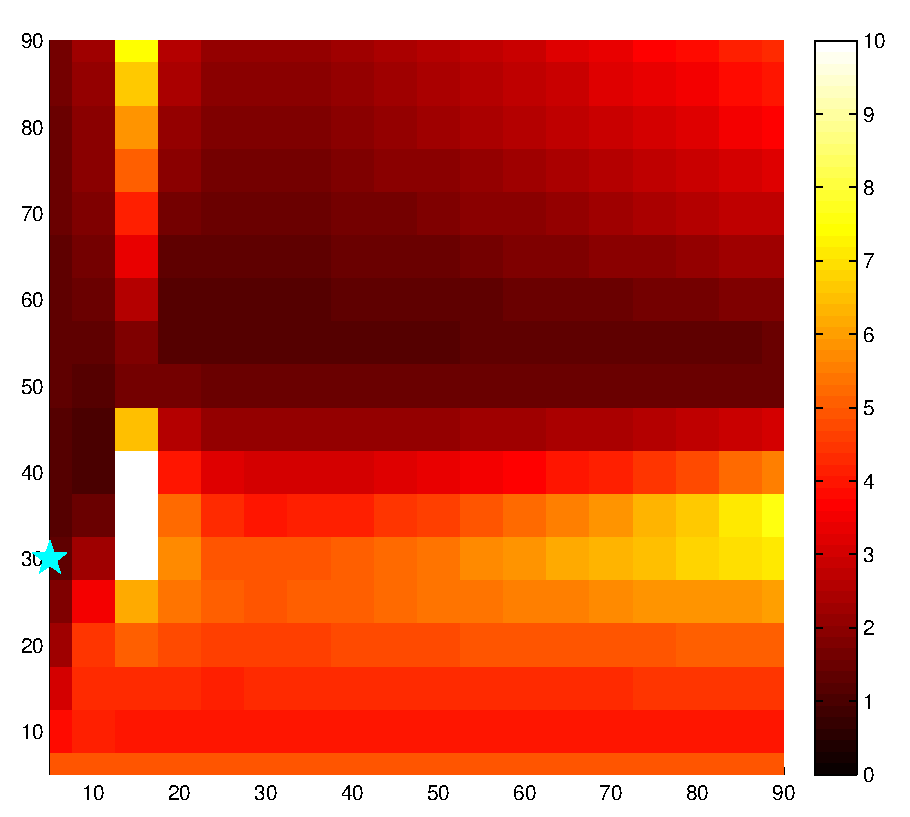
\includegraphics [height=3.41cm] {sigw_t2_vs_s2d1_21_41p90ms_0p1_1.eps}
				\label{fig:sigw,t2,s2d1,21}
			}
			
			\subfigure [$\costwt$ vs. $(\alpha_1^\mathrm{spgr}, \alpha_2^\mathrm{spgr})$] {
				\includegraphics [height=3.41cm] {Psiw_vs_s1s2_21_41p90ms_0p1_1.eps}
				\label{fig:sigw,t1,s1s2,21}
			}
			\subfigure [$\costwt$ vs. $(\alpha_1^\mathrm{spgr}, \alpha^\mathrm{dess})$] {
				\includegraphics [height=3.41cm] {Psiw_vs_s1d1_21_41p90ms_0p1_1.eps}
				\label{fig:sigw,t1,s1d1,21}
			}
			\subfigure [$\costwt$ vs. $(\alpha_2^\mathrm{spgr}, \alpha^\mathrm{dess})$] {
				\includegraphics [height=3.41cm] {Psiw_vs_s2d1_21_41p90ms_0p1_1.eps}
				\label{fig:sigw,t1,s2d1,21}
			}
		\end{minipage}
	}
	\fbox{ 
		\begin {minipage} [b] [12.5cm] [b] {0.18\textwidth}
			\subfigure [$\sigwot$ vs. $(\alpha^\mathrm{spgr}, \alpha^\mathrm{dess})$] {
				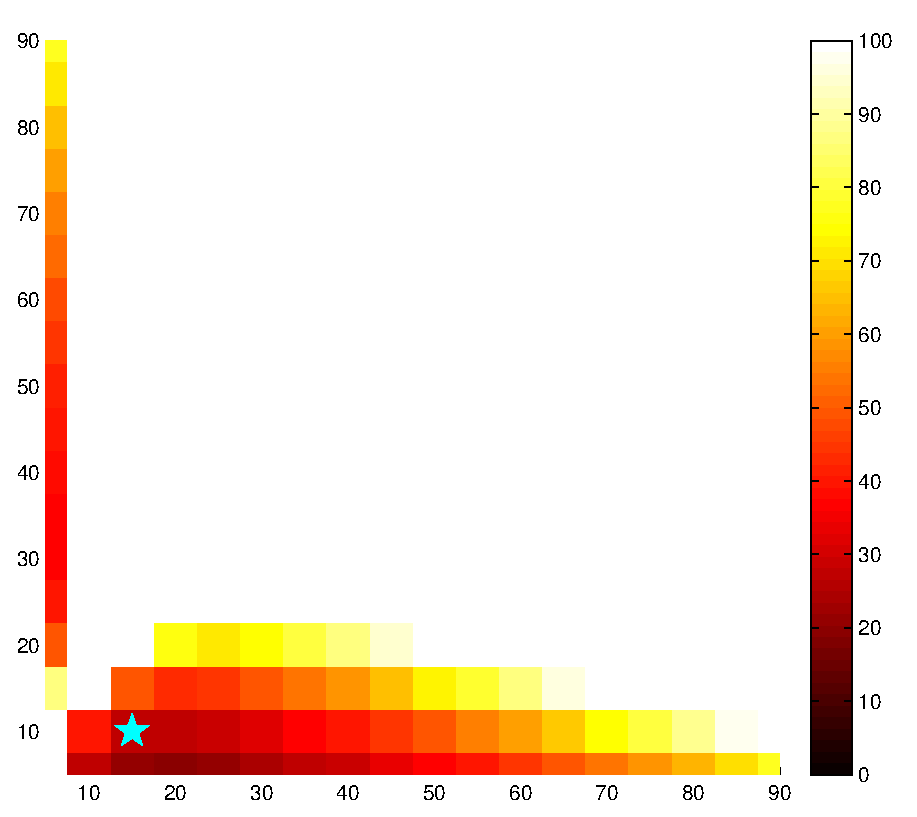
\includegraphics [height=3.41cm] {sigw_t1_vs_s1d1_11_41p90ms_0p1_1.eps}
				\label{fig:sigw,t1,s1d1,11}
			}
			
			\subfigure [$\sigwtt$ vs. $(\alpha^\mathrm{spgr}, \alpha^\mathrm{dess})$] {
				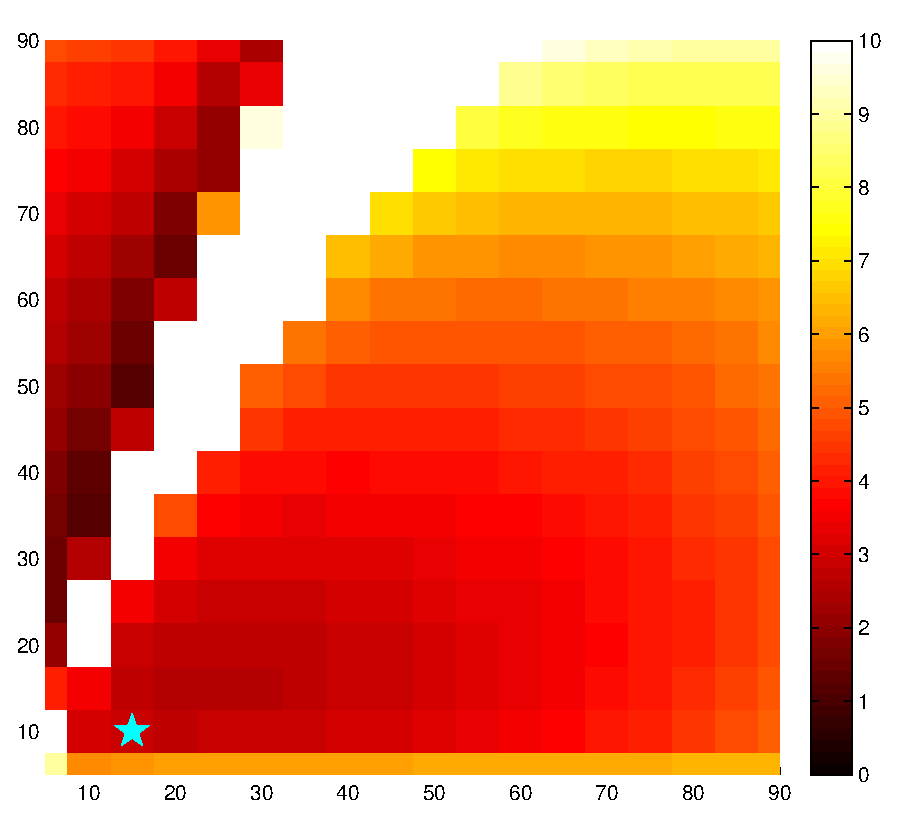
\includegraphics [height=3.41cm] {sigw_t2_vs_s1d1_11_41p90ms_0p1_1.eps}
				\label{fig:sigw,t2,s1d1,11}
			}
			
			\subfigure [$\costwt$ vs. $(\alpha^\mathrm{spgr}, \alpha^\mathrm{dess})$] {
				\includegraphics [height=3.41cm] {Psiw_vs_s1d1_11_41p90ms_0p1_1.eps}
				\label{fig:Psiw,s1d1,11}
			}
		\end{minipage}	
	}
	\fbox{ 
		\begin {minipage} [b] [12.5cm] [b] {0.18\textwidth}
			\subfigure [$\sigwot$ vs. $(\alpha_1^\mathrm{dess}, \alpha_2^\mathrm{dess})$] {
				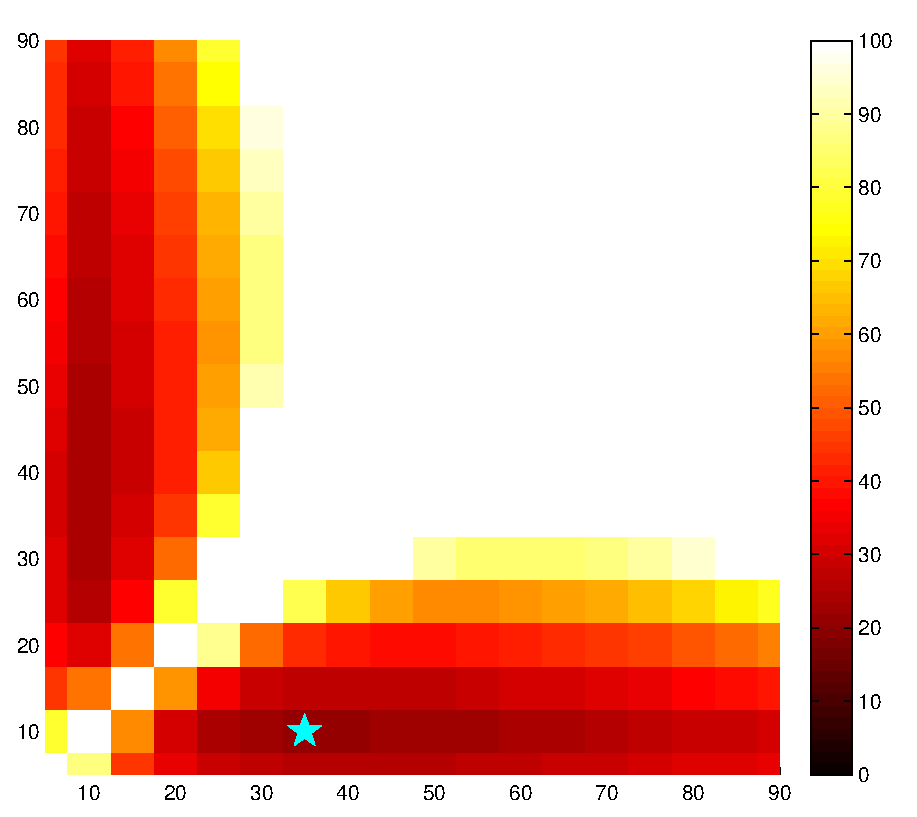
\includegraphics [height=3.41cm] {sigw_t1_vs_d1d2_02_41p90ms_0p1_1.eps}
				\label{fig:sigw,t1,d1d2,02}
			}
			
			\subfigure [$\sigwtt$ vs. $(\alpha_1^\mathrm{dess}, \alpha_2^\mathrm{dess})$] {
				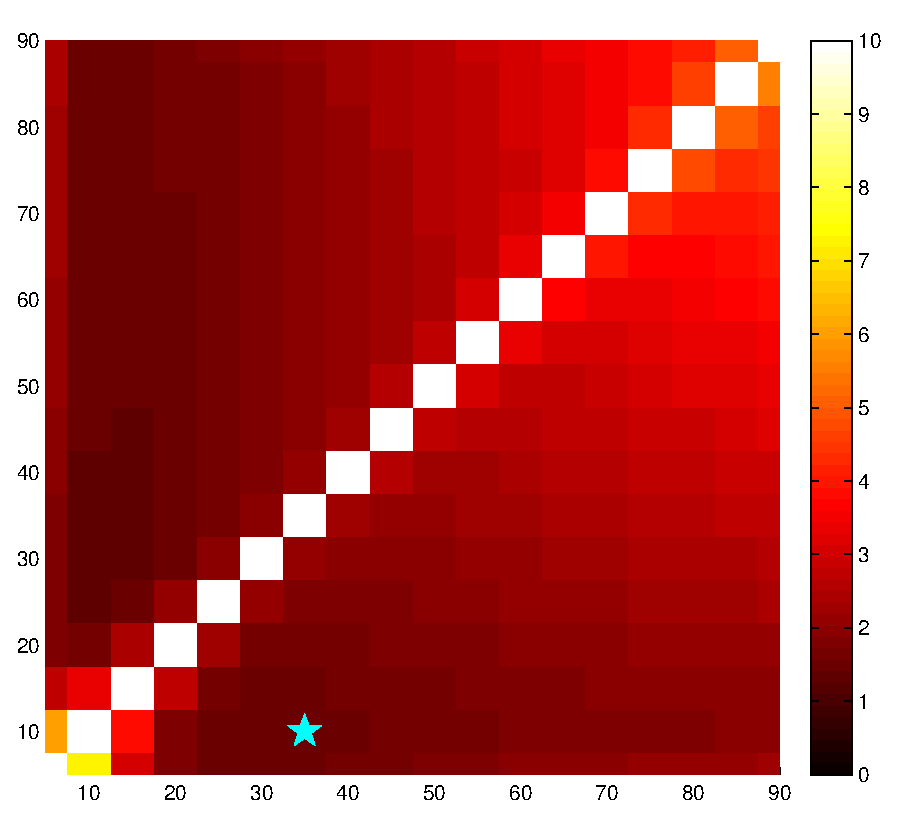
\includegraphics [height=3.41cm] {sigw_t2_vs_d1d2_02_41p90ms_0p1_1.eps}
				\label{fig:sigw,t2,d1d2,02}
			}
			
			\subfigure [$\costwt$ vs. $(\alpha_1^\mathrm{dess}, \alpha_2^\mathrm{dess})$] {
				\includegraphics [height=3.41cm] {Psiw_vs_d1d2_02_41p90ms_0p1_1.eps}
				\label{fig:Psiw,d1d2,02}
			}
		\end{minipage}	
	}
	\caption{
		Worst-case standard deviations $\sigwot$ (top), $\sigwtt$ (middle), and cost $\costwt$ (bottom), versus pairs of nominal flip angles, holding other scan parameters fixed at selected profile $\bmPs$. 
		Subfigures (a)-(i), (j)-(l), and (m)-(o) correspond to scan profiles containing $(\Ss, \Sd) = (2,1), (1,1), \text{and}\,(0,2)$ SPGR and DESS scans, respectively. 
		Selected scan parameters (starred) are within $\delta = 1$\% of global minimizers and retain as much estimator precision as possible over a wide range of latent object parameters. 		
		All axes range from 5 to 90 degrees, in 5-degree increments. 
		Colorbar ranges are $[0,100]$, $[0,10]$, and $[0,20]$ milliseconds for rows of $\sigwot$, $\sigwtt$, and $\costwt$ subfigures, respectively. 
		The optimized $(0,2)$ profile appears most robust to transmit field spatial variation.
	}
	\label{fig:heat,maps}
\end{sidewaysfigure}

Fig.~\ref{fig:heat,maps} displays heat maps 
of worst-case latent parameter standard deviations 
$\sigwot$, $\sigwtt$ 
and worst-case cost $\costwt$ 
as pairs of flip angles are varied away 
from the optimized scan design $\bmPs$.
Boxes group subfigures corresponding 
to the same scan profile. 
Viewing the bottom row of subfigures, 
it is evident 
that $\costwt(\bmPs)$ takes similar values 
for the different scan profiles. 
However, 
it is apparent that the $(\Ss,\Sd) = (0,2)$ profile 
is substantially more robust 
to transmit field variation 
than other tested profiles 
(namely, $(2,1)$ and $(1,1)$). 
Optimized worst-case cost 
over broadened latent parameter ranges 
$\costwb(\bmPs)$ captures this 
by expanding the range of possible flip angles 
from $\setNt = [0.9, 1.1]$ to $\setNb = [0.5, 2]$ 
to account for factor-of-two spatial variation 
in relative flip angle.
As a result, we find that the properties 
of ``broad'' search criterion $\costwb$ 
provide a stronger reason to select the $(0,2)$ scan 
for joint $\To, \Tt$ estimation in the brain 
than the properties 
of ``tight'' search criterion $\costwt$.

As the DESS sequence has already found success 
for $\Tt$ mapping from even one scan \cite{welsch:09:reo}, 
it is reassuring but unsurprising that our analysis finds two DESS scans 
to yield the most precise $\Tt$ estimates. 
More interestingly, 
our methods suggest that, 
with a minimum $\Sd = 2$ scans, 
DESS can be used to simultaneously estimate $\To$ as well. 
In fact, for certain choices of parameter ranges, 
a second DESS scan is predicted 
to afford $\widehat{T}_1$ precision 
comparable to two SPGR scans. 

%%%%%%%%%%%%%%%%%%%%%%%%%%%%%%%%%%%%%%%%%%%%%%%%%%%
\section{Experimental Validation and Results}
\label{s,scn-dsgn,exp}
%%%%%%%%%%%%%%%%%%%%%%%%%%%%%%%%%%%%%%%%%%%%%%%%%%%

To test our approach 
to optimized scan design 
(described in Section~\ref{ss,scn-dsgn,crb,minmax}), 
we estimate $\bmTo$ and $\bmTt$ maps 
(using maximum likelihood (ML) and 
regularized likelihood (RL) methods 
detailed in Section~\ref{ss,relax,meth,est}) 
from datasets collected 
using the scan profiles 
optimized in Section~\ref{s,scn-dsgn,opt}. 
In Section~\ref{ss,scn-dsgn,exp,sim}, 
we study estimator statistics from simulated data.
In Sections~\ref{ss,scn-dsgn,exp,phant}-\ref{ss,scn-dsgn,exp,invivo}, 
we progress to phantom and \emph{in vivo} datasets 
to evaluate scan profile performance 
under increasingly complex settings.
For the latter experiments, 
we use reference parameter maps 
from classical (long) pulse sequences, 
in lieu of ground truth maps.

%%%%%%%%%%%%%%%%%%%%%%%%%%%%%%%%%%%%%%%%%%%%%%%%%%%
\subsection{Numerical Simulations}
\label{ss,scn-dsgn,exp,sim}

We select $\To$ and $\Tt$ WM and GM values 
based on previously reported measurements 
at 3T \cite{wansapura:99:nrt, stanisz:05:ttr} 
and extrapolate other nuisance latent object parameters 
$\mzero$ and $\Tts$
from measurements at 1.5T \cite{kwan:99:msb}. 
We assign these parameter values
to the discrete anatomy 
of the BrainWeb digital phantom 
\cite{collins:98:dac, kwan:99:msb} 
to create ground truth $\bmMz, \bmTo, \bmTt, \bmTts \in \reals{V}$ maps. 
We then choose acquisition parameters based 
on Table~\ref{table:profile} 
(with fixed $\TE~=~4.67$ms) 
and apply models \eqref{eq:spgr-model} 
and \eqref{eq:dess-def-model}-\eqref{eq:dess-ref-model} 
to the 81st slices of these true maps 
to compute noiseless $217 \times 181$ SPGR and DESS image-domain data, 
respectively. 

For each scan profile, 
we corrupt the corresponding (complex) noiseless dataset $\bmS$ 
with additive complex Gaussian noise, 
whose variance $\sigma^2 \gets 1.49 \times 10^{-7}$ 
is set to match CRB calculations. 
This yields realistically noisy datasets $\bmY$ ranging 
from 105-122 signal-to-noise ratio (SNR), 
where SNR is defined here as
\begin{align}
	\snr{\bmS,\bmY} := \frac{\frob{\bmS}}{\frob{\bmY-\bmS}}.
	\label{eq:snr}
\end{align}
We use each profile's noisy magnitude dataset $\abs{\bmY}$
to compute estimates $\bmToest$ and $\bmTtest$ 
We then evaluate estimator bias and variance 
from latent ground truth $\bmTo$ and $\bmTt$ maps.

In these simulations, 
we intentionally neglect to model 
a number of physically realistic effects 
because their inclusion 
would complicate study of estimator statistics. 
First and foremost, 
we assume knowledge 
of a uniform  transmit field, 
to avoid confounding $\stx$ and $\To, \Tt$ estimation errors. 
For a similar reason, 
spatial variation in the sensitivity 
of a single receive coil is also not considered. 
We omit modeling partial volume effects 
to ensure deterministic knowledge of WM and GM ROIs. 
We will explore the influence of these (and other) nuisance effects 
on scan design in later subsections and chapters. 

To isolate bias due to estimator nonlinearity 
from regularization bias, 
we solve ML problem \eqref{eq:relax,ml-est} only,
and do not proceed to solve RL problem \eqref{eq:relax,rl-est}.
This permits consideration of $\To,\Tt$ estimation 
from each of the 7733 WM or 9384 GM data points 
as voxel-wise independent realizations 
of the same estimation problem. 
To minimize quantization bias, 
we optimize \eqref{eq:relax,ml-est} using a finely spaced dictionary 
of signal vectors from 1000 $\To$ and $\Tt$ values 
logarithmically spaced between 
$[10^2, 10^{3.5}]$ and $[10^1, 10^{2.5}]$, respectively. 
Using $10^6$ dictionary elements, 
solving \eqref{eq:relax,ml-est} took less than 7 minutes 
for each tested scan design $\bmPs$.

% T1/T2 simulation summary table
\begin{table} [!tb]
	\centering
	{\tabulinesep = 0.2mm
	\begin{tabu} {c | r r r | r}
		\hline \hline
		Scan 		& $(2,1)$ 			& $(1,1)$ 			& $(0,2)$			& Truth \\
		\hline
		WM $\ToML$	& $830 \pm 17$		& $830 \pm 15$		& $830 \pm 14$		& $832$	\\
		GM $\ToML$ 	& $1330 \pm 30.$	& $1330 \pm 24$		& $1330 \pm 24$		& $1331$ \\
		\hline
		WM $\TtML$ 	& $80. \pm 1.0$		& $80. \pm 2.1$		& $79.6 \pm 0.94$	& $79.6$ \\
		GM $\TtML$	& $110. \pm 1.4$	& $110. \pm 3.0$	& $110. \pm 1.6$ 	& $110$ \\
		\hline \hline
	\end{tabu}}
	\vspace{1mm}
	\caption{Sample means $\pm$ sample standard deviations of $\bmTo$ and $\bmTt$ ML estimates in WM and GM ROIs of simulated data, compared across different optimized scan profiles. Sample means exhibit insignificant bias, and sample standard deviations are consistent with worst-case standard deviations $\sigwot$ and $\sigwtt$ reported in Table \ref{table:profile}. All values are reported in milliseconds.}
	\label{table:numerical}
\end{table}

Table~\ref{table:numerical} verifies
\footnote{Each sample statistic presented 
in this chapter 
is rounded off to the highest place value 
of its corresponding uncertainty measure.
For simplicity, 
each uncertainty measure is itself endowed 
one extra significant figure.
Decimal points indicate the significance of trailing zeros.
}	
that, 
despite model nonlinearity and Rician noise,
estimation bias in WM- and GM-like voxels is negligible.
Sample standard deviations are consistent with $\sigwot$ and $\sigwtt$ (\emph{cf.}~Table~\ref{table:profile}). 
We observe that the $(1,1)$ and $(0,2)$ profiles afford high 
$\bmToest^\mathrm{ML}$ precision, 
while the $(2,1)$ and $(0,2)$ scans afford high 
$\bmTtest^\mathrm{ML}$ precision. 
In agreement with the predictions 
of $\costwt$ and $\costwb$, 
these simulation studies suggest that at these SNR levels,
an optimized profile containing 2 DESS scans
can permit $\bmTo$ and $\bmTt$ estimation precision 
in WM and GM comparable to optimized profiles 
containing SPGR/DESS combinations.
	
% Simulation T1/T2 distributions for (0,2) scan
\begin{figure} [!tbp]
	\centering
	\subfigure [$\ToML$ in voxels with WM-like $\To \gets 832$] {
		\includegraphics [width = 0.43\textwidth] {T1_hist_ml_wm_3parm_0SPGR2DESS.eps}
		\label{fig:t1,hist,wm,02}
	}
	\hspace{1cm}
	\subfigure [$\ToML$ in voxels with GM-like $\To \gets 1331$] {
		\includegraphics [width = 0.43\textwidth] {T1_hist_ml_gm_3parm_0SPGR2DESS.eps}
		\label{fig:t1,hist,gm,02}
	}
	\vspace{0.2cm}
	
	\subfigure [$\TtML$ in voxels with WM-like $\Tt \gets 79.6$] {
		\includegraphics [width = 0.43\textwidth] {T2_hist_ml_wm_3parm_0SPGR2DESS.eps}
		\label{fig:t2,hist,wm,02}
	}
	\hspace{1cm}
	\subfigure [$\TtML$ in voxels with GM-like $\Tt \gets 110$] {
		\includegraphics [width = 0.43\textwidth] {T2_hist_ml_gm_3parm_0SPGR2DESS.eps}
		\label{fig:t2,hist,gm,02}
	}
	\caption{
		Histograms of $\To$ and $\Tt$ estimates 
		from noisy independent measurements 
		of a \emph{single} nominal WM or GM value. 
		In each plot, two normal distributions are overlaid, 
		each with latent means $\To$ and $\Tt$. 
		In (a)-(b) and (c)-(d), the solid green curve 
		is $\gauss{\To}{(\sigwot)^2)}$ 
		and $\gauss{\Tt}{(\sigwtt)^2}$, respectively.
		In (a)-(d), the dashed maroon curves have variances computed 
		from the Fisher information at \emph{a priori} unknown $\To, \Tt$ values 
		in WM or GM. 
		These plots correspond to an optimized $(0,2)$ scan profile; 
		analogous plots for other profiles are visually similar. 
		At realistic noise levels,
		parameter estimates distribute 
		with minimal bias and near-Gaussian shape.
		Thus, the CRB reliably approximates 
		$\ToML$ and $\TtML$ errors.
	}
	\label{fig:normality}
\end{figure}

Fig.~\ref{fig:normality} histograms (voxel-wise independent) ML estimates 
$\widehat{T}_1^{\mathrm{ML}}$ and $\widehat{T}_2^{\mathrm{ML}}$ 
from the $(0,2)$ scan profile.
Each histogram is over a WM or GM ROI, 
within which all voxels are assigned 
the same single-component true $\To$ and $\Tt$ nominal value, 
listed in Table~\ref{table:numerical}.

Overlaid in dashed maroon are normal distributions 
with latent means $\To$ and $\Tt$ 
and variances computed 
from the Fisher matrix at $\To,\Tt$ values 
in WM or GM. 
It is apparent that despite finite SNR and Rician noise, 
$\widehat{T}_1^{\mathrm{ML}}$ and $\widehat{T}_2^{\mathrm{ML}}$ 
exhibit negligible bias and near-Gaussian shape, 
suggesting locally linear behavior of the DESS signal model 
in $\To$ and $\Tt$ 
($\widehat{T}_1^{\mathrm{ML}}$ and $\widehat{T}_2^{\mathrm{ML}}$ distributions 
from other profiles are similar). 

% tradeoff: bigger range of interest, further from optimal variance 
The subfigures of Fig.~\ref{fig:normality} superimpose 
in solid green a second set of normal distributions, 
with the same means $\To$ and $\Tt$ as before, 
but worst-case standard deviations $\sigwot$ and $\sigwtt$. 
The separations between these distribution pairs 
visually depict how estimator variances specific 
to WM or GM $\To$ and $\Tt$ values differ 
from worst-case variances. 
Using the fixed latent object parameters 
to optimize scan profiles can tailor scans 
for precise estimation in \emph{either} WM \emph{or} GM. 
In contrast, the proposed min-max formulation finds scan parameters 
that ensure precise estimation 
in \emph{both} WM \emph{and} GM.	

%%%%%%%%%%%%%%%%%%%%%%%%%%%%%%%%%%%%%%%%%%%%%%%%%%%
\subsection{Phantom Experiments}
\label{ss,scn-dsgn,exp,phant}

This subsection describes two experiments. 
In the first experiment, 
we compare SPGR/DESS scan profiles 
described in Table~\ref{table:profile} 
(as well as a reference profile consisting of IR and SE scans) 
against nuclear magnetic resonance (NMR) measurements 
from the National Institute for Standards and Technology (NIST) 
\cite{keenan:16:msm}.
These measurements provide information 
about \emph{ROI sample means} and \emph{ROI sample standard deviations} 
(Fig.~\ref{fig:hpd,ml-rls}), 
which we define as first- and second-order statistics 
computed across voxels within an ROI.
In the second experiment, 
we repeat the SPGR/DESS scan profiles 10 times 
and compute \emph{sample standard deviation maps} 
across repetitions. 
Taking ROI sample means of these maps 
gives \emph{pooled sample standard deviations} 
(Table~\ref{table:hpd,sample-std-dev}), 
which indicate relative scan profile precision.

%%%%%%%%%%%%%%%%%%%%%%%%%%%%%%%%%%%%%%%%%%%%%%%%%%%	
\subsubsection{Within-ROI Statistics} 
\label{sss,scn-dsgn,exp,phant,roi}

We acquire combinations 
of $(2,1)$, $(1,1)$, and $(0,2)$ SPGR and DESS coronal scans 
of a High Precision Devices\regis MR system phantom $\Tt$ array.
For each scan profile, 
we prescribe the optimized flip angles $\bmflipnomest$ 
and repetition times $\bmTRest$ 
listed in Table~\ref{table:profile},
 and hold all other scan parameters fixed. 
We achieve the desired nominal flip angles 
by scaling a 20mm slab-selective Shinnar-Le Roux excitation \cite{pauly:91:prf}, 
of duration 1.28ms and time-bandwidth product 4. 
For each DESS (SPGR) scan, 
we apply 2 (10) spoiling phase cycles 
over a $5$mm slice thickness. 
We acquire all steady-state phantom and \emph{in vivo} datasets 
with a $256 \times 256 \times 8$ matrix 
over a $240 \times 240 \times 30$ mm$^3$ field of view (FOV). 
Using a 31.25kHz readout bandwidth, 
we acquire all data at minimum $\TE \gets 4.67$ms 
before or after RF excitations. 
To avoid slice-profile effects, 
we sample $\mathbf{k}$-space over a 3D Cartesian grid. 
After Fourier transform of the raw datasets, 
only one of the excited image slices 
is used for subsequent parameter mapping. 
Including time to reach steady-state, 
each steady-state scan profile requires 1m37s scan time.

To validate a reference scan profile 
for use in \emph{in vivo} experiments, 
we also collect 4 IR and 4 SE scans.
For (phase-sensitive, SE) IR, 
we hold $(\TR, \TE) \gets (1400, 14)$ms fixed 
and vary (adiabatic) inversion time 
$\TI \in \set{50, 150, 450, 1350}$ms across scans.
For SE, we similarly hold $\TR \gets 1000$ms fixed 
and vary echo time $\TE \in \set{10, 30, 60, 150}$ms across scans.
We prescribe these scan parameters 
to acquire $256 \times 256$ datasets 
over the same $240 \times 240 \times 5$ mm$^3$ slice processed 
from the SPGR/DESS datasets. 
Each IR and SE scan requires 5m58s and 4m16s, 
for a total 40m58s scan time.

We additionally collect a pair 
of Bloch-Siegert shifted 3D SPGR scans 
for separate transmit field estimation 
\cite{sacolick:10:bmb}. 
We insert a 9ms Fermi pulse 
at $\pm8$kHz off-resonance
into an SPGR sequence immediately following on-resonant excitation.
We estimate regularized transmit field maps \cite{sun:14:reo}
from the resulting pair of datasets.
We normalize this transmit field map estimate
by the 0.075G peak Fermi pulse amplitute
to estimate transmit coil spatial variation map $\bmstx$.
After calibration via separate measurements,
we take $\bmstx$ as known.
For consistency, we account for flip angle variation 
when estimating $\bmTo$ and $\bmTt$ 
from both candidate (SPGR/DESS) 
and reference (IR/SE) scan profiles.
With a repetition time of 21.7ms, 
this transmit field mapping acquisition requires 
1m40s total scan time.

We acquire all phantom datasets 
using a GE Discovery\tmark MR750 3.0T scanner 
with an 8-channel receive head array. 
We separately normalize and combine coil data 
from each scan profile using a natural extension 
of \cite{ying:07:jir} to the case of multiple datasets. 
For each optimized SPGR/DESS scan profile $\bmPs$, 
we pre-cluster known parameter maps $\bmN$ 
into 10 clusters using $k$-means++ \cite{arthur:07:kmt} 
and use each of the 10 cluster means 
to compute a corresponding dictionary 
of signal vectors from 300 $\To$ and $\Tt$ values 
logarithmically spaced between $[10^{1.5}, 10^{3.5}]$ 
and $[10^{0.5}, 10^3]$, respectively.
We then iterate over clusters 
and use each dictionary in conjunction 
with corresponding coil-combined magnitude image data 
to produce ML parameter estimates 
$\estaML{\bmX}{\bmN,\bmPs}$.
We subsequently solve RL problem \eqref{eq:relax,rl-est} 
with initialization $\estaML{\bmX}{\bmN,\bmPs}$ 
to obtain regularized estimates $\estaRL{\bmX}{\bmN,\bmPs}$ 
for each $\bmPs$. 
We design regularizer \eqref{eq:relax,reg} 
to encourage RL parameter estimates 
from different scan profiles 
to exhibit similar levels of smoothness.
Letting $l \in \set{1, 2, 3}$ enumerate latent object parameters 
$\bmTo$, $\bmTt$, and the proportionality constant, 
we choose mild regularization parameters 
$(\beta_1, \beta_2, \beta_3) := D \times (2^{-21}, 2^{-23}, 2^{-26})$ 
to scale with the number of datasets
and fix shape parameters
$(\gamma_1, \gamma_2, \gamma_3) := (2^{5} \textrm{ ms}, 2^{2} \textrm{ ms}, 2^{-2})$ 
to values on the order 
of anticipated standard deviations.
We iteratively update $\bmX$ until convergence criterion 
\begin{align}
	\frob{\iter{\bmX}{i}-\iter{\bmX}{i-1}} < 10^{-7} \frob{\iter{\bmX}{i}}
	\label{eq:conv,crit}
\end{align}
is satisfied. 
For all steady-state profiles tested, 
ML initializations and RL reconstructions 
of phantom datasets require less than
3m30s and 9s, respectively.

We next describe sequential
\footnote{
We initially attempted 
to circumvent sequential $\bmTo$, then $\bmTt$ estimation 
by instead jointly estimating $\bmMz$, $\bmTo$, $\bmTt$, and inversion efficiency 
from the IR and SE datasets together.
Even using magnitude data and signal models, 
this resulted in heavily biased parameter maps, 
possibly due to the dependence 
of adiabatic inversion efficiency 
on relaxation parameters \cite{frank:97:spe}.
}
$\bmTo$,
then $\bmTt$ estimation
from IR and SE reference scans.
We first jointly coil-combine
all 8-channel IR and SE phantom datasets 
to produce complex images.
We next estimate $\bmTo$ along 
with a (nuisance parameter) inversion efficiency map
via \eqref{eq:relax,ml-est} and \eqref{eq:relax,rl-est} 
from the 4 complex coil-combined IR images.
By using the same flip angle scaling map $\bmstx$ 
as is used for SPGR/DESS profiles, 
we estimate $\bmTo$ using a signal model similar
to one proposed in \cite{barral:10:arm},
which accounts for imperfect excitation/refocusing 
and imperfect inversion.
We then take both $\bmTo$ and $\bmstx$ 
as known and estimate $\bmTt$ 
along with nuisance parameter $\bmMz$ 
(accounting for imperfect excitation/refocusing and incomplete recovery) 
via \eqref{eq:relax,ml-est} and \eqref{eq:relax,rl-est} 
from the 4 complex coil-combined SE images.
We hold all other reconstruction details identical 
to those of SPGR/DESS reconstructions.

% nist t1/t2 maps, jet
\begin{figure*} [!tb]
	\centering
	\subfigure{
		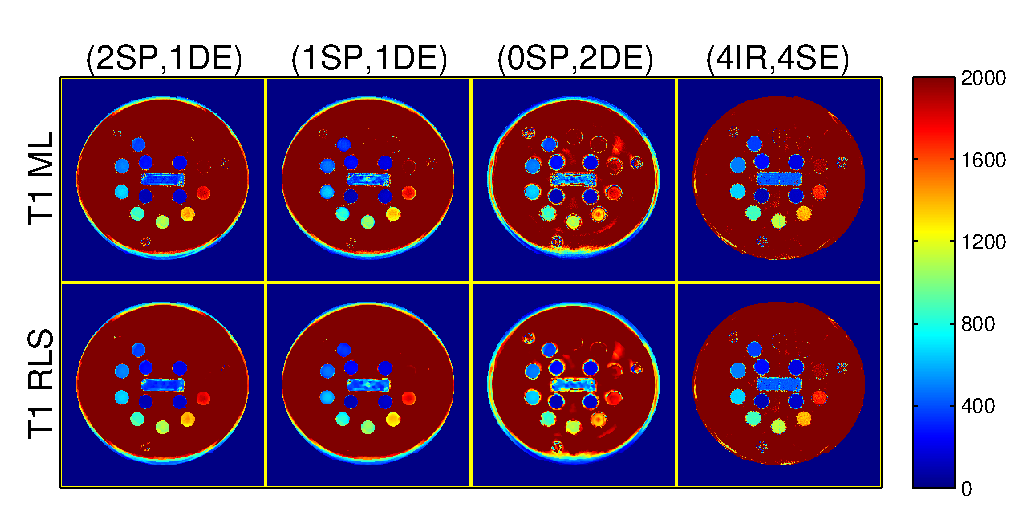
\includegraphics [width=15.4cm] {2016-06-20,hpd,t1,jet.eps}
		\label{fig:hpd,t1,jet}
	}
	\vspace{0cm}
	\subfigure{
		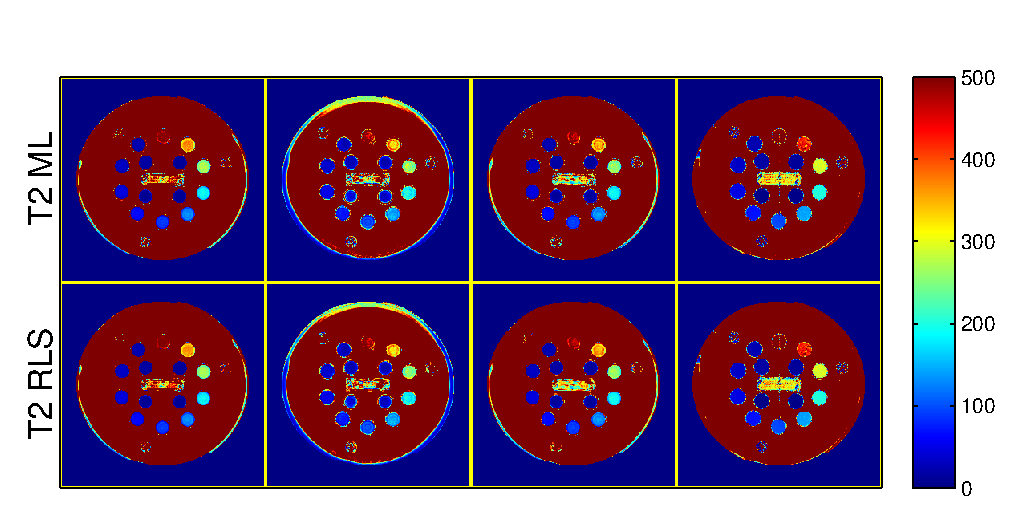
\includegraphics [width=15.2cm, trim=0 0 0 25, clip] {2016-06-20,hpd,t2,jet.eps}
		\label{fig:hpd,t2,jet}
	}
	\caption{
		Colorized $\bmTo$ and $\bmTt$ ML and RL estimates 
		from an HPD\regis quantitative phantom.
		Columns correspond to scan profiles consisting of 
		(2 SPGR, 1 DESS), (1 SPGR, 1 DESS), (0 SPGR, 2 DESS),
		and (4 IR, 4 SE) acquisitions. 
		Rows distinguish $\bmTo$ and $\bmTt$ ML and RL estimators. 
		Fig.~\ref{fig:hpd,gray} provides identical grayscale images
		that enumerate vials.
		Colorbar ranges are in milliseconds.
	}
	\label{fig:hpd,jet}
\end{figure*}

% nist t1/t2 maps, gray
\begin{figure*} [!tb]
	\centering
	\subfigure{
		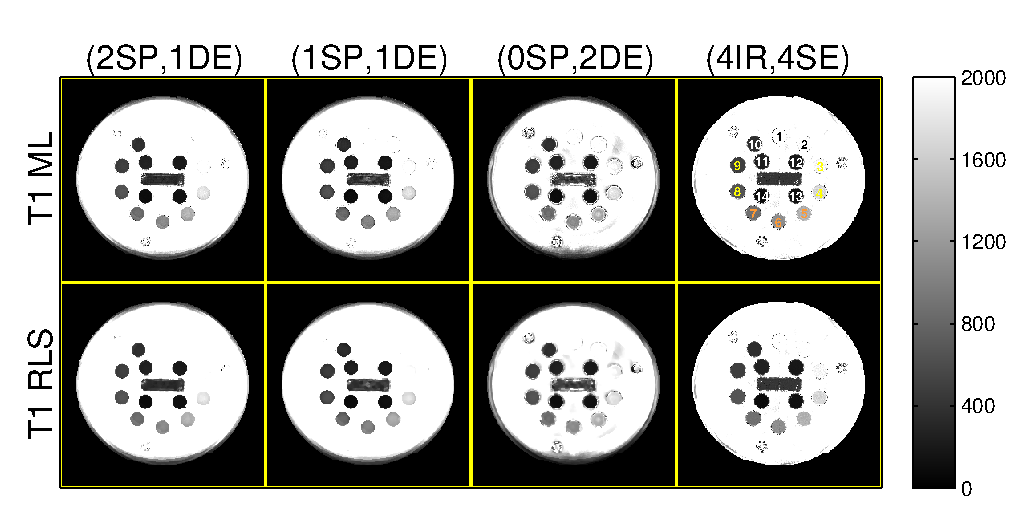
\includegraphics [width=15.4cm] {2016-06-20,hpd,t1,gray.eps}
		\label{fig:hpd,t1,gray}
	}
	\vspace{0cm}
	\subfigure{
		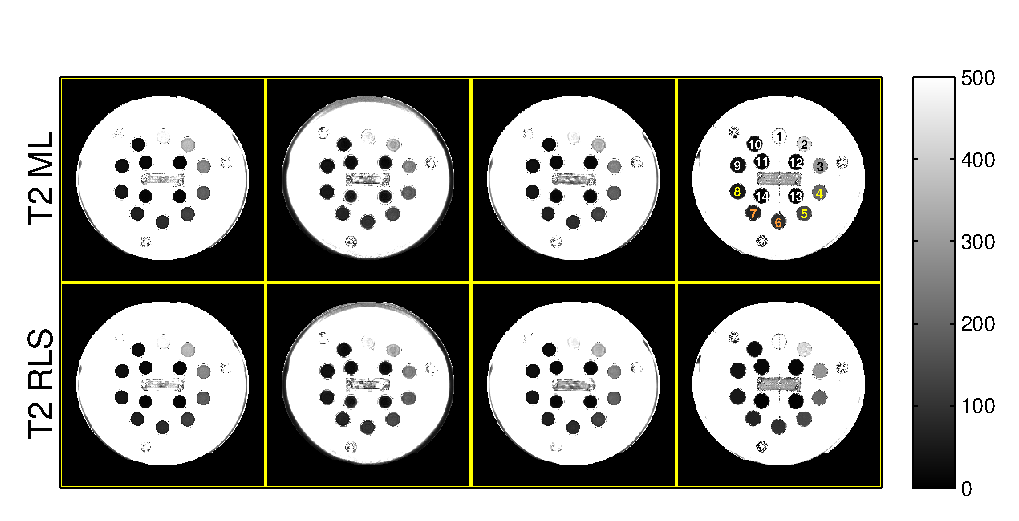
\includegraphics [width=15.2cm, trim=0 0 0 25, clip] {2016-06-20,hpd,t2,gray.eps}
		\label{fig:hpd,t2,gray}
	}
	\caption{
		Grayscale $\bmTo$ and $\bmTt$ ML and RL estimates 
		from an HPD\regis quantitative phantom.
		Columns correspond to scan profiles consisting of 
		(2 SPGR, 1 DESS), (1 SPGR, 1 DESS), (0 SPGR, 2 DESS),
		and (4 IR, 4 SE) acquisitions. 
		Rows distinguish $\bmTo$ and $\bmTt$ ML and RL estimators. 
		Vials are enumerated and color-coded
		to correspond with data points in Fig.~\ref{fig:hpd,ml-rls}.
		Fig.~\ref{fig:hpd,jet} provides identical colorized images.
		Colorbar ranges are in milliseconds.
	}
	\label{fig:hpd,gray}
\end{figure*}

Figs.~\ref{fig:hpd,jet}-\ref{fig:hpd,gray} compare
in color and grayscale  
phantom $\bmTo$ and $\bmTt$ ML and RL estimates 
from optimized scan profiles. 
Vials are enumerated 
in Fig.~\ref{fig:hpd,ml-rls} 
in descending $\To$ and $\Tt$ order. 
Vials corresponding to tight $\setXt$ 
and broad $\setXb$ parameter ranges are highlighted 
with orange and yellow labels, respectively. 
Within these vials of interest, 
parameter maps from different scans appear visually similar.

% outside range of interest, most severe bias in T1 ML (0,2) 
% appears that pure-DESS tends to have significantly greater systematic errors in regions of high T1 
In higher-$\To$ vials (and the surrounding water),
more bias is apparent 
in $\bmToest$ ML and RL estimates 
from the $(0,2)$ scan profile than 
from the $(2,1)$ and $(1,1)$ scan profiles. 
With the signal models used in this study,
the images suggest that scan profiles consisting 
of at least one SPGR scan may offer increased protection 
against $\To$ estimation bias.

% t1/t2 ml/rls hpd accuracy
\begin{figure*} [!tbp]
	\centering
	\subfigure [$\ToML$ Estimates] {
		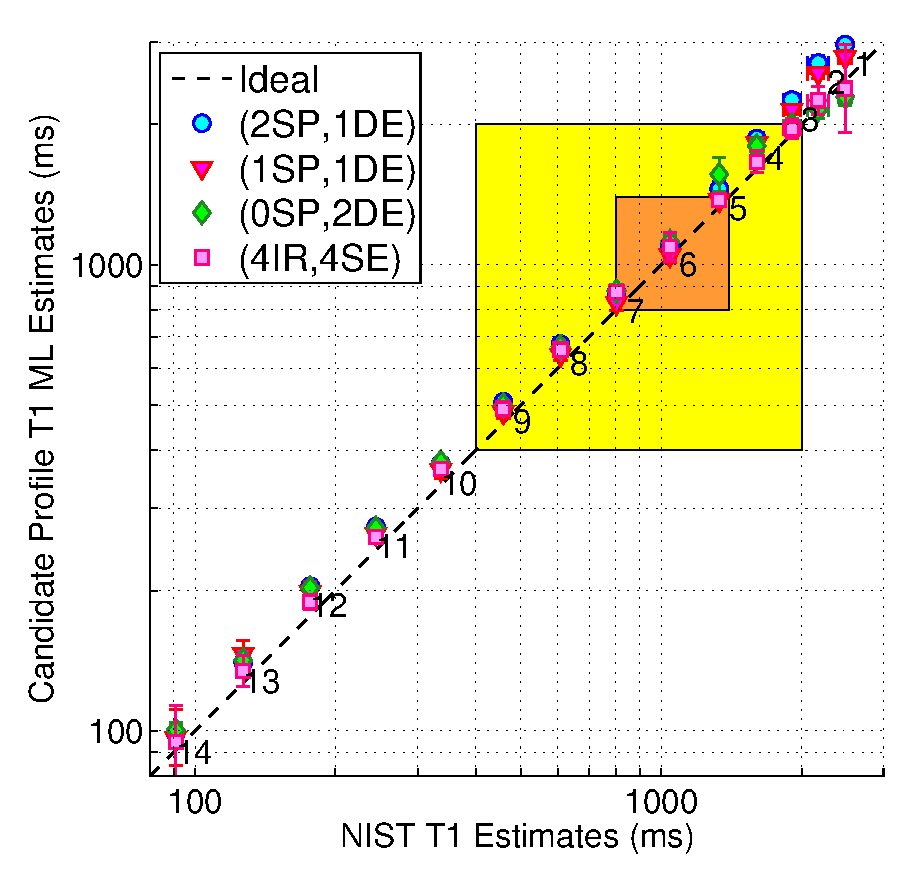
\includegraphics [width = 0.45\textwidth] {2016-06-20,hpd,t1-ml-compare.eps}
		\label{fig:t1,hpd,ml}
	}
	\hspace{0.3cm}
	\subfigure [$\TtML$ Estimates] {
		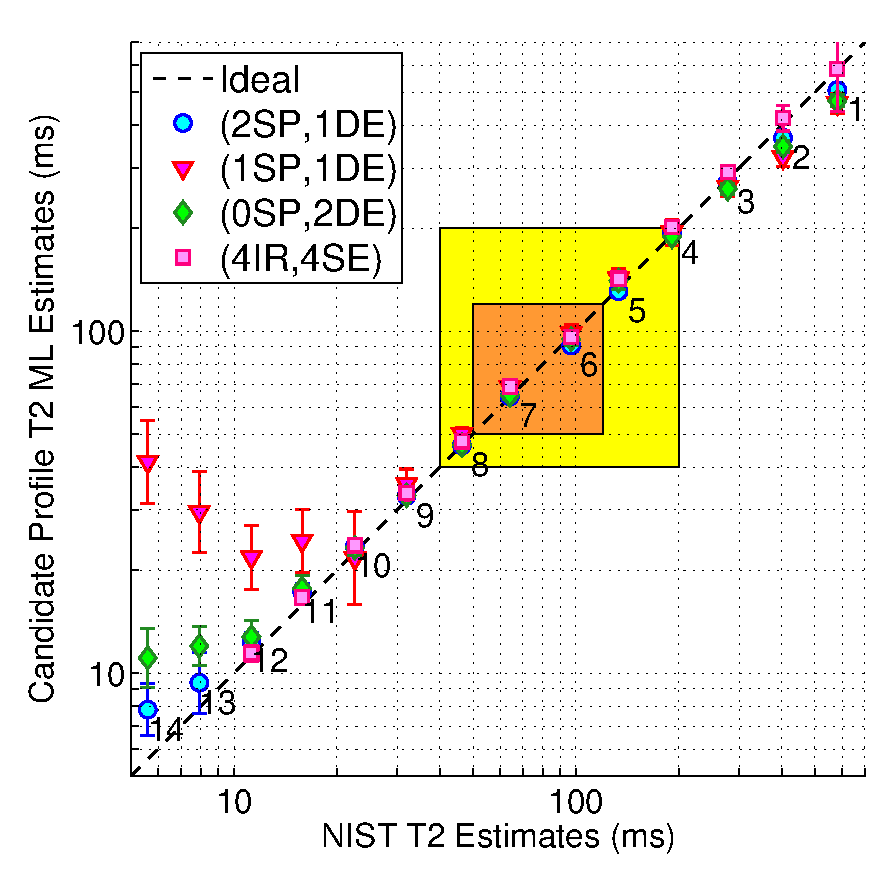
\includegraphics [width = 0.45\textwidth] {2016-06-20,hpd,t2-ml-compare.eps}
		\label{fig:t2,hpd,ml}
	}
	\vspace{-0.3cm}
	\subfigure [$\ToRL$ Estimates] {
		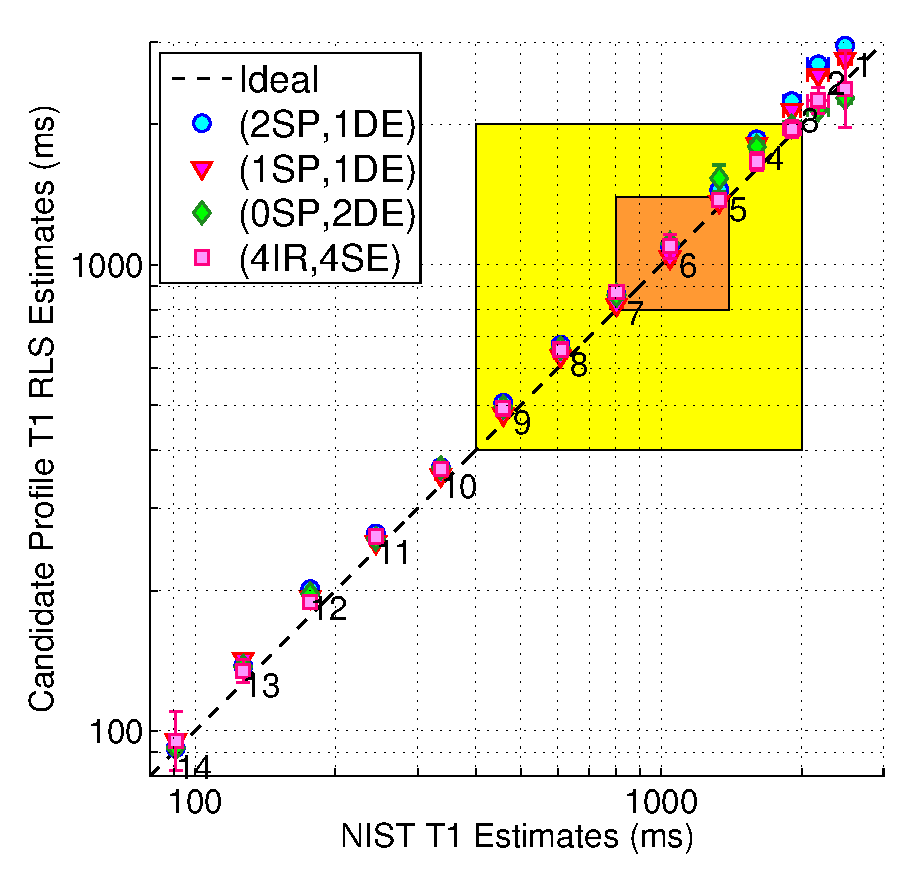
\includegraphics [width = 0.45\textwidth] {2016-06-20,hpd,t1-rls-compare.eps}
		\label{fig:t1,hpd,rls}
	}
	\hspace{0.3cm}
	\subfigure [$\TtRL$ Estimates] {
		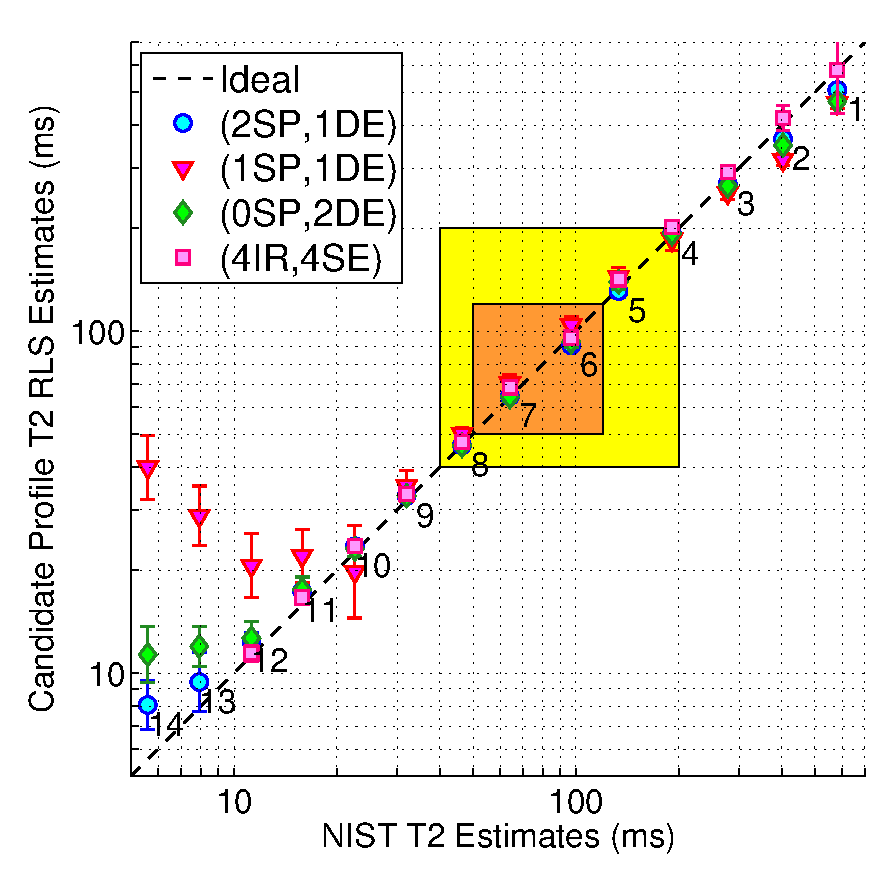
\includegraphics [width = 0.45\textwidth] {2016-06-20,hpd,t2-rls-compare.eps}
		\label{fig:t2,hpd,rls}
	}
	\caption{
		Phantom within-ROI sample statistics 
		of $\bmTo$ and $\bmTt$ ML and RL estimates 
		from optimized SPGR/DESS and reference IR/SE scan profiles, 
		versus NIST NMR measurements \cite{keenan:16:msm}.
		Markers and error bars indicate 
		ROI sample means and ROI sample standard deviations 
		within the 14 labeled and color-coded vials 
		in Fig.~\ref{fig:hpd,gray}.
		Tight $\setXt$ and broad $\setXb$ latent parameter ranges are highlighted 
		in orange and yellow, respectively.
		Table~\ref{table:hpd,accuracy} replicates sample statistics 
		within Vials 5-8.
		Our MR measurements are at 293K 
		and NIST NMR measurements are at 293.00K.
		Within the designed parameter ranges, 
		estimates from different acquisitions 
		are in reasonable agreement with NIST measurements.
	}
	\label{fig:hpd,ml-rls}
\end{figure*}

% t1/t2 ml/rls hpd accuracy-table
\begin{table*} [t]
	\centering
	\begin{tabu} {c || r r r | r || r}
		\hline \hline
		 			& (2SP,1DE)			& (1SP,1DE) 		& (0SP,2DE)			& (4IR,4SE)			& NIST NMR\\
		\hline
		V5 $\ToML$ 	& $1450 \pm 50.$	& $1380 \pm 41$ 	& $1600 \pm 130$	& $1380 \pm 44$		& $1332 \pm 0.8$ \\
		V5 $\ToRL$	& $1450 \pm 26$ 	& $1370 \pm 16$		& $1540 \pm 98$ 	& $1380 \pm 37$		& \\
		\hline
		V6 $\ToML$ 	& $1100 \pm 30.$	& $1050 \pm 39$		& $1120 \pm 39$ 	& $1100 \pm 74$ 	& $1044 \pm 3.2$ \\
		V6 $\ToRL$ 	& $1100 \pm 15$ 	& $1040 \pm 14$ 	& $1110 \pm 16$ 	& $1100 \pm 64$ 	& \\
		\hline
		V7 $\ToML$ 	& $870 \pm 22$ 		& $830 \pm 29$ 		& $880 \pm 29$		& $870 \pm 25$		& $801.7 \pm 1.70$ \\
		V7 $\ToRL$ 	& $865 \pm 7.1$ 	& $820 \pm 11$		& $860 \pm 18$		& $870 \pm 21$		& \\
		\hline
		V8 $\ToML$ 	& $680 \pm 12$ 		& $640 \pm 18$		& $670 \pm 12$ 		& $658 \pm 8.8$ 	& $608.6 \pm 1.03$ \\
		V8 $\ToRL$ 	& $674 \pm 7.6$		& $637 \pm 7.4$ 	& $662 \pm 6.6$		& $658 \pm 7.1$		& \\
		\hline \hline
		V5 $\TtML$ 	& $131 \pm 5.5$		& $140 \pm 10.$		& $141 \pm 8.4$		& $143 \pm 4.9$		& $133.27 \pm 0.073$ \\
		V5 $\TtRL$ 	& $131 \pm 5.2$ 	& $145 \pm 9.1$		& $139 \pm 7.1$		& $142 \pm 4.8$ 	& \\
		\hline
		V6 $\TtML$	& $91 \pm 3.5$ 		& $99 \pm 6.0$ 		& $95 \pm 4.2$ 		& $96 \pm 2.7$ 		& $96.89 \pm 0.049$ \\
		V6 $\TtRL$ 	& $91 \pm 3.4$ 		& $104 \pm 6.2$		& $93 \pm 3.7$ 		& $96 \pm 2.6$		& \\
		\hline
		V7 $\TtML$ 	& $64 \pm 2.2$		& $69 \pm 3.9$		& $65 \pm 2.1$ 		& $69 \pm 1.2$ 		& $64.07 \pm 0.034$ \\
		V7 $\TtRL$ 	& $65 \pm 2.1$ 		& $71 \pm 4.3$		& $64 \pm 1.9$ 		& $69 \pm 1.2$ 		& \\
		\hline
		V8 $\TtML$	& $46 \pm 1.5$ 		& $50. \pm 2.3$ 	& $46 \pm 1.1$		& $47.6 \pm 0.87$ 	& $46.42 \pm 0.014$ \\
		V8 $\TtRL$	& $46 \pm 1.5$ 		& $50. \pm 2.3$ 	& $46 \pm 1.0$ 		& $47.5 \pm 0.85$ 	& \\	
		\hline \hline	 
	\end{tabu}
	\caption{
		Phantom within-ROI sample means $\pm$ sample standard deviations 
		of $\mathbf{T}_1$ and $\mathbf{T}_2$ estimates 
		from optimized SPGR/DESS and reference IR/SE scan profiles, 
		versus NIST NMR measurements (\emph{cf.} slide 22 
		of e-poster corresponding to \cite{keenan:16:msm}).
		For sake of brevity, 
		sample statistics corresponding only to phantom vials 
		within (or nearly within) tight design range $\setXt$ 
		(color-coded orange in Fig.~\ref{fig:hpd,gray}) are reported. 
		Fig.~\ref{fig:hpd,ml-rls} plots sample statistics for all vials.
		`V\#' abbreviates vial numbers. 
		All values are reported in milliseconds.
	}
	\label{table:hpd,accuracy}
\end{table*}

Fig.~\ref{fig:hpd,ml-rls} plots 
sample means and sample standard deviations 
computed within circular ROIs 
of phantom $\bmTo$ and $\bmTt$ ML and RL estimates.
The highlighted orange and yellow parameter spaces 
correspond to design ranges $\setXt$ and $\setXb$.
$\bmTo$ estimates from both 
the candidate $(2,1)$, $(1,1)$, and $(0,2)$ (SPGR, DESS) 
and reference $(4,4)$ (IR, SE) profiles 
are in reasonable agreement 
with NIST estimates \cite{keenan:16:msm} 
across the vial range.
$\bmTt$ estimates from all profiles are also 
in good agreement with NIST 
for vials within $\setXb$.
SPGR/DESS profiles likely underestimate large $\Tt$ values ($\ge$200ms) 
due to greater influence of diffusion in DESS 
\cite{carney:91:asa, wu:90:eod, kaiser:74:daf},
(studied further in Appendix~\ref{a,dess-diff}).
SPGR/DESS profiles possibly overestimate 
and the IR/SE profile likely underestimates 
short ($\le$30ms) and very short ($\le$15ms) $\Tt$ values, 
respectively, 
due to poorly conditioned estimation. 
Table~\ref{table:hpd,accuracy} replicates sample statistics 
in Fig.~\ref{fig:hpd,ml-rls} for vials 5-8.
Compared to ML initializations, 
(weakly) regularized estimates reduce error bars 
without introducing substantial additional bias.

%%%%%%%%%%%%%%%%%%%%%%%%%%%%%%%%%%%%%%%%%%%%%%%%%%%	
\subsubsection{Across-Repetition Statistics} 
\label{sss,scn-dsgn,exp,phant,rep}

\begin{table*} [!tb]
	\centering
	\begin{tabu} {c | r r r}
		\hline \hline
		 								& (2SP,1DE)				& (1SP,1DE) 			& (0SP,2DE)	\\
		\hline
		V5 $\sigToML$ 	& $50 \pm 12$			& $40 \pm 10.$    & $39 \pm 9.4$ \\	
		V6 $\sigToML$ 	& $70 \pm 18$ 		& $60 \pm 15$ 		& $70 \pm 16$ \\
		V7 $\sigToML$ 	& $60 \pm 13$ 		& $50 \pm 13$ 		& $50 \pm 13$ \\
		V8 $\sigToML$ 	& $23 \pm 5.4$ 		& $20. \pm 4.7$		& $18 \pm 4.3$ \\
		\hline \hline
		V5 $\sigTtML$ 	& $2.6 \pm 0.63$	& $6 \pm 1.4$			& $3.5 \pm 0.84$ \\
		V6 $\sigTtML$		& $1.9 \pm 0.46$ 	& $5 \pm 1.1$			& $2.3 \pm 0.54$ \\
		V7 $\sigTtML$ 	& $1.4 \pm 0.34$	& $3.4 \pm 0.80$ 	& $1.5 \pm 0.35$ \\
		V8 $\sigTtML$ 	& $1.1 \pm 0.26$	& $3.5 \pm 0.84$ 	& $1.4 \pm 0.33$ \\
		\hline \hline
	\end{tabu}
	\caption{
		Phantom pooled sample standard deviations 
		$\pm$ pooled standard errors of sample standard deviations, 
		from optimized SPGR/DESS scan profiles.
		Each entry is a measure of uncertainty 
		of a typical voxel's $\To$ or $\Tt$ ML estimate,
		estimated over 10 repeated acquisitions.
		For sake of brevity, 
		sample statistics corresponding only 
		to phantom vials within 
		(or nearly within) 
		tight design range $\setXt$
		(color-coded orange in Fig.~\ref{fig:hpd,gray}) 
		are reported. 	
		`V\#' abbreviates vial numbers. 
		All values are reported in milliseconds.
	}
	\label{table:hpd,sample-std-dev}
\end{table*}

In a second study, 
we repeat the $(2,1)$, $(1,1)$, and $(0,2)$ scan profiles 
10 times each 
and separately compute $\bmTo$ and $\bmTt$ ML estimates
for each repetition of each scan profile. 
We then estimate the standard deviation across repetitions 
on a per-voxel basis, 
to produce sample standard deviation maps 
for each profile.
Each ROI voxel of the sample standard deviation map 
is a better estimate 
of the \emph{population standard deviation} 
(which the CRB characterizes) 
than the ROI sample standard deviation 
from a single repetition, 
because the latter estimate is contaminated 
with slight spatial variation 
of voxel population means 
(due to imaging non-idealities 
such as Gibbs ringing 
due to $\mathbf{k}$-space truncation).
	
Table~\ref{table:hpd,sample-std-dev} reports 
pooled sample standard deviations 
and pooled standard errors of the sample standard deviations 
(computed via expressions in \cite{ahn:03:seo}) 
for phantom vials within (or nearly within) 
tight design range $\setXt$ 
(marked orange in Fig.~\ref{fig:hpd,gray}).
Due to error propagation from coil combination 
and $\bmstx$ estimation, 
pooled ML sample standard deviations 
cannot be compared \emph{in magnitude} 
to worst-case predicted standard deviations 
(Table~\ref{table:profile}); 
however, \emph{trends} 
of empirical and theoretical standard deviations 
are overall similar.
In particular, 
the optimized $(0,2)$ DESS-only scan profile 
affords $\To$ ML estimation precision 
(in vials whose $\To,\Tt$ is similar to that of WM/GM) 
comparable to optimized $(2,1)$ and $(1,1)$ 
mixed (SPGR, DESS) profiles. 
Also in agreement with predictions, 
the optimized $(2,1)$ and $(0,2)$ profiles 
afford greater $\Tt$ ML estimation precision 
than the optimized $(1,1)$ profile.

%%%%%%%%%%%%%%%%%%%%%%%%%%%%%%%%%%%%%%%%%%%%%%%%%%%
\subsection{\textit{In~Vivo} Experiments}
\label{ss,scn-dsgn,exp,invivo}

In a single long study of a healthy volunteer, 
we acquire the same optimized scan profiles 
containing $(2,1)$, $(1,1)$, and $(0,2)$ SPGR/DESS scans 
(\emph{cf.} Table~\ref{table:profile}), 
as well as the reference profile 
containing $(4,4)$ IR/SE scans.
We obtain axial slices 
from a 32-channel Nova Medical\regis receive head array.
To address bulk motion between acquisitions 
and to compare within-ROI statistics, 
we rigidly register
\footnote{For each coil-combined dataset, 
we compute a separate 2D rigid transformation 
(with respect to the $\TI = 50$ms IR dataset) 
via the MATLAB\regis function \texttt{imregtform} 
and then apply the transformation via \texttt{imwarp}.
We choose to use rigid transformations 
instead of affine distortions to avoid scaling; 
however in doing so we sacrifice compensating 
for small through-plane rotations. 
We do not find registration 
to substantially change subsequently estimated relaxation maps; 
however, this extra step substantially improves alignment 
of (especially cortical GM) ROIs 
in $\To$ and $\Tt$ estimates from different scan profiles.
} 
each coil-combined image to an IR image
prior to parameter mapping.
All acquisition and reconstruction details 
are otherwise the same as in phantom experiments
(\emph{cf.} Section~\ref{sss,scn-dsgn,exp,phant,roi}). 
For all SS scan profiles tested, 
ML and RL reconstructions 
of brain datasets require less than 3m30s and 9s, respectively.

% brain t1/t2 maps, jet
\begin{figure*} [!tbp]
	\centering
	\subfigure{
		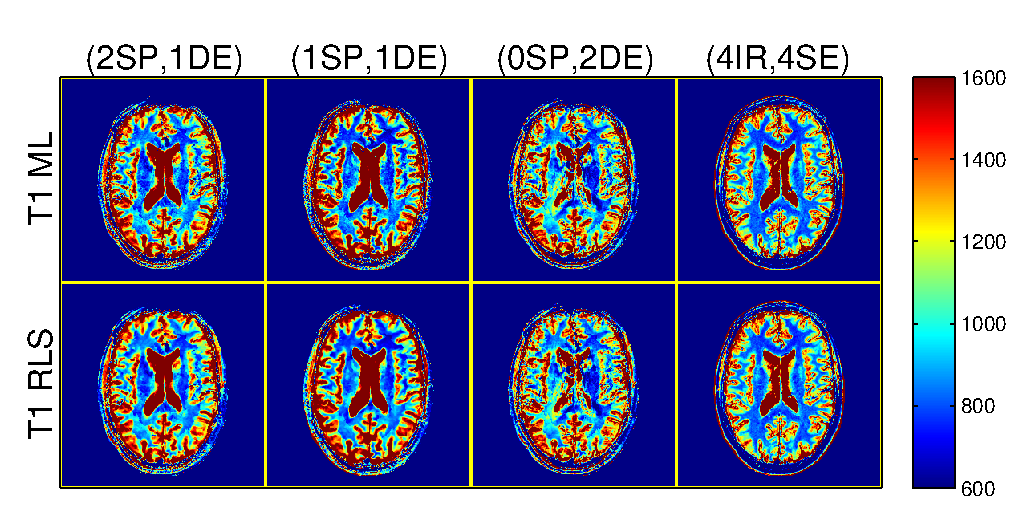
\includegraphics [width=15.4cm] {2016-05-31,brain,t1,jet.eps}
		\label{fig:brain,t1,jet}
	}
	\vspace{0cm}
	\subfigure{
		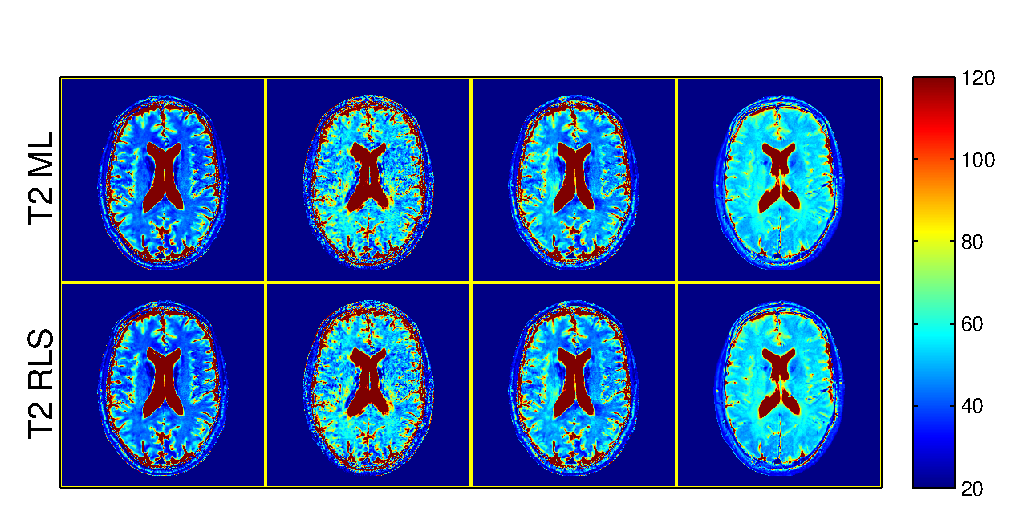
\includegraphics [width=15.2cm, trim=0 0 0 25, clip] {2016-05-31,brain,t2,jet.eps}
		\label{fig:brain,t2,jet}
	}
	\caption{
		Colorized $\bmTo$ and $\bmTt$ ML and RL estimates 
		from the brain of a healthy volunteer.
		Columns correspond to profiles consisting 
		of (2~SPGR,~1~DESS), (1~SPGR,~1~DESS), (0~SPGR,~2~DESS), 
		and (4~IR,~4~SE) acquisitions.  
		Rows distinguish $\bmTo$ and $\bmTt$ ML and RL estimators.
		Table~\ref{table:brain} presents corresponding WM/GM 
		within-ROI sample statistics.
		Colorbar ranges are in milliseconds.
	}
	\label{fig:brain,jet}
\end{figure*}

Fig.~\ref{fig:brain,jet} compares 
brain $\bmTo$ and $\bmTt$ ML and RL estimates 
from optimized scan profiles.
Though in-plane motion is largely compensated via registration, 
through-plane motion and non-bulk motion likely persist, 
and will influence ROI statistics.
Due to motion (and scan duration) considerations,
we examine within-ROI statistics from a single repetition 
as in Section~\ref{sss,scn-dsgn,exp,phant,roi}, 
and do not attempt across-repetition statistics 
as in Section~\ref{sss,scn-dsgn,exp,phant,rep}.
	
Visually, $\bmToest$ maps from steady-state profiles 
exhibit similar levels of contrast 
in WM/GM regions well away 
from cerebrospinal fluid (CSF) as that seen 
in the reference $\bmToest$ estimate.
Since we did not optimize any scan profiles 
for estimation in high-$\To$ regions, 
it is expected that greater differences may emerge 
in voxels containing or nearby CSF. 
In particular, 
$\bmTo$ is significantly underestimated 
within and near CSF by the $(0,2)$ DESS-only profile. 
This suggests that with the signal models used in this work, 
including at least one SPGR scan in an optimized profile 
may offer greater protection 
against estimation bias in high-$\To$ regions.

% t1/t2 ml brain summary table
\begin{table*} [tb]
	\centering
	\small
	\begin{minipage}{0.18\textwidth}
		\includegraphics [width=2.8cm] {2016-05-31,brain,roi,gray.eps}
		\label{fig:brain,roi,gray}
	\end{minipage}
	\begin{minipage}{0.8\textwidth}
		\begin{tabu} {c | c | r r r | r}
			\hline \hline
				& ROI			& (2SP,1DE)				& (1SP,1DE) 			& (0SP,2DE)				& (4IR,4SE) \\
			\hline
			\multirow{5}{*}{$\ToML$} 	
			& \AR WM	& $840 \pm 32$		& $770 \pm 31$ 		& $840 \pm 43$ 		& $780 \pm 22$ \\
			& \AL WM 	& $740 \pm 61$ 		& $660 \pm 45$ 		& $740 \pm 55$ 		& $760 \pm 24$ \\
			& \PR WM 	& $890 \pm 88$ 		& $860 \pm 72$ 		& $960 \pm 84$ 		& $810 \pm 26$ \\
			& \PL WM 	& $860 \pm 70.$ 	& $850 \pm 61$ 		& $880 \pm 79$ 		& $820 \pm 37$ \\
			& \A GM 	& $1200 \pm 210$	& $1200 \pm 230$ 	& $1300 \pm 230$	& $1300 \pm 180$ \\
			\hline
			\multirow{5}{*}{$\ToRL$} 	
			& \AR WM	& $840 \pm 24$		& $770 \pm 20.$		& $840 \pm 43$ 		& $780 \pm 20.$ \\
			& \AL WM 	& $740 \pm 51$ 		& $670 \pm 37$ 		& $740 \pm 54$ 		& $760 \pm 23$ \\
			& \PR WM 	& $890 \pm 79$ 		& $860 \pm 61$ 		& $960 \pm 82$ 		& $810 \pm 24$ \\
			& \PL WM 	& $870 \pm 62$ 		& $850 \pm 50.$		& $880 \pm 78$ 		& $820 \pm 35$ \\
			& \A GM 	& $1200 \pm 200$	& $1200 \pm 220$ 	& $1300 \pm 230$	& $1300 \pm 180$ \\
			\hline \hline
			\multirow{5}{*}{$\TtML$} 	
			& \AR WM 	& $40. \pm 1.3$ 	& $54 \pm 3.8$ 		& $46 \pm 1.5$		& $55 \pm 1.9$ \\
			& \AL WM 	& $40. \pm 1.7$		& $50. \pm 4.5$		& $44 \pm 1.7$ 		& $53 \pm 1.8$ \\
			& \PR WM  & $43 \pm 2.7$ 		& $60. \pm 6.9$ 	& $51 \pm 3.6$ 		& $59 \pm 2.1$ \\
			& \PL WM 	& $43 \pm 1.8$		& $57 \pm 4.9$ 		& $49 \pm 2.5$ 		& $57 \pm 1.8$ \\
			& \A GM 	& $50 \pm 12$ 		& $60 \pm 15$ 		& $60 \pm 11$ 		& $59 \pm 6.0$ \\
			\hline
			\multirow{5}{*}{$\TtRL$} 	
			& \AR WM  & $40. \pm 1.3$ 	& $54 \pm 3.4$ 		& $46 \pm 1.5$		& $55 \pm 1.9$ \\
			& \AL WM 	& $40. \pm 1.7$		& $50. \pm 4.4$		& $43 \pm 1.7$ 		& $53 \pm 1.8$ \\
			& \PR WM  & $43 \pm 2.8$ 		& $60. \pm 6.7$ 	& $51 \pm 3.7$ 		& $58 \pm 2.3$ \\
			& \PL WM 	& $43 \pm 1.7$		& $57 \pm 4.7$ 		& $49 \pm 2.5$ 		& $57 \pm 1.8$ \\
			& \A GM 	& $50 \pm 12$ 		& $60 \pm 15$ 		& $60 \pm 11$ 		& $59 \pm 6.4$ \\
			\hline \hline
		\end{tabu}
	\end{minipage}
	\vspace{1mm}
	\caption{
		\emph{Left}:
		WM/GM ROIs,
		overlaid on a representative anatomical
		(coil-combined, IR) image.
		Separate WM ROIs are distinguished
		by anterior-right (\AR),
		anterior-left (\AL),
		posterior-right (\PR), and
		posterior-left (\PL) directions.
		Four small anterior (\A) cortical GM polygons
		are pooled into a single ROI.
		\emph{Right}:
		Within-ROI sample means $\pm$ 
		within-ROI sample standard deviations 
		of $\bmTo$ and $\bmTt$ ML and RL estimates 
		from the brain of a healthy volunteer
		(Fig.~\ref{fig:brain,jet} presents corresponding images).
		Sample statistics are computed 
		within ROIs indicated in the anatomical image.  
		All values are reported in milliseconds.
	}
	\label{table:brain}
\end{table*} 

Table~\ref{table:brain} summarizes 
within-ROI sample means and sample standard deviations 
computed\footnote{We have taken effort 
to select ROIs that reflect expected anatomy 
in all coil-combined and registered images, 
including adjacent slices in images from 3D acquisitions. 
However, we acknowledge the possibility 
of some contamination across tissue boundaries, 
especially WM and/or CSF contamination into cortical GM.
}
over four separate WM ROIs containing 96, 69, 224, and 148 voxels 
and one pooled cortical GM ROI containing 156 voxels.	
Within-ROI $\bmToest$ sample standard deviations are comparable 
across SS profiles.
In agreement with Table~\ref{table:profile}, 
$\bmTt$ estimates from the optimized $(1,1)$ scan profile 
exhibit higher within-ROI sample variation 
than corresponding $(2,1)$ and $(0,2)$ $\bmTtest$ maps.
Compared to ML counterparts,
RL estimates generally reduce within-ROI sample variation
and do not significantly change within-ROI sample means.

In most cases, $\bmToest$ within-ROI sample means 
from optimized SPGR/DESS scan profiles 
do not deviate substantially from each other 
or from reference IR/SE measurements.
Two notable exceptions are $\ToML$ 
in anterior left and posterior right WM 
from $(1,1)$ and $(0,2)$ profiles: 
these estimates are significantly lower and higher 
than analogous estimates from other profiles, respectively.
Results thus suggest that the optimized $(2,1)$ scan profile 
yields WM $\ToML$ estimates 
that are more consistently similar to IR WM $\ToML$ estimates 
than other optimized SPGR/DESS profiles.

Systematic differences in $\bmTtest$ sample means 
are evident across scan profiles, 
particularly within WM ROIs.
Curiously, the $(1,1)$ profile agrees most consistently 
(in WM/GM $\TtML$ within-ROI sample mean) 
with reference estimates, 
though with relatively high sample variation.
The $(2,1)$ and $(0,2)$ SPGR/DESS profiles 
produce consistently lower WM $\TtML$ 
than the reference IR/SE profile, 
though the $(0,2)$ profile is in reasonable agreement 
with other steady-state estimates \cite{heule:14:tes-nib}.
These discrepancies may due to differences 
in sensitivity to multi-compartmental relaxation \cite{mackay:94:ivv}.
Specifically, different signal models 
with different scan parameter choices 
might be more or less sensitive 
to the model mismatch incurred 
by neglecting to distinguish 
the multiple $\Tt$ components within each voxel.
Chapter~\ref{c,mwf} studies multi-compartmental relaxation 
in much greater detail.

%%%%%%%%%%%%%%%%%%%%%%%%%%%%%%%%%%%%%%%%%%%%%%%%%%%
\section{Discussion and Future Work}
\label{s,scn-dsgn,disc}
%%%%%%%%%%%%%%%%%%%%%%%%%%%%%%%%%%%%%%%%%%%%%%%%%%%

Phantom experiments show 
that optimized scan profiles consisting 
of $(2,1)$, $(1,1)$, and $(0,2)$ (SPGR, DESS) scans 
yield accurate WM/GM $\To,\Tt$ estimates, 
and that empirical precision trends across profiles agree reasonably 
with CRB-based predictions.
However, \emph{in vivo} experiments reveal 
that even with scan optimization, 
it may be challenging to achieve clinically viable levels 
of precision from the aforementioned SS profiles, at least at 3T. 
At the expense of greater scan time, 
it is of course possible that optimized profiles 
containing greater numbers of SPGR, DESS, and/or other SS scans 
can provide clinically acceptable precision levels.
For these and other more complicated scan profiles, 
estimator dependence on scan parameters becomes even less intuitive, 
increasing the need for scan design.

The proposed scan design framework addresses spatial variation 
in object parameters through a min-max design criterion.
The min-max criterion guarantees an upper bound 
on a weighted sum of variances 
and assumes no prior knowledge of distributions.
However, in general it is non-differentiable 
in $\bmP$, precluding gradient-based optimization. 	
Furthermore, it is conservative by nature, 
and often selects scan parameters based 
on corner cases of the object parameter space.
To reduce the influence of corner cases, 
it may be desirable to instead construct a cost function 
related to the coefficient of variation 
as in \cite{jones:96:oss, zhang:98:dos, imran:99:tpm, deoni:04:doo}, 
perhaps by setting parameter weights $\bmW^{-1} \gets \diag{\bmx}$ 
for $\bmx \neq 0$ in \eqref{eq:scn-dsgn,cost}.
	
As a less conservative alternative 
to min-max design, 
other recent works \cite{akcakaya:15:ots, lewis:16:ddo} 
have addressed object parameter spatial variation 
by instead constructing cost functions related 
to the Bayesian CRB \cite{gill:95:aot}, 
which characterizes the expected precision 
with respect to a prior distribution on object parameters.
Bayesian cost functions are usually differentiable and can also, 
with appropriate priors, 
penalize object parameter coefficients of variation 
instead of variances, 
as in \cite{akcakaya:15:ots}.
However, prior distributions are generally unknown, 
and may need to be estimated from data, 
as in \cite{lewis:16:ddo}.

Careful calibration of flip angle scaling $\bmstx$ is essential 
for accurate $\bmTo, \bmTt$ estimation 
from SPGR/DESS scan profiles. 
In this work, we estimate $\bmstx$ 
from \emph{separate} acquisitions 
and adjust nominal flip angles prior to reconstruction, 
but acknowledge that non-idealities 
in those separate acquisitions may themselves 
cause resultant transmit field estimation errors 
to propagate into our $\bmTo,\bmTt$ estimates. 
To reduce error propagation, 
it may be desirable to instead design scan profiles 
to permit \emph{joint} estimation of $\bmstx$, 
in addition to other latent object parameters.
Unfortunately, 
we find that optimizing the $(2,1)$ or $(0,2)$ profile 
to allow for four-parameter 
$\bmx\pr \gets \brac{\To\pr, \Tt\pr, \const{2}\pr, \stx\pr}\tpose$ estimation 
results in unacceptably high amplification 
of the worst-case $\To$ standard deviation. 
(Incidentally however, precise $\bmTt$ ML and RL estimation alone 
from the $(2,1)$ or $(0,2)$ profile 
is possible \cite{nataraj:14:mbe}.) 
It remains an open scan design question 
as to whether time spent collecting Bloch-Siegert data 
for separate $\bmstx$ mapping could instead be better spent 
collecting additional SPGR, DESS, 
and/or other data for joint estimation.

By working with closed-form signal expressions, 
we neglect to model several higher-order effects.
However, it is apparent 
that the nonlinear estimation procedures required 
for many mapping problems can amplify the influence 
of these secondary effects, 
often inducing substantial bias. 
Since the CRB (as described) 
applies only to unbiased estimators, 
it is thus desirable to use signal models 
that are as complete as possible 
for CRB-based scan design.
In theory, scan optimization approach \eqref{eq:scn-dsgn,P-star} 
is even compatible with acquisitions 
where a closed-form model relating data 
to latent and scan parameters is unknown, 
as in \cite{beneliezer:15:raa, ma:13:mrf}. 
In practice, difficulties arise in efficient computation 
of signal gradients required in \eqref{eq:scn-dsgn,fisher},
which may demand more specialized techniques, 
as in \cite{zhao:16:oed}.
Designing scan profiles involving such complex signal models 
would likely necessitate optimization techniques more involved 
than the simple grid searches used in this work.

%%%%%%%%%%%%%%%%%%%%%%%%%%%%%%%%%%%%%%%%%%%%%%%%%%%
\section{Conclusion}
\label{s,scn-dsgn,conc}
%%%%%%%%%%%%%%%%%%%%%%%%%%%%%%%%%%%%%%%%%%%%%%%%%%%

This chapter has introduced 
a CRB-inspired min-max optimization approach 
to guide MR scan design 
for precise parameter estimation. 
As a detailed example, 
we have optimized combinations 
of fast SPGR and DESS scans 
for $\To, \Tt$ relaxometry 
in WM and GM regions of the human brain at 3T. 
Numerical simulations show that at typical noise levels 
and with accurate flip angle prior knowledge, 
WM- and GM-like $\To, \Tt$ ML estimates 
from optimized scans are nearly unbiased,
and so worst-case CRB predictions 
yield reliable bounds on ROI sample variances.
Phantom accuracy experiments show that optimized combinations 
of $(2,1)$, $(1,1)$, or $(0,2)$ (SPGR, DESS) scans 
are in excellent agreement with NIST and IR/SE measurements 
over the designed latent object parameter range of interest.
Phantom precision experiments show 
that these SPGR/DESS combinations exhibit trends 
in pooled sample standard deviations 
that reasonably reflect CRB predictions.

\emph{In vivo} experiments suggest that with optimization, 
the $(0,2)$ profile can yield comparable $\bmToest, \bmTtest$ precision 
to the more conventional $(2,1)$ \cite{nataraj:14:mbe} scan profile 
in well-isolated WM/GM ROIs; 
however, the $(0,2)$ $\bmTo$ estimates are unreliable 
within and near the CSF
and do not agree with IR measurements 
in WM as consistently as the $(2,1)$ profile.
This and other disagreements across profiles \emph{in vivo} 
may be attributable to differences in signal model sensitivities 
to neglected higher-order effects. 
Nevertheless, the example application 
studied in this chapter illustrates 
that scan optimization can enable new parameter mapping techniques 
from established pulse sequences.


% \chapter{Dictionary-Free MRI Parameter Estimation via KRR}
% \label{c,krr}
% % kernel ridge regression for parameter estimation



\chapter{QMRI Parameter~Estimation via~Regression~with~Kernels (PERK)}
\label{c,perk}
% mri parameter estimation via regression with kernels (PERK)

%%%%%%%%%%%%%%%%%%%%%%%%%%%%%%%%%%%%%%%%%%%%%%%%%%%
\section{Introduction}
\label{s,perk,intro}
%%%%%%%%%%%%%%%%%%%%%%%%%%%%%%%%%%%%%%%%%%%%%%%%%%%

In quantitative magnetic resonance imaging (QMRI),
one seeks to estimate latent parameter images 
from suitably informative data.
Since MR acquisitions are tunably sensitive 
to many physical processes
(\eg, relaxation \cite{bloch:1946:ni-paper}, 
diffusion \cite{torrey:56:bew},
and chemical exchange \cite{mcconnell:58:rrb}),
MRI parameter estimation is important
for many QMRI applications
(\eg, relaxometry \cite{bloembergen:1948:rei}, 
diffusion tensor imaging \cite{bihan:01:dti}, 
and multi-compartmental imaging \cite{mackay:94:ivv}). 
Motivated by widespread applications,
this chapter introduces a general method
for fast MRI parameter estimation.

% signal models nonlinear
% so parameter estimation requires nonconvex optimization
% previous chapter described likelihood models
% several works [cite] have had success with this
% however these work for simple problems like single t1/t2 estimation
% for larger problems, undesirable or even intractable
% staroswiecki:12:seo 	fit m0,t1,t2,adc from dess im per-voxel
% ma:13:mrf		 					fit m0,t1,t2,b0 from mrf im per-voxel
% mcgivney:14:scf 	 		fit m0,t1,t2,b0 from low-rank mrf im using low-rank dict per-voxel
% zhao:14:mbm						recon m0,t2 from sse data via sparsity-constrained recon
% zhao:15:amp 					low-rank plus sparse recon w varpro for t1,t2 mapping
% beneliezer:15:raa 		fit m0,t2,b1 from mse im per-voxel
% zhao:16:mlr						recon m0,t1,t2 maps from mrf data via admm/varpro
% nataraj:17:oms				fit m0,t1,t2 from spgr/dess per-voxel
% asslander::lra 				similar to zhao:16:mlr, but claims better-conditioned initialization?
% cauley:15:fgm 				cluster full dict elements; use dict means to fit m0,t1,t2,b0 per-voxel
% doneva:17:mcb					est subspace of mrf k-t data from fully-sampled k-space center
% 											use subspace est for low-rank matrix completion of mrf data
% 											then recon matrix-completed mrf data and fit m0,t1,t2 per-voxel
% yang::lra 						fit m0,t1,t2,b0 from low-rank mrf im using coarse low-rank dict per-voxel
%												and then apply bilinear interpolation: x100 acceleration
Chapter~\ref{c,relax} applied
a common parameter estimation strategy to QMRI
that involves minimizing a cost function
related to a statistical likelihood function.
Because MR signal models are typically nonlinear functions
of the underlying latent parameters,
such likelihood-based estimation
usually requires non-convex optimization.
To seek good solutions,
many works
(\eg, 
\cite{%
	haldar:07:mle,%
	hernando:08:jeo,%
	barral:10:arm,%
	staroswiecki:12:seo,%
	ma:13:mrf,%
	trzasko:13:etf,%
	mcgivney:14:scf,%
	zhao:14:mbm,%
	beneliezer:15:raa,%
		zhao:15:amp,%
	cauley:15:fgm,%
	zhao:16:mlr,%
	nataraj:17:oms,%
	asslander::lra,%
	yang::lra%
})
approach estimation
with algorithms
that employ exhaustive grid search,
which requires either storing
or computing on-the-fly 
a ``dictionary'' of signal vectors.
These works estimate a small number (2-3)
of nonlinear latent parameters,
so grid search is practical.
However, 
for moderate or large sized problems,
the required number 
of dictionary elements
renders grid search undesirable or even intractable,
unless one imposes artificially restrictive latent parameter constraints.
Though several recent works
\cite{%
	mcgivney:14:scf,%
	cauley:15:fgm,%
	asslander::lra,%
	yang::lra%
}
focus on reducing dictionary storage requirements,
all of these methods ultimately rely 
on some form of dictionary-based grid search.

% clear need for a method that scales well with # parameters?
% multi-compartment: 6-11
% diffusion: at least 7
% phase-based methods: flow, b1, b0, asl? 
There are numerous QMRI applications
that could benefit from an alternative parameter estimation method
that scales well with the number of latent parameters.
For example,
vector (\eg, flow \cite{feinberg:85:mri})
and tensor 
(\eg, diffusivity \cite{bihan:01:dti} or conductivity \cite{tuch:01:ctm})
field mapping techniques
require estimation 
of at minimum 4 and 7 latent parameters per voxel,
respectively.
Phase-based longitudinal \cite{sekihara:85:nif} 
or transverse \cite{morrell:08:aps,sacolick:10:bmb} field mapping
could avoid noise-amplifying algebraic manipulations
on reconstructed image data
that are conventionally used
to reduce signal dependencies 
on nuisance latent parameters.
Compartmental fraction mapping \cite{mackay:94:ivv,nataraj:17:mwf}
from steady-state pulse sequences
requires estimation of at least 7 \cite{deoni:08:gmt}
and as many as 10 \cite{deoni:13:oct}
latent parameters per voxel.
In these and other applications,
greater estimation accuracy
requires more complete signal models
that involve more latent parameters,
increasing the need 
for scalable estimation methods.

% kernel methods
% fundamental challenge: nonlinear model
% classical idea: transform nonlinear problem into a linear one
% unclear how to balance complexity of transformation for accuracy with increase in dimensionality
% fortunately, simple transforms involving certain reproducing kernel functions yield solutions that need not scale in complexity with the dimensionality of the associated transformed data
% wahba introduced representation in approx theory
% scholkopf introduced in context of learning theory
% enjoyed success in many machine learning applications,
% originally for classification and later regression
The fundamental challenge 
of scalable MRI parameter estimation
stems from MR signal model nonlinearity:
standard linear estimators
would be scalable but inaccurate.
One natural solution strategy
involves nonlinearly preprocessing reconstructed images
such that the transformed images 
are at least approximately linear
in the latent parameters.
As an example,
for simple $\Tt$ estimation
from measurements at multiple echo times,
one could apply linear regression
to the logarithm of the measurements
(Section~\ref{s,demo} builds further intuition
using this simple application).
However,
such simple transformations
are generally not evident 
for more complicated signal models.
Without such problem-specific insight,
sufficiently rich nonlinear transformations
could dramatically increase problem dimensionality,
hindering scalability.
Fortunately, 
a celebrated result
in approximation theory \cite{kimeldorf:70:acb} showed
that simple transformations involving
\emph{reproducing kernel} functions \cite{aronszajn:50:tor}
can represent nonlinear estimators
whose evaluation need not directly scale in computation
with the (possibly very high) dimension
of the associated transformed data.
These kernel methods later found popularity
in machine learning
(initially for classification \cite{cortes:95:svn}
and quickly thereafter for other applications,
\eg, regression \cite{saunders:98:rrl})
because they provided simple, scalable nonlinear extensions
to fast linear algorithms.

% related work
The general idea
of using linearization
to simplify a nonlinear estimation problem
has been used before in QMRI.
For example,
orthogonal transforms
have been used
to linearly represent 
exponential \cite{huang:12:tmf}
and extended phase graph \cite{huang:13:trw} models
for $\Tt$ estimation.
An unscented Kalman filter 
has been used 
to linearly represent nonlinear models
for general multiple-parameter estimation
up to third-order accuracy \cite{zhao:16:daa}.
Whereas these prior works largely focus
on parameter estimation accuracy gains 
in under-sampled acquisitions,
this paper focuses on acceleration 
for general per-voxel MRI parameter estimation
from reconstructed images.

% idea here is to link parameter estimation 
% to a problem of regression
% ideas of machine learning can link estimation (seek parameter estimates from data assuming model) to regression (seek regression function relating inputs to outputs)
This chapter introduces  
a fast dictionary-free method
for MRI parameter estimation
via regression with kernels (PERK).
PERK first simulates many instances
of latent parameter inputs
and measurement outputs
using prior distributions
and a general nonlinear MR signal model.
PERK takes such input-output pairs
as simulated \emph{training points}
and then \emph{learns}
(using an appropriate nonlinear kernel function)
a nonlinear \emph{regression function}
from the training points.
PERK may scale considerably better
with the number of latent parameters
than likelihood-based estimation 
via grid search.

The remainder of this chapter
is organized as follows.
Section~\ref{s,perk,rev} reviews 
pertinent background information about kernels. 
Section~\ref{s,perk,meth} formulates 
a function optimization problem
for MRI parameter estimation
and efficiently solves this problem 
using kernels.
Section~\ref{s,perk,perf} studies bias and covariance
of the resulting PERK estimator.
Section~\ref{s,perk,pract} addresses practical implementation issues
such as computational complexity and model selection.
Section~\ref{s,perk,exp} demonstrates PERK
in numerical simulations
as well as phantom and \invivo experiments.
Section~\ref{s,perk,disc} discusses advantages,
challenges, and extensions.
Section~\ref{s,perk,conc} summarizes key contributions.

%%%%%%%%%%%%%%%%%%%%%%%%%%%%%%%%%%%%%%%%%%%%%%%%%%%
\section{Preliminaries}
\label{s,perk,rev}
%%%%%%%%%%%%%%%%%%%%%%%%%%%%%%%%%%%%%%%%%%%%%%%%%%%

This brief section reviews
relevant definitions and facts about kernels.
A (real-valued) \emph{kernel} 
$k : \setQ^2 \mapsto \real$
is a function 
that describes a measure of similarity
between two pattern vectors 
$\bmq,\bmq' \in \setQ$.
The matrix $\bmK \in \reals{N \times N}$
associated with kernel $k$
and $N \in \setN$ patterns $\bmq_1,\dots,\bmq_N \in \setQ$
consists of entries
$k\paren{\bmq_n,\bmq_{n'}}$
for $n,n' \in \set{1,\dots,N}$.
A \emph{positive definite kernel} is a kernel
for which $\bmK$ is positive semidefinite (PSD)
for any finite set of pattern vectors,
in which case $\bmK$
is a \emph{Gram matrix}.
A \emph{symmetric kernel} satisfies 
$k\paren{\bmq,\bmq'} = k\paren{\bmq',\bmq}$
$\forall \bmq,\bmq' \in \setQ$.
We hereafter restrict attention
to symmetric, positive definite (SPD) kernels.

An SPD kernel $k : \setQ^2 \mapsto \real$
defines an inner product 
in a particular Hilbert function space $\rkhs$
that we briefly describe here
because it characterizes
the class of candidate regression functions
over which PERK operates.
To envision $\rkhs$,
first define a kernel's associated \emph{(canonical) feature map} 
$\bmz : \setQ \mapsto \reals{\setQ}$
that assigns each $\bmq \in \setQ$ 
to a \emph{(canonical) feature} $k\paren{\cdot,\bmq} \in \reals{\setQ}$.
Then $\rkhs$ is a completion 
of the space $\setH := \set{\sum_{n=1}^N a_n k\paren{\cdot,\bmq_n}}$
spanned by point evaluations
of the feature map,
where
$N \in \setN$,
$a_1,\dots,a_N \in \real$,
and
$\bmq_1,\dots,\bmq_N \in \setQ$ are arbitrary.
Let $\innprod{\cdot}{\cdot} : \rkhs^2 \mapsto \real$ 
denote the inner product on $\rkhs$.
Then for any $h,h' \in \setH$
that have finite-dimensional canonical representations
$h := \sum_{n=1}^N a_n k\paren{\cdot,\bmq_n}$ 
and
$h' := \sum_{n'=1}^N b_{n'} k\paren{\cdot,\bmq_{n'}}$,
the assignment
\begin{align}
	\innprod{h}{h'}_\rkhs =
		\sum_{n=1}^N \sum_{n'=1}^N a_n b_{n'} k\paren{\bmq_{n'},\bmq_n}
	\label{eq,inn-prod}
\end{align}
is consistent
with the inner product on $\rkhs$.
This inner product exhibits $\forall h\in\rkhs, \bmq\in\setQ$
an interesting \emph{reproducing property}
\begin{align}
	\innprod{h}{k\paren{\cdot,\bmq}}_\rkhs = h\paren{\bmq}
	\label{eq,rep-prop}
\end{align}
that can be seen to directly follow 
from \eqref{eq,inn-prod}
for $h \in \setH$.

A \emph{reproducing kernel} (RK) is a kernel 
that satisfies \eqref{eq,rep-prop}
for some real-valued Hilbert space $\rkhs$.
A kernel is reproducing if and only if it is SPD.
There is a bijection between RK $k$ and $\rkhs$,
and so $\rkhs$ is often called
the \emph{reproducing kernel Hilbert space} (RKHS)
uniquely associated with RK $k$.
This bijection is critical
to practical function optimization over an RKHS
in that it translates inner products 
in a (usually high-dimensional) RKHS $\rkhs$
into equivalent kernel operations 
in the (lower-dimensional) pattern vector space $\setQ$.
The following sections exploit 
the bijection between an RKHS 
and its associated RK.

%%%%%%%%%%%%%%%%%%%%%%%%%%%%%%%%%%%%%%%%%%%%%%%%%%%
\section{A Function Optimization Problem \& Kernel Solution}
\label{s,perk,meth}
%%%%%%%%%%%%%%%%%%%%%%%%%%%%%%%%%%%%%%%%%%%%%%%%%%%

After image reconstruction,
many QMRI acquisitions 
produce at each voxel position
a sequence of noisy measurements
$\bmy \in \complexes{D}$, 
modeled as
\begin{align}
	\bmy = \bmsa{\bmx, \bmnu} + \bmeps,
	\label{eq,model}
\end{align}
where $\bmx \in \reals{L}$ denotes $L$ \emph{latent} parameters;
$\bmnu \in \reals{K}$ denotes $K$ \emph{known} parameters;  
$\bms : \reals{L} \times \reals{K} \mapsto \complexes{D}$ 
models $D$ noiseless continuous signal functions;
and $\bmeps \sim \cgauss{\zeros{D}}{\bmSig}$ is complex Gaussian noise
with zero mean $\zeros{D} \in \reals{D}$
and known covariance $\bmSig \in \reals{D \times D}$.
(As a concrete example,
for $\Tt$ estimation
from single spin echo measurements,
$\bmx$ could collect spin density and $\Tt$;
$\bmnu$ could collect known longitudinal and transverse field inhomogeneities;
and 
$\bmy$ could collect measurements at $D$ echo times.)
We seek to estimate 
on a per-voxel basis
each latent parameter $\bmx$
from measurement $\bmy$ 
and known parameter $\bmnu$.

To develop an estimator $\est{\bmx}$,
we simulate many instances 
of forward model \eqref{eq,model}
and use kernels
to estimate a nonlinear inverse function.
We sample part of $\reals{L} \times \reals{K} \times \complexes{D}$
and evaluate \eqref{eq,model} $N$ times
to produce sets of object parameter and noise realizations
$\set{\paren{\bmx_1,\bmnu_1,\bmeps_1},\dots,\paren{\bmx_N,\bmnu_N,\bmeps_N}}$
and corresponding measurements
$\set{\bmy_1,\dots,\bmy_N}$. 
We seek a function
$\est{\bmh}~:~\reals{\dimQ} \mapsto \reals{L}$
and an offset $\est{\bmb} \in \reals{L}$
that together map each pure-real
\footnote{%
	We present our methodology 
	assuming pure-real patterns $\bmq$ 
	and estimators $\est{\bmx}$
	for simplicity and 
	to maintain consistency
	with experiments,
	in which we choose to use magnitude images
	for unrelated reasons 
	(see \S\ref{ss,exp,meth} for details). 
	It is straightforward 
	to generalize Theorem~\ref{thm,rep}
	for complex-valued kernels 
	and thereby address the cases 
	of complex patterns and/or estimators.
}
regressor $\bmq_n := [\abs{\bmy_n}\tpose, \bmnu_n\tpose]\tpose$
to an estimate 
$\bmxha{\bmq_n} := \bmhha{\bmq_n}+\est{\bmb}$ 
that is ``close'' 
to corresponding regressand $\bmx_n$,
where $\dimQ := D+K$,
$n \in \set{1,\dots,N}$,
and $\paren{\cdot}\tpose$ denotes vector transpose.
For any finite $N$,
there are infinitely many candidate estimators
that are consistent with training points
in this manner.
We use function regularization
to choose one estimator
that smoothly interpolates 
between training points:
\begin{align}
	\paren{\est{\bmh},\est{\bmb}} &\in 
		\argmin{\substack{\bmh \in \rkhs^L \\ \bmb \in \reals{L}}}
		\costa{\bmh, \bmb; \set{\paren{\bmx_n,\bmq_n}}_{1}^N}, 
		\where \label{eq,prob} \\
	\costa{\dots} &= 
		\sum_{l=1}^L \cost_l\paren{h_l,b_l; \set{\paren{x_{l,n},\bmq_n}}_{1}^N}; 
		\label{eq,cost} \\
	\Psi_l(\dots) &= 
		\rho_l \norm{h_l}_\rkhs^2 + 
		\frac{1}{N} \sum_{n=1}^N \paren{h_l(\bmq_n) + b_l - x_{l,n}}^2.
		\label{eq,cost-l}
\end{align}
Here, each $h_l~:~\reals{\dimQ} \mapsto \real$ is a scalar function
that maps to the $l$th component of the output of $\bmh$; 
each $b_l,x_{l,n} \in \real$ are scalar components of $\bmb,\bmx_n$;
$\rkhs$ is an RKHS 
whose norm $\norm{\cdot}_\rkhs$ 
is induced by inner product 
$\innprod{\cdot}{\cdot}_\rkhs : \rkhs^2 \mapsto \real$; 
and each $\rho_l$ controls for regularity in $h_l$.

Since \eqref{eq,cost} is separable 
in the components of $\bmh$ and $\bmb$, 
it suffices to consider optimizing each $\paren{h_l,b_l}$ 
by separately minimizing \eqref{eq,cost-l} 
for each $l \in \set{1,\dots,L}$.
Remarkably,
a generalization of the Representer Theorem \cite{scholkopf:01:agr},
restated as is relevant here for completeness,
reduces minimizing \eqref{eq,cost-l} 
to a finite-dimensional optimization problem.
\begin{thm}[Generalized Representer, \cite{scholkopf:01:agr}]
	Define $k : \reals{Q} \times \reals{Q} \mapsto \real$
	to be the SPD kernel 
	associated with RKHS $\rkhs$, 
	such that reproducing property $h_l(\bmq) = \innprod{h_l}{k(\cdot,\bmq)}_\rkhs$
	holds for all $h_l \in \rkhs$ and $\bmq \in \reals{Q}$. 
	Then any minimizer $(\est{h}_l,\est{b}_l)$ of \eqref{eq,cost-l}
	over $\rkhs \times \real$
	admits a representation for $\est{h}_l$ of the form
	\label{thm,rep}
	\begin{align}
		\est{h}_l(\cdot) \equiv \sum_{n=1}^N a_{l,n} k(\cdot,\bmq_{n}),
		\label{eq,rep}
	\end{align}
	where each $a_{l,n} \in \real$ for $n \in \set{1,\dots,N}$.
\end{thm}

Thm.~\ref{thm,rep} ensures 
that any solution
to the component-wise 
$\paren{N+1}$-dimensional problem
\begin{align}
	(\est{\bma}_l,\est{b}_l) \in 
	&\argmin{\substack{\bma_l \in \reals{N} \\ b_l \in \real}} 
	\rho_l \norm{\sum_{n'=1}^N a_{l,n'} k(\cdot,\bmq_{n'})}^2_\rkhs + \nonumber \\
	&\frac{1}{N} \sum_{n=1}^N \paren{\sum_{n'=1}^N a_{l,n'} k(\bmq_n,\bmq_{n'}) + b_l - x_{l,n}}^2
	\label{eq,cvx}
\end{align}
corresponds via \eqref{eq,rep} 
to a minimizer of \eqref{eq,cost-l}
over $\rkhs \times \real$,
where $\bma_l := [a_{l,1},\dots,a_{l,N}]\tpose$.
Fortunately, a solution of \eqref{eq,cvx} exists uniquely
for $\rho_l > 0$
and can be expressed as
\begin{align}
	\est{\bma}_l &= \inv{\paren{\bmM \bmK \bmM + N\rho_l\eye{N}}} \bmM \bmxtl{l};
	\label{eq,a-hat} \\
	\est{b}_l &= \frac{1}{N} \ones{N}\tpose \paren{\bmxtl{l} - \bmK \est{\bma}_l},
	\label{eq,b-hat}
\end{align}
where 
$\bmK \in \reals{N \times N}$ is the Gram matrix 
consisting of entries $k(\bmq_n,\bmq_{n'})$ for $n,n' \in \set{1,\dots,N}$;
$\bmM := \eye{N}-\frac{1}{N}\ones{N}\ones{N}\tpose \in \reals{N \times N}$
is a de-meaning operator;
$\bmxtl{l} := [x_{l,1},\dots,x_{l,N}]\tpose$;
$\eye{N} \in \reals{N \times N}$ is the identity matrix;
and $\ones{N} \in \reals{N}$ is a vector of ones.
Substituting \eqref{eq,a-hat} into \eqref{eq,rep} 
yields an expression 
for the $l$th entry $\est{x}_l$ 
of MRI parameter estimator $\est{\bmx}$:
\begin{align}
	\est{x}_l\paren{\cdot} &\gets \bmxtl{l}\tpose 
		\paren{\frac{1}{N}\ones{N} + 
		\bmM\inv{\paren{\bmM\bmK\bmM + N\rho_l\eye{N}}} \bmka{\cdot}},
		\label{eq,xl-hat}
\end{align}
where
$\bmka{\cdot} := 
	\brac{k(\cdot,\bmq_1),\dots,k(\cdot,\bmq_N)}\tpose - \frac{1}{N}\bmK\ones{N}
	: \reals{Q} \mapsto \reals{N}$
is an embedding operator.

% utility of estimate depends on kernel function
% valid kernel is q'*q, which corresponds to linear ridge regression
% more useful kernel is nonlinear fun of q; we use gaussian
When $\rho_l>0\,\, \forall l \in \set{1,\dots,L}$, 
estimator $\bmxha{\cdot}$
with entries \eqref{eq,xl-hat} minimizes \eqref{eq,cost}
over $\rkhs^L \times \real^L$.
However, the utility of $\bmxha{\cdot}$
depends on the choice of kernel $k$,
which induces a choice on the RKHS $\rkhs$
and thus the function space $\rkhs^L \times \real^L$
over which \eqref{eq,prob} optimizes.
For example, if $k$ was selected as the canonical dot product 
$k(\bmq,\bmq') \gets \innprod{\bmq}{\bmq'}_{\reals{Q}} := \bmq\tpose \bmq'$
(for which RKHS $\rkhs \gets \reals{Q}$),
then \eqref{eq,xl-hat} would reduce 
to affine ridge regression \cite{hoerl:70:rrb}
which is optimal over $\reals{Q} \times \real$
but is unlikely to be useful 
when signal model $\bms$ is nonlinear in $\bmx$.
Since we expect a useful estimate $\est{\bmx}\paren{\bmq}$ 
to depend nonlinearly (but smoothly) 
on $\bmq$ in general, 
we instead use 
an SPD kernel $k$ 
that is likewise nonlinear in its arguments
and thus corresponds to an RKHS much richer than $\reals{Q}$. 
Specifically, we use a Gaussian kernel
\begin{align}
	k(\bmq,\bmq') \gets \expa{-\frac{1}{2}{\norm{\bmq-\bmq'}^2_{\bmL^{-2}}}},
	\label{eq,kern}
\end{align}
where positive definite matrix bandwidth $\bmL \in \reals{Q \times Q}$ 
controls the length scales in $\bmq$ over which 
the estimator $\est{\bmx}$ smooths
and $\norm{\cdot}_{\bmG} \equiv \norm{\bmG^{1/2}\paren{\cdot}}_2$
is a weighted $\ell^2$-norm
with PSD matrix weights $\bmG$.
We use a Gaussian kernel
over other candidates
because it is a \emph{universal kernel},
meaning weighted sums of the form 
$\sum_{n=1}^N a_n k\paren{\cdot,\bmq_n}$
can approximate $\Ltwo$ functions
to arbitrary accuracy
for $N$ sufficiently large
\cite{steinwart:08:svm}.

Interestingly, 
the RKHS associated 
with Gaussian kernel \eqref{eq,kern}
is infinite-dimensional.
Thus, 
Gaussian kernel regression
can be interpreted as 
first ``lifting'' 
via a nonlinear \emph{feature map} 
$\bmz : \reals{Q} \mapsto \rkhs$ 
each $\bmq$ 
into an infinite-dimensional \emph{feature} 
$\bmza{\bmq} = k\paren{\cdot,\bmq} \in \rkhs$,
and then performing regularized affine regression
on the features
via dot products of the form
$\innprod{k\paren{\cdot,\bmq}}{k\paren{\cdot,\bmq'}}_{\rkhs}
	= k\paren{\bmq',\bmq}$.
From this perspective,
the challenges of nonlinear estimation 
via likelihood models
are avoided 
because we \emph{select} 
(through the choice of kernel) 
characteristics of the nonlinear dependence
that we wish to model
and need only \emph{estimate} via \eqref{eq,cvx} 
the linear dependence
of each entry in $\est{\bmx}$ 
on the corresponding features.

%%%%%%%%%%%%%%%%%%%%%%%%%%%%%%%%%%%%%%%%%%%%%%%%%%%
\section{Bias and Covariance Analysis}
\label{s,perk,perf}
%%%%%%%%%%%%%%%%%%%%%%%%%%%%%%%%%%%%%%%%%%%%%%%%%%%

%%%%%%%%%%%%%%%%%%%%%%%%%%%%%%%%%%%%%%%%%%%%%%%%%%%
\section{Implementation Considerations}
\label{s,perk,pract}
%%%%%%%%%%%%%%%%%%%%%%%%%%%%%%%%%%%%%%%%%%%%%%%%%%%

%%%%%%%%%%%%%%%%%%%%%%%%%%%%%%%%%%%%%%%%%%%%%%%%%%%
\section{Experimentation}
\label{s,perk,exp}
%%%%%%%%%%%%%%%%%%%%%%%%%%%%%%%%%%%%%%%%%%%%%%%%%%%

%%%%%%%%%%%%%%%%%%%%%%%%%%%%%%%%%%%%%%%%%%%%%%%%%%%
\section{Discussion}
\label{s,perk,disc}
%%%%%%%%%%%%%%%%%%%%%%%%%%%%%%%%%%%%%%%%%%%%%%%%%%%

%%%%%%%%%%%%%%%%%%%%%%%%%%%%%%%%%%%%%%%%%%%%%%%%%%%
\section{Conclusion}
\label{s,perk,conc}
%%%%%%%%%%%%%%%%%%%%%%%%%%%%%%%%%%%%%%%%%%%%%%%%%%%


% \chapter{Fast~Myelin~Water~Fraction~Imaging via~Acquisition~Design~and~PERK}
% \label{c,mwf}
% % myelin water fraction mapping

\todo{discuss negative $\ff$ range}



% \chapter{Future~Work}
% \label{c,future}
% % concluding remarks

This chapter suggests avenues
for further QMRI research,
focusing on relatively broad future directions
that this thesis has not explored.
Discussion sections
within main body chapters
offer more focused ideas 
for topic-specific extensions,
whereas the appendices organize 
partially investigated but still immature topics
that are less related to QMRI.

%%%%%%%%%%%%%%%%%%%%%%%%%%%%%%%%%%%%%%%%%%%%%%%%%%%
\section{%
	\edit{%
		Combining PERK with Image Reconstruction%
	}%
}%
\label{s,future,recon}
%%%%%%%%%%%%%%%%%%%%%%%%%%%%%%%%%%%%%%%%%%%%%%%%%%%

This thesis has considered parameter estimation
to be separate from image reconstruction.
This separation affords fast data processing
but may leave room for improved estimation performance,
especially when raw data is undersampled.
One could instead seek 
to estimate parameters 
directly from raw data.
One approach 
to combining image reconstruction
with PERK-based estimation
might seek to solve
the joint optimization problem
\begin{align}
	\paren{\est{\bmX},\est{\bmY}} &\in \set{%
		\argmin{%
			\substack{%
				\bmX \in \complexes{L \times V} \\
				\bmY \in \complexes{D \times V} \\
			}%
		}%
		\frob{\bmD-\bmY\bmA}^2 
			+ \beta \sum_{v=1}^V 
				\norm{\bmh\paren{\bmy_v,\bmnu_v}+\bmb-\bmx_v}^2_2
	},
	\label{eq:future,recon}
\end{align}
where 
$\bmX := \brac{\bmx_1,\dots,\bmx_V} \in \complexes{L \times V}$
and
$\bmY := \brac{\bmy_1,\dots,\bmy_V} \in \complexes{D \times V}$
respectively collect $L$ latent parameters 
and $D$ image datasets 
at $V$ voxels;
$\bmh : \complexes{D+N} \mapsto \complexes{L}$ 
and $\bmb \in \complexes{L}$ 
together denote a pre-trained PERK regression function with offset;
$\bmD \in \complexes{D \times K}$
collects $D$ raw $\bmk$-space datasets 
each acquired with $K$ samples;
$\bmA \in \complexes{V \times K}$ 
denotes the MRI system matrix
(that models receive coil sensitivity spatial variation 
and $\bmk$-space sampling);
$\bmnu_v$ denotes a known parameter at the $v$th voxel;
and $\beta$ is a free parameter
that balances cost function terms.
Here, 
the first term enforces 
image fidelity to raw data
and the second term entangles 
image reconstruction and parameter estimation.

For continuously differentiable kernels,
\eqref{eq:future,recon} is amenable 
to iterative local optimization 
via alternating minimization.
One simple algorithm iterates
the following updates:
\begin{align}
	\iter{\bmX}{i+1} &\gets
		\brac{%
			\bmh\paren{\iter{\bmy}{i}_1,\bmnu_1}+\bmb,
			\dots,
			\bmh\paren{\iter{\bmy}{i}_V,\bmnu_1}+\bmb
		}%
		\label{eq:future,X-update}
		\\
	\iter{\bmY}{i+1} &\gets
		\argmin{%
			\bmY \in \complexes{D \times V}
		}%
		\frob{\bmD-\bmY\bmA}^2 + 
			\beta \sum_{v=1}^V \norm{%
				\bmh\paren{\bmy_v,\bmnu_v}+\bmb-\iter{\bmx}{i+1}_v
			}^2_2%
		\label{eq:future,Y-update}		
\end{align}
where $\iter{\paren{\cdot}}{i}$ denotes the $i$th iterate.
Latent parameter update \eqref{eq:future,X-update}
applies PERK voxel-wise
at the current image iterate.
Image update \eqref{eq:future,Y-update}
enforces consistency 
not only with data
but also with latent parameter iterates.
Locally solving the inner problem 
within \eqref{eq:future,Y-update}
via gradient-based optimization
requires (often simple) kernel gradients
but does not require signal model gradients.
Thus, 
\eqref{eq:future,recon} or similar variations
may be useful even when analytical signal models
are cumbersome or altogether unavailable.
 
%%%%%%%%%%%%%%%%%%%%%%%%%%%%%%%%%%%%%%%%%%%%%%%%%%%
\section{Exploiting Off-Resonance for Myelin Water Imaging}
\label{s,future,off-res}
%%%%%%%%%%%%%%%%%%%%%%%%%%%%%%%%%%%%%%%%%%%%%%%%%%%

Though early sections in Chapter~\ref{c,mwf} 
provided a simple model  
of off-resonance distribution variation 
across intravoxel compartments,
experiments therein 
ultimately used simpler magnitude signal models
that neglected off-resonance effects.
However,
off-resonance distributions
do often differ significantly 
across compartments
in cerebral tissue \cite{miller:10:aot-1,miller:10:aot-2},
so accounting for compartment-specific off-resonance effects
could aid in better distinguishing compartments
and could thereby enable further-improved myelin water imaging.
For designing off-resonance-informed myelin water imaging acquisitions,
it is reasonable
to consider pulse sequences
whose acquisition parameters
can strongly influence signal sensitivity 
to off-resonance effects.
In this respect,
the small-tip fast recovery (STFR) sequence \cite{nielsen:13:stf}
may be well-suited for off-resonance-informed myelin water imaging
because its tip-up pulse magnitude and phase
provide additional degrees of freedom
by which to sensitize acquisitions
to compartmental off-resonance effects.
Off-resonance-informed myelin water imaging
using (spoiled) STFR sequences
is an active area of research 
in our group.

%%%%%%%%%%%%%%%%%%%%%%%%%%%%%%%%%%%%%%%%%%%%%%%%%%%
\section{Correlating with Other Myelin Biomarkers}
\label{s,future,myelin}
%%%%%%%%%%%%%%%%%%%%%%%%%%%%%%%%%%%%%%%%%%%%%%%%%%%

As discussed in Section~\ref{s,mwf,disc},
fundamental differences 
between DESS $\ff$ and MESE MWF imaging
may limit their quantitative comparability.
To build evidence 
that DESS $\ff$ imaging
is nevertheless a specific biomarker
for intact myelin content,
we are also interested 
in how $\ff$ correlates 
with other myelin biomarkers.
One contending noninvasive marker arises
from MR pulse sequences sensitized
to the inhomogeneous magnetization transfer (ihMT) effect
\cite{varma:15:mtf},
which has recently been shown
to be specific
to the large membrane lipids
that comprise much of myelin
\cite{varma:15:iom, swanson:17:mda}.
Multi-compartmental and ihHT MRI markers 
could be successively compared 
through \exvivo, healthy volunteer, and patient studies.
Outside MRI,
invasive measurements
from histology
have been used to study myelin 
(as in \eg, \cite{gareau:00:mta, webb:03:imt})
and could serve as a gold-standard \insitu marker.
MRI and histological markers
could be compared 
by correlating respective \exvivo and \insitu studies.


% appendix
\appendix
\chapter{Coil Data Combination from Multiple Datasets}
\label{a,cc-multi}
% appendix: sense with multiple datasets




\chapter{DESS in the Presence of Diffusion}
\label{a,dess-diff}
% diffusive signal loss in dess

In the completed thesis,
this appendix will present
an unpublished analysis
of model mismatch 
in single-compartment DESS signal models 
\eqref{eq:dess-def-model} and \eqref{eq:dess-ref-model}
in the presence of diffusion.
We first develop models
that describe the single-compartment DESS signal 
in the presence of diffusion.
We then use these models
to show through phantom experiments
that neglecting diffusive effects
during $\Tt$ estimation
(as in Chapters~\ref{c,relax}-\ref{c,scn-dsgn})
induces significant estimation bias.
We conclude with recommendations
for MR acquisition settings
(specifically, for dephasing gradient area)
that reduce diffusion-related estimation bias
without excessively imparting other bias.
These recommendations were used 
to guide DESS acquisition design
for all relevant experiments
considered in the main body of this thesis.


% bibliography
\bibliographystyle{ieeetr}
\bibliography{../bib/master.bib,../bib/new.bib}

\end{document}
